\documentclass[draftthesis,tocnosub,noragright,centerchapter,12pt]{uiucecethesis09}
% Use draftthesis for notes and date markings on every page.  Useful when you
%   have multiple copies floating around.
% Use offcenter for the extra .5 inch on the left side. Needed with fullpage and fancy.
% Use mixcasechap for compatibility with hyperref package, which does NOT like all caps default
% Use edeposit for the adviser/committee on the title page.
% Use tocnosub to suppress subsection and lower entries in the TOC.
% PhD candidates use "proquest" for the proquest abstract.

\makeatletter

\usepackage{setspace}
\usepackage{epsfig}  % for figures
%\usepackage{graphicx}  % another package that works for figures
%\usepackage{subfigure}  % for subfigures
\usepackage{amsmath}  % for math spacing
%\usepackage{amssymb}  % for math spacing
%\usepackage{url}  % Hyphenation of URLs.
\usepackage{lscape}  % Useful for wide tables or figures.
\usepackage[justification=raggedright]{caption}	% makes captions ragged right - thanks to Bryce Lobdell


\phdthesis

\title{Fast and Robust Face Recognition \\
		via Parallelized $\ell_1$ Minimization}
\author{Andrew W. Wagner}
\department{Electrical and Computer Engineering}
\degreeyear{2011}

\advisor{Yi Ma}

\committee{Professor Yi Ma, Chair\\
	   Professor Thomas Huang\\
	   Professor Narendra Ahuja\\
	   Professor Sanjay Patel}

%\includeonly{chap_introduction,chap_pipeline}
%\includeonly{chap_minimization}
 
\begin{document}

% TODO
%\copyrightpage
%\blankpage

\maketitle

%\raggedright
\parindent 1em%

\frontmatter

\begin{abstract}
Many classic and contemporary face recognition algorithms work well on public
data sets, but degrade sharply when they are used in a real recognition system.
This is mostly due to the difficulty of simultaneously handling variations in
illumination, image misalignment, and occlusion in the test image. We consider
a scenario where the training images are well controlled, and test images are
only loosely controlled.  This thesis describes a conceptually simple face
recognition system that achieves a high degree of robustness and stability to
illumination variation, image misalignment, and partial occlusion.  First, well
registered training images taken under many illumination directions are
captured using a novel projector-based acquisition system.  The recognition
system then uses tools from sparse representation to align a test face image to
a set of frontal training images.  To better handle severe occlusions an
extension to the algorithm is described that makes use of the knowledge that
occluded pixels tend to be spatially correlated.  Due to the use of multiple
face images as features and as the non-smooth nature of the optimization
problems, these techniques have far greater computational requirements than
techniques that extract low-dimensional features.  Several custom $\ell_1$
solvers are presented that achieve faster convergence on face data than general
solvers.  optimized implementations for modern parallel computing architectures
are investigated in order to a build a system capable of perform highly
accurate and robust recognition while remaining fast enough for use in access
control system.  Optimized parallel implementations for contemporary CPU and
GPU hardware are demonstrated to achieve near real-time face recognition for
acces control applications with hundreds of gallery users.



 
\end{abstract}

% TODO
%\begin{dedication}
%To my parents, for their love and support.
%\end{dedication}

% TODO
%\begin{acknowledgments}
%% From pami
This work was supported by grants NSF IIS 08-49292, NSF ECCS 07-01676, and ONR
N00014-09-1-0230. 

%\end{acknowledgments}

\tableofcontents

%\listoftables

%\listoffigures

%\chapter{LIST OF ABBREVIATIONS}
%\begin{symbollist*}
%\item[EPIC] Explicitly Parallel Instruction Computing
%\item[GPU] Graphics Processing Unit
%\item[VLIW] Very Long Instruction Word
%\end{symbollist*}

% LIST OF SYMBOLS
%\begin{symbollist}[0.7in]
%\item[$\tau$] Time taken to drink one cup of coffee.
%\end{symbollist}

\mainmatter

%TODO: Unify notation across all papers.
%TODO: Change tense of PAMI paper
%TODO: Unify train/gallery and test/probe
%TODO: Eliminate all instances of "we", "our", "us"
%TODO: Hyphenate... multiscale? downsampled? tradeoff? outperforms?
%TODO: Validation vs. Verification?
%TODO: Blueprint of the acquisitoin system?
%TODO: Reintroduce experiment on number of keepers

\section{Motivating Applications for Face Recognition}
The ability of humans to quickly and accurately recognize each-other by sight
is one of the foundations of offline social interaction.  As digital devices
(both mobile and embedded in our infrastructure) increase in importance for our
daily lives, so does the incentive to share with them our capacity for
automatic visual recognition.  While many applications of face recognition are
controversial due to privacy concerns, there are far more potential
applications where the advantages are clear.  Credit fraud could be
significantly reduced if automated teller machines and cash registers were able
to differentiate customers from thieves carrying stolen wallets.  Theft of
devices could be reduced if they were only responsive to their owners.
Customized user interfaces and access to data could propagate between devices.
Mechanical door locks could be replaced with systems that are simultaneously
more accurate and more convenient.  The primary allure of
automated face recognition is its potential to make the initiation of
authenticated interaction with a machine as natural as making eye contact with
another human.

While many of the applications of face recognition could be addressed using
other biometrics such as fingerprint recognition, iris recognition, face
recognition has the potential of being much less intrusive to users of the
system; it is non-contact, and the user need not take any action beyond turning
their head towards the device they want to interact with (even iris recognition
typically requires the user to carefully position their head and keep their
eyes open).  

It is important to maintain a clear distinction between face {\em recognition}
and face {\em verification}.  In face recognition the task is to both determine
if the probe subject is one of the gallery subjects, and if so, to accurately
determine the identity of the probe subject within the gallery subjects.  In
face verification, the task is only to determine if the probe subject is the
same as a specific user of claimed identity.  Using these definitions, face
verification is a special case of face recognition when there is only a single
gallery user.  Examples of automated face recognition are automated checking of electronic
passports and automated login to laptops and single user computer systems.  While some
of the techniques described in this work are also applicable to automated face
verification, the emphasis is on the more challenging face recognition problem.

Face recognition applications (and research) can be roughly categorized by the
demanded recognition rate, and by the quality of available data.  Low-stakes
applications such as online image search and family photo album organization
(e.g.\ Google Picassa, Microsoft Photo Gallery, and Apple iPhoto) have been
tackled successfully in large part since they are useful at low recognition
rates when combined with a good user interface.  The detection of attempts to register
for state identification twice is
another such application; for the system to be useful it is sufficient to narrow
down the gallery to a subset small enough to be checked by a human
investigator.

Another category of face recognition applications involves recognition using
many (often uncooperative) users using restricted gallery images.  This
application includes terrorist watchlist applications, applications in mass
surveillance and tracking, and electronic advertisements capable of recognizing
people.  While this category is the most thoroughly studied, it is largely
unsolved due to the combination of a need to operate with many gallery users,
as well as the need to be able to operate with restricted gallery images.  
Law enforcement requires compatibility with old mugshots for the gallery,
and often the probe image may not be frontal in surveillance images.

This thesis argues that there is a large and under-studied category of
recognition applications where very high recognition accuracy is desired, but
the users in the gallery are still allies of the system rather than
adversaries.  These applications include access control for secure facilities
(e.g., prisons, office buildings), computer systems, automobiles, or automatic
teller machines, where controlled gallery images can be obtained in advance.
Since the gallery subjects are allies, rather than opponents, of the
recognition system, it is feasible to carefully control the acquisition of the
gallery images. 

Many classic and contemporary face recognition algorithms work well on public
data sets, but degrade sharply when they are used in a real recognition system.
This is mostly due to the difficulty of simultaneously handling variations in
illumination, image misalignment, and occlusion in the test image. We consider
a scenario where the training images are well controlled, and test images are
only loosely controlled.  This thesis describes a conceptually simple face
recognition system that achieves a high degree of robustness and stability to
illumination variation, image misalignment, and partial occlusion.  First, well
registered training images taken under many illumination directions are
captured using a novel projector-based acquisition system.  The recognition
system then uses tools from sparse representation to align a test face image to
a set of frontal training images.  To better handle severe occlusions an
extension to the algorithm is described that makes use of the knowledge that
occluded pixels tend to be spatially correlated.  Due to the use of multiple
face images as features and as the non-smooth nature of the optimization
problems, these techniques have far greater computational requirements than
techniques that extract low-dimensional features.  Several custom $\ell_1$
solvers are presented that achieve faster convergence on face data than general
solvers.  optimized implementations for modern parallel computing architectures
are investigated in order to a build a system capable of perform highly
accurate and robust recognition while remaining fast enough for use in access
control system.  Optimized parallel implementations for contemporary CPU and
GPU hardware are demonstrated to achieve near real-time face recognition for
acces control applications with hundreds of gallery users.





\section{Previous Work} Very few recognition systems specifically target
applications where many well-controlled training images are available.  Of
these, the classical holistic subspace-based face recognition methods
\cite{Turk1991-CVPR,Belhumeur1997-PAMI} are well known for their speed and
simplicity, as well as for their natural extension to linear illumination
models.  However, their performance has been shown to be extremely brittle not
only to alignment variation, but to even minor occlusions caused by, say, a
wisp of hair, a blinked eye, or mouth that is slightly open. 

One of the logistical difficulties that has been holding face recognition
research back is that, even with cooperative subjects, it is very difficult to
collect sufficient data to achieve meaningful recognition rates.  It takes a
lot of resources to simultaneously build custom hardware for a training image
acquisition system, manage the capturing of images of over a hundred test
subjects, and still have the resources to implement an advanced recognition
algorithm.  This fact has contributed to a pattern where published face
recognition research is conducted almost exclusively on public data sets.
While public face databases play an important role in allowing researchers to
compare the performance of their algorithms, relying on them exclusively for
research prevents the researcher from tightly integrating their algorithm with
their training image acquisition system.  In particular, many published
algorithms implicitly make photometric assumptions that are (often
unnecessarily) violated by the data sets they run on.  This thesis demonstrates
that tight integration between the training image acquisition system and the
recognition system enables the very high recognition rates that are needed for
access control applications, while allowing more flexibility in the acquisition
of the test image.

\section{Introduction to $\ell_1$ minimization and sparse representation based classification}
%
$\ell_1$-minimization has received much attention in recent years due to
important applications in compressive sensing \cite{BrucksteinA2007} and sparse
representation \cite{WrightJ2010-PIEEE}.  
In general, $\ell_1$-minimization can refer to any minimization problem involving the 
$\ell_1$-norm (sum of absolute values, noted as $||\cdot||_1$) of a vector of expressions involving the optimization
variables. However, in the context of this thesis, we will be primarily concerned with
the class of optimization problems that minimize the $\ell_1$-norm of a vector that
is affine in the optimization variables, under constraints that are also affine in the optimization variables.
One common sparse representation formulation finds the minimum $\ell_1$-norm solution to an
under-determined linear system $\bb=A\xx$:
%
\begin{equation} \min \|\xx\|_1\quad \mbox{ subj. to }\quad \bb = A\xx.
\label{eq:l1min} \end{equation}
%
It is now well established that, under certain conditions
\cite{CandesE2005-IT_1,DonohoD2004}, the minimum $\ell_1$-norm solution is also
the \emph{sparsest} solution to the system \eqref{eq:l1min}.

In addition to numerous other applications, $\ell_1$-minimization has been 
recently used to reformulate image-based face recognition as a sparse representation problem
\cite{WrightJ2009-PAMI}.  This is done by arranging the $m$ pixels of each gallery image into a corresponding
column of a matrix 
$A = [A_1, \cdots, A_K]\in\Re^{m\times n}$,
where 
$(A_1\in\Re^{m\times n_1}, \cdots, A_K\in\Re^{m\times n_K})$
are the sub-matrices containing 
the $n_i$ training images each for subjects $1 \cdots K$.
The pixels of the query image are arranged (in the same order) into a vector $\bb\in\Re^m$. 
\emph{Sparsity-Based
Classification} (SBC) then solves the following minimization problem:
\begin{equation}
\min_{\xx, \ee} \| \xx \|_1 + \|\ee\|_1 \quad \subj \quad \bb = A \xx + \ee.
\label{eq:l1min_denoise}
\end{equation}
If the sparsest solutions for $\x$ and $\e$ are recovered, $\ee$ provides a
means to compensate for pixels that are corrupted due to occlusion of some part of the query
image, and the dominant nonzero coefficients of $\xx$ reveal the membership of
$\bb$ based on the training image labels associated with $A$. 
If $A$ contains images of each subject taken under different illuminations, 
$A_i\x_i$ acts as a linear illumination model for the test image $\bb$.  The motivation
for this illumination model will be further discussed in Chapter \ref{chap_pipeline}, Section \ref{sec:illumination}.
SRC has demonstrated strikingly high recognition accuracy
despite severe occlusion or corruption by solving a simple convex program.  For
this reason, the final recognition stage of the recognition pipeline consists of
SRC, and the iterative face alignment stage that precedes it is based on
similar techniques.

\section{Document Structure}
%
Chapter \ref{chap:pipeline} is devoted to presenting a complete face
recognition pipeline based on the SRC concept described above. 
This pipeline was developed in collaboration with John Wright,
Zihan Zhou, Arvind Ganesh, Hossein Mobahi, and Yi Ma, and was
presented at the 2009 IEEE Conference on Computer Vision and Pattern Recognition
\cite{WagnerA2009-CVPR}.  An improved version of this recognition pipeline that
is both faster and more accurate is to be published in \cite{WagnerA2011-PAMI}.
%
Chapter \ref{chap:iccv} presents an extension of the algorithm that better
handles image occlusions by making use of the knowledge that occluded image
pixels tend to be adjacent to each other, modeling the occlusion distribution
with a Markov Random Field.  This work was presented in \cite{ZhouZ2009}.
%
Chapter \ref{chap:minimization} discusses the application of several numerical
optimization techniques to the core minimization problems required by the face
recognition pipeline.
%
Chapter \ref{chap:parallel} presents the optimized parallel implementations of
the core numerical solvers, as well as the alignment algorithm, on highly
concurrent multicore CPU and on GPU hardware.  A paper describing this work
is under review for the International Joint Conference on Biometrics, 2011.
%
Finally, Chapter \ref{chap:future} discusses a variety of ideas for future
improvements to the recognition system, and some of the remaining
implementation challenges that will be required for the system to be ready for
commercial application.
 

\section{Introduction}
%
% TODO dig up old discussions of illumination wrt basri.
% TODO dig up discussion of coefficient positivity

As introduced in Chapter \ref{chap:introduction}, SRC \cite{Wright2009-PAMI} 
achieves impressive recognition results on aligned images,
it does not deal with misalignment between the test and training
images, and it requires a rich set of illuminations in the gallery images for
good performance.  The need for proper handling of image alignment and
illumination {\em simultaneously} is illustrated by an example in Figure \ref{fig:promo}.  
The task is to
identify the girl among 20 subjects. If the test face image, obtained from
an off-the-shelf face detector, has even a small amount of registration error
against the training images (caused by mild pose, scale, or misalignment), the
sparse representation obtained using the method of \cite{Wright2009-PAMI} is no
longer informative, even if sufficient illuminations are present in the
training, as shown in Figure \ref{fig:promo}(top). Additionally, in order to
span the illuminations of a typical indoor (or outdoor) environment,
illuminations from behind the subject are needed in the training set.
Otherwise, even for perfectly aligned test images, the sparse representation
obtained using \cite{Wright2009-PAMI} will not necessarily be sparse or
informative, as shown by the example in Figure \ref{fig:promo}(middle).
Clearly, both good alignment, as well as sufficient training images are needed
to ensure success of the sparsity-based recognition method proposed by
\cite{Wright2009-PAMI}.  This chapter demonstrates a system for handling alignment
and illumination simultaneously in the sparse representation framework,
bringing the method proposed in \cite{Wright2009-PAMI} closer to practical use.

\newcommand{\tempheight}[0]{1.1in}
\begin{figure}
\centering \begin{tabular}{cc}
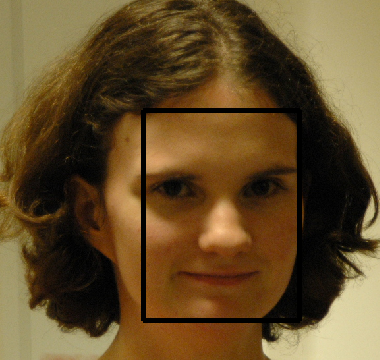
\includegraphics[height=\tempheight]{figures_pami/promo/case1/detector.png}&
\hspace{3mm}
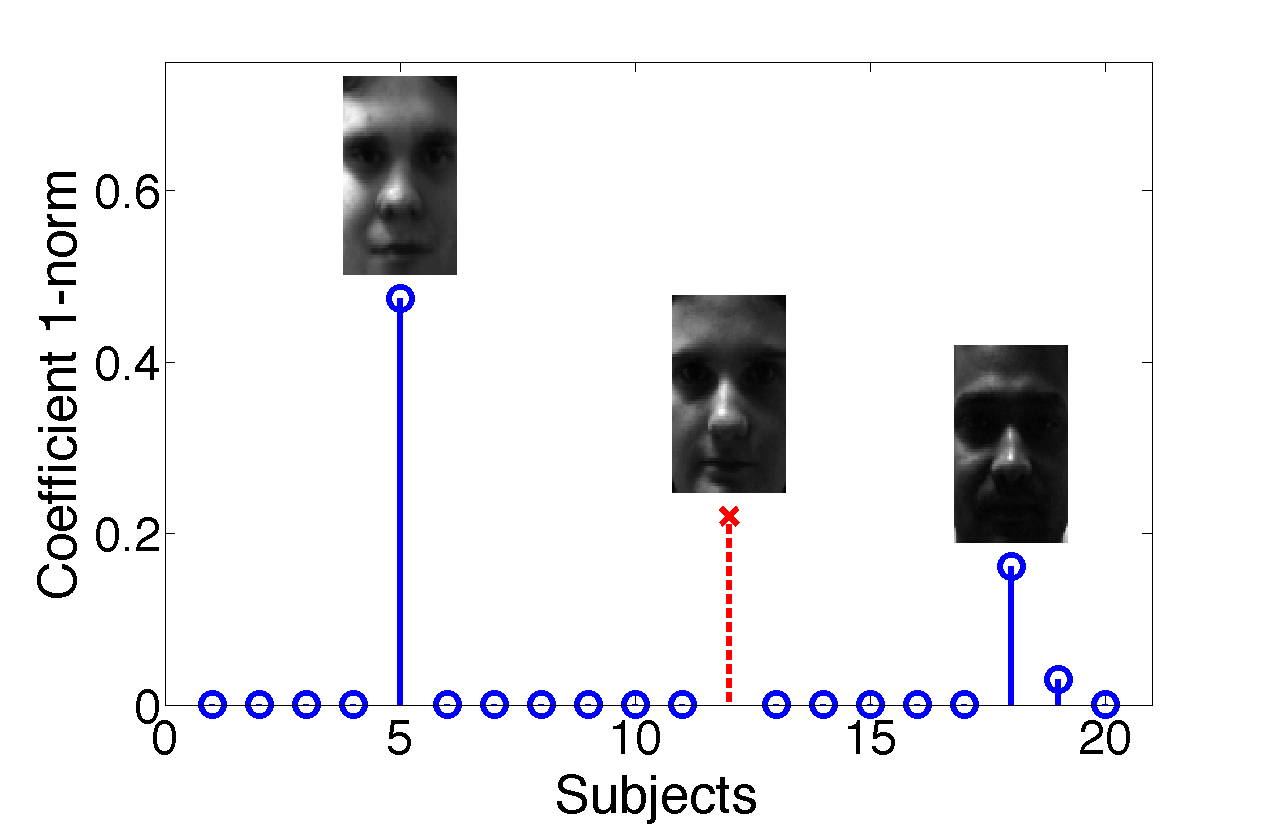
\includegraphics[height=\tempheight]{figures_pami/promo/case1/sci_with_axis_face_case1.png}
\\ 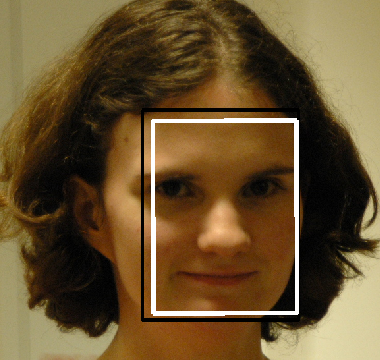
\includegraphics[height=\tempheight]{figures_pami/promo/alignment_and_detector.png}&
\hspace{3mm}
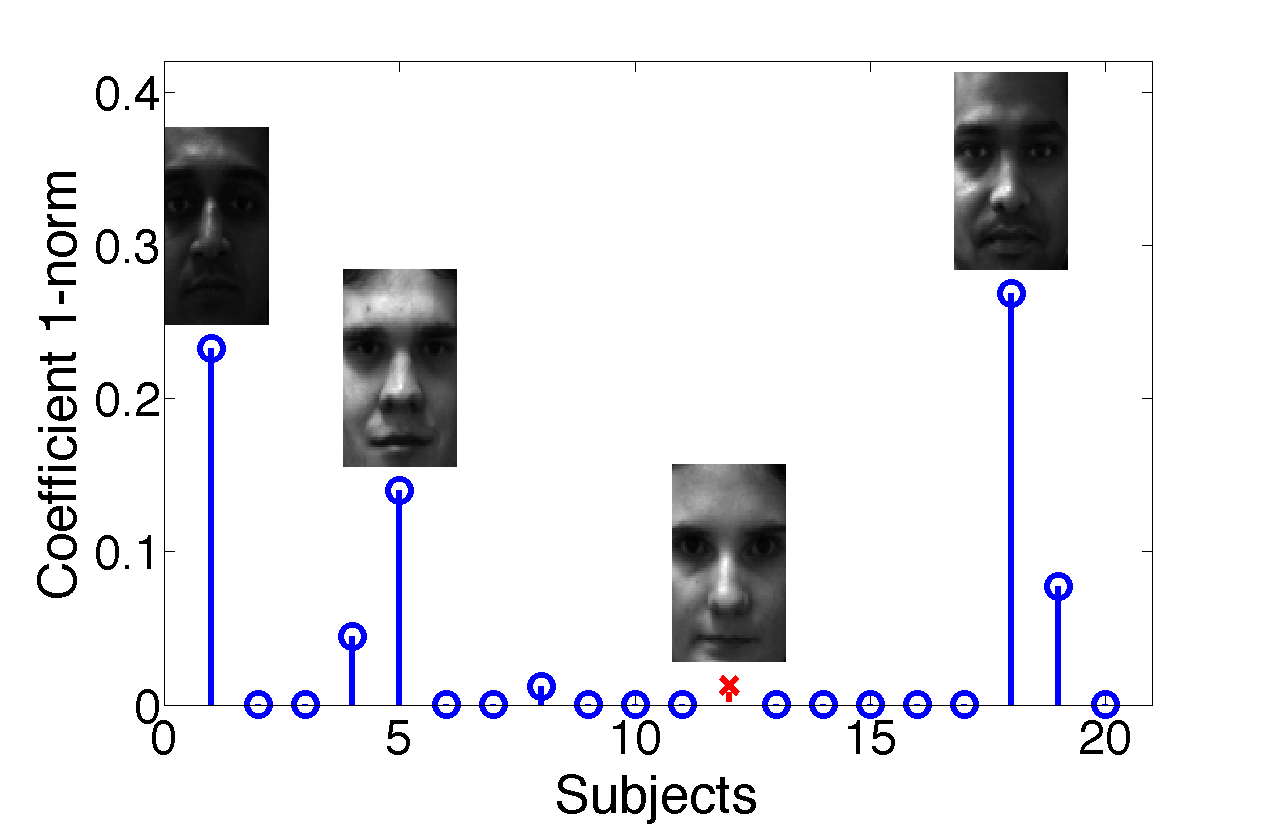
\includegraphics[height=\tempheight]{figures_pami/promo/case2/sci_with_axis_face_case2.png}
\\ 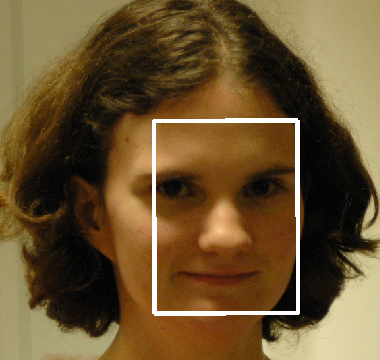
\includegraphics[height=\tempheight]{figures_pami/promo/case3/alignment.png} &
\hspace{3mm}
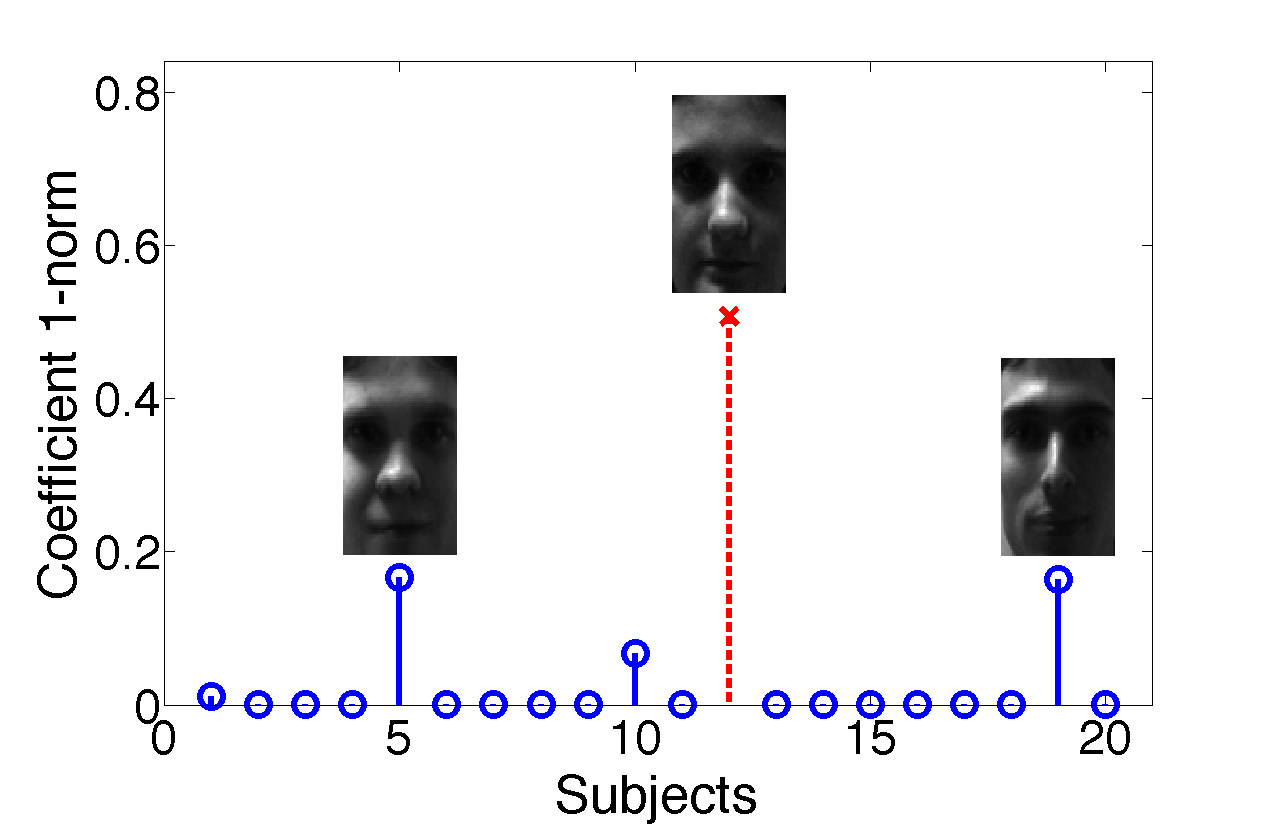
\includegraphics[height=\tempheight]{figures_pami/promo/case3/sci_with_axis_face_case3.png}
\end{tabular} \caption{\small{\bf Effects of registration and illumination on
Recognition}. In this example we identify the girl among 20 subjects, by
computing the sparse representation of her input face with respect to the
entire training set. The absolute sum of the coefficients associated with each
subject is plotted on the right. The weighted sum of the 
subject's training images using the associated sparse coefficients is also shown.
The red line (cross) corresponds to her true identity, subject 12. {\bf Top:} The
input face is from Viola and Jones' face detector (the black box) and all 38
illuminations specified in Section \ref{sec:illumination} are used in the
training.  {\bf Middle:} The input face is well-aligned (the white box) with
the training by our algorithm specified in Section \ref{sec:registration} but
only 24 frontal illuminations are used in the training for recognition (see
Section \ref{sec:illumination}). {\bf Bottom:} The input face is well aligned and
a sufficient set (all 38) of
illuminations are used in the training. Both are necessary for correct recognition
using SRC.}\label{fig:promo}
\end{figure}

\subsection{Relation to Earlier Work on Image Registration}

In holistic recognition algorithms (algorithms that use images themselves as
features) correspondence between points in the test image and in the gallery
images must be achieved.  A long line of research exists on using Active
Appearance Models \cite{Cootes2001-PAMI}, and the closely related Active Shape
Models \cite{cootes1992active} to register images against a relatively
high-dimensional model of plausible face appearances, often leveraging
face-specific contours.  While these model-based techniques have advantages in
dealing with variations in expression and pose, they may add unnecessary
complexity to applications where subjects normally present a neutral face or
only have moderate expression. Instead, this work focuses on classes of
deformations with far fewer degrees of freedom, i.e. similarity transformations
or perspective transformations.  Iterative registration in this spirit of this
work dates at least back to the Lucas-Kanade algorithm
\cite{lucas1981iterative}.

Whereas much of the early work on image registration is aimed at the problem of
registering nearly identical images, say by minimizing a sum of squared
distances or maximizing normalized correlation, face recognition applications
must confront several physical factors simultaneously: misalignment,
illumination variations, and corrupted pixels.  As will be discussed further
below, illumination variation can be dealt with by expressing the test image as
a linear combination of an appropriate set of training images. Similar
representations have been exploited in illumination-robust tracking (e.g.,
\cite{Belhumeur1999-PAA,Murase1995-IJCV}).  For robustness to gross errors, the
$\ell^1$-norm of the residual is a more appropriate objective function than the
classical $\ell^2$-norm. Its use here is loosely motivated by theoretical
results due to Cand\`{e}s and Tao \cite{CandesE2005-IT} (see also
\cite{Wright2008-IT}). These two observations motivate the reformulation of the
registration problem as the search for a set of transformations and
illumination coefficients that minimize the $\ell^1$-norm of the representation
error.  The proposed alignment system uses a generalized Gauss-Newton method
which solves a sequence of affine-constrained $\ell^1$-norm minimization
problems \cite{Osborne1990-JAMSSB,Jittorntrum1980-NM}. Each of these problems
can also be solved efficiently using recently developed first-order techniques
for $\ell^1$-minimization, which are reviewed in \cite{YangA2010-pp}.

% Illumination
Researchers have tried various techniques to deal with illumination variation.
In almost all recognition algorithms where only a single gallery image is
available per individual, illumination effects are regarded as a nuisance that
must be removed before the algorithm can continue.  This is typically done by
making statistical assumptions about how illumination affects the image, and
using those assumptions to extract a new representation that is claimed to be
illumination invariant.  Recent examples include \cite{chen2006total} and
\cite{zhou2007appearance}.  Despite these efforts, truly
illumination-invariant features remain difficult to obtain from a single input
image.  Clearly, if one has the luxury of designing the acquisition system
and the application demands a high recognition rate,
it is then unwise to limit the gallery to a
single image per person.  The proposed recognition system therefore takes the strategy of sampling many
gallery images of each individual under varying illuminations.  These images
are used as the basis for either a convex cone model
\cite{Georghiades2001-PAMI,belhumeur1998set}, or a subspace model
\cite{Basri2003-PAMI}.  Images are captured using a simple-to-construct
projector based light stage.  While similar systems have been used for
other applications, to our knowledge, this
system is the first to use projectors to indirectly illuminate a subject's face for
the purpose of face recognition.

\subsection{Contributions} This chapter demonstrates how registration and
illumination can be simultaneously addressed within a robust sparse
representation framework. Face registration, despite being a challenging
nonlinear problem, can be solved by a series of linear programs that
iteratively minimize the sparsity of the registration error. This leads to an
efficient and effective alignment algorithm for face images that works for a
large range of variation in translation, rotation, and scale, even when the
face is only partially visible due to eyeglasses, closed eyes and open mouth,
sensor saturation, etc.  A sufficient set of training illuminations that is
capable of linearly representing typical indoor and outdoor lighting is
determined empirically, and a practical hardware system based on synchronized
cameras and projectors is developed for capturing them.

%A key part of the system is exploiting
%an important property of the imaging process:  there is a linear mapping
%between the space of illuminations of an object, and the space of images of
%that object taken under the same pose.  This makes it possible to effectively
%model the testing image as a linear superposition of a large (and well chosen)
%set of training images.  This idea is certainly not new; indeed it has been in
%use for face recognition for roughly two decades, \cite{Turk1991-CVPR}.
%However, traditional algorithms that rely on this property of the image
%formation process have tended to perform very badly in the face of occlusions
%and when highly quality training images are unavailable.  

The chapter then demonstrates the effectiveness of the proposed new
methods with a complete face recognition system that is {\em
simple, stable, and scalable}. The proposed system performs
robust automatic recognition of subjects from loosely
controlled probe images taken both indoors and outdoors,
using a gallery of
frontal views of the subjects' faces under the proposed
illuminations. An off-the-shelf face
detector\footnote{We use the OpenCV
implementation of the Viola and Jones' face detector
\cite{Viola2004-IJCV}.} is used to detect faces in the test images.

Extensive experiments are conducted on the proposed system with
both public databases and a face database that is collected by
the proposed acquisition system. The experimental results on
large-scale public face databases show that the algorithm
indeed achieves very good performance on these databases,
exceeding or competing with the state-of-the-art algorithms.
Additionally, the experimental results on the private database
clearly demonstrate that the recognition system not only works well with
images taken under controlled laboratory conditions, but is
capable of handling practical indoor and outdoor illuminations as well.

\noindent{\em Organization of this chapter:} Section \ref{sec:registration},
presents a derivation of the robust registration and recognition algorithm within the sparse
representation framework. It further elaborates on algorithmic implementation issues,
conducts region of attraction experiments with respect to both 2D in-plane
deformation and 3D pose variation, and discusses its relationship to existing
work. Section \ref{sec:illumination} is dedicated to the training acquisition
system. This system is used to investigate empirically how many training
illuminations are required to handle practical illumination variations, and to
suggest a sufficient set of 38 training illuminations. Extensive experiments on
a large-scale public database and on a newly gathered database are conducted in Section
\ref{sec:multipie} and Section \ref{sec:own-data}, respectively, to verify the
proposed system. 

\section{Robust Alignment}\label{sec:registration} As demonstrated in Figure
\ref{fig:promo}(top), the main limitation of the {\em Sparse Representation and
Classification} (SRC) algorithm of \cite{Wright2009-PAMI} is the assumption of
pixel-accurate alignment between the test image and the training set. This
leads to brittleness under pose and misalignment, making it inappropriate for
deployment outside a laboratory setting. The goal of this section is to show
how this weakness can be rectified while still preserving the conceptual
simplicity and good recognition performance of SRC.

SRC assumes access to a database of multiple registered
training images per subject, taken under varying illuminations.
The images of subject $i$, stacked as vectors, form a matrix
$A_i \in \Re^{m \times n_i}$. Taken together, all of the images
form a large matrix $A = [ A_1 \mid A_2 \mid \dots \mid A_K ]
\in \Re^{m \times n}$. As argued in \cite{Wright2009-PAMI}, a
well-aligned test image $\y_0$ can be represented as a sparse
linear combination $A \x_0$ of all of the images in the
database,\footnote{This assumes that the training illuminations are sufficient. The next section will address how to ensure illumination
sufficiency.} plus a sparse error $\e_0$
due to corrupted pixels. The sparse representation can be recovered by
minimizing the $\ell^1$-norm\footnote{The $\ell^1$-norm of a
vector, denoted by $\|\cdot\|_1$, is the sum of absolute values of its entries.} of
$\x$ and $\e$:
\begin{equation}
\min_{\x,\e} \, \| \x \|_1 + \| \e\|_1 \quad \subj \quad \y_0 = A \x + \e.
\label{eqn:robust-l1}
\end{equation}
Now suppose that $\y_0$ is subject to some pose or
misalignment, so that instead of recording $\y_0$, the camera captures
a warped image $\y = \y_0 \circ \tau^{-1}$, for some
transformation $\tau \in T$ where $T$ is a finite-dimensional
group of transformations acting on the image domain.  The
transformed image $\y$ no longer has a sparse representation of
the form $\y = A \x_0 + \e_0$, and naively applying the
algorithm of \cite{Wright2009-PAMI} is no longer appropriate,
as seen in Figure \ref{fig:promo}(top).

\subsection{Batch and Individual Alignment} If the
true deformation $\tau^{-1}$ can be found, then
its inverse $\tau$ can be applied to the test image and it again becomes
possible to find a sparse representation of the resulting
image, as $\y \circ \tau = A \x_0 + \e_0$.\footnote{In the terminology of \cite{baker2004lucas}, this formulation is ``Forward Additive''.}
  This sparsity
provides a strong cue for finding the correct deformation
$\tau$: conceptually, one would like to seek a transformation
$\tau$ that allows the sparsest representation, via
\begin{equation} \label{eqn:L1-L1-conceptual}
\hat{\tau} = \arg\hspace{-2.5mm}\min_{\x,\e,\tau \in T} \| \x \|_1 + \| \e \|_1 \quad \subj \quad \y \circ \tau = A \x + \e.
\end{equation}
For fixed $\tau$, this problem is jointly convex in $\x$ and
$\e$. However, as a simultaneous optimization over the
coefficients $\x$, error representation $\e$, and
transformation $\tau$, it is a difficult, non-convex
optimization problem. One source of difficulty is the presence
of multiple faces in the matrix $A$:
\eqref{eqn:L1-L1-conceptual} has many local minima that
correspond to aligning $\y$ to different subjects. In this
sense, the misaligned recognition problem differs from the
well-aligned version studied in \cite{Wright2009-PAMI}. For the
well-aligned case, it is possible to directly solve for a
global representation, with no concern for local minima. With
possible misalignment, it is more appropriate to seek the best
alignment of the test face with each subject $i$:
\begin{equation} \label{eqn:per-subject-L1}
\hat \tau_i = \arg\hspace{-2.5mm}\min_{\x,\e,\tau_i \in T} \| \e \|_1 \quad \subj \quad \y \circ \tau_i = A_i \x + \e.
\end{equation}
It no makes sense to penalize $\| \x \|_1$, since $A_i$ consists of
only images of subject $i$ and therefore $\x$ is no longer expected to
be sparse.

\subsection{Alignment via Sequential $\ell^1$-Minimization} While the problem
\eqref{eqn:per-subject-L1} is still non-convex, for cases of practical interest
in face recognition, a good initial guess for the transformation is available,
e.g., from the output of a face detector. This initialization can be refined to
approach an estimate of the true transformation by repeatedly linearizing about  the
current estimate of $\tau$, and seeking representations of the form:
\begin{equation}
\y\circ \tau + J \Delta \tau = A_i \x + \e.
\end{equation}
Here, $J = \frac{\partial}{\partial \tau} \y \circ \tau$ is the Jacobian of $\y
\circ \tau$ with respect to the transformation parameters $\tau$, and $\Delta
\tau$ is the step in $\tau$. The above equation is under-determined if the
registration error $\e$ is allowed to be arbitrary. At the correct alignment it
is expected that the test image only differs from $A_i \x$ only for the
minority of the pixels corrupted by occlusions. Thus, the algorithm computes a
deformation step $\Delta \tau$ that best sparsifies the registration error
$\e$, in terms of its $\ell^1$-norm:
\begin{equation}
\Delta\hat{\tau}_1 = \arg\hspace{-3.5mm}\min_{\x,\e,\Delta\tau \in T} \| \e \|_1 \quad \subj \quad \y\circ\tau + J \Delta \tau = A_i \x + \e.
\label{eqn:L1-align}
\end{equation}
This is different from the popular choice that
minimizes the $\ell^2$-norm of the registration error:
\begin{equation}
\Delta\hat{\tau}_2 = \arg\hspace{-3.5mm}\min_{\x,\e,\Delta\tau \in T} \| \e \|_2 \quad \subj \quad \y\circ\tau + J \Delta \tau = A_i \x + \e,
\label{eqn:L2-align}
\end{equation}
which is also equivalent to finding the deformation step
$\Delta  \tau$ by solving the least-square problem:
$\min_{\x,\Delta \tau} \|\y \circ \tau + J\Delta \tau - A_i \x
\|_2$. Empirically, if there is only small noise
between $\y_0$ and $A_i\x$, both \eqref{eqn:L1-align} and
$\eqref{eqn:L2-align}$ have similar performance.  However, if
there are occlusions in $\y_0$, sequential
$\ell^1$-minimization \eqref{eqn:L1-align} is significantly
better than sequential $\ell^2$-minimization
\eqref{eqn:L2-align}. Figure \ref{fig:L1-L2-align} shows an
example.

The scheme \eqref{eqn:L1-align} can be viewed as a generalized Gauss-Newton
method for minimizing the composition of a non-smooth objective function (the
$\ell^1$-norm) with a differentiable mapping from transformation parameters to
transformed images. Such algorithms date at least back to the 1970's
\cite{Cromme1978-NM,Jittorntrum1980-NM}, and continue to attract attention
today \cite{Lewis2008-TR}. While a detailed discussion of their properties is
outside the scope of this thesis, it is worth mentioning that the scheme
\eqref{eqn:L1-align} is known to converge quadratically in the neighborhood of
any local optimum of the $\ell^1$-norm. In practice, this means that $\approx$
10 to 15 iterations suffice to reach the desired solution. The
interested reader is referred to \cite{Jittorntrum1980-NM,Osborne1990-JAMSSB} and the
references therein.

\renewcommand{\tempheight}[0]{1.0in}
\begin{figure}
\centering
{
\begin{tabular}{cccc}
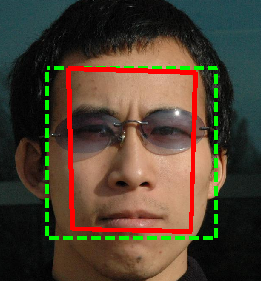
\includegraphics[height=\tempheight]{figures_pami/L1_cropped} &
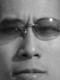
\includegraphics[height=\tempheight]{figures_pami/y_warp_L1} &
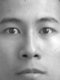
\includegraphics[height=\tempheight]{figures_pami/y_hat_L1} &

\includegraphics[height=\tempheight]{figures_pami/e_L1} \\
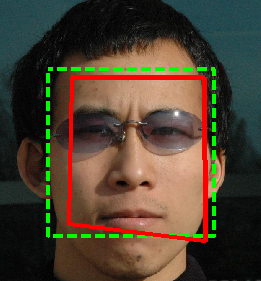
\includegraphics[height=\tempheight]{figures_pami/L2_cropped} &
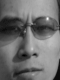
\includegraphics[height=\tempheight]{figures_pami/y_warp_L2} &
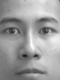
\includegraphics[height=\tempheight]{figures_pami/y_hat_L2} &
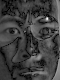
\includegraphics[height=\tempheight]{figures_pami/e_L2} \\
(a) & (b) & (c) & (d)
\end{tabular}}
\caption{\small{\bf Comparing alignment of a subject wearing sunglasses by
$\ell^1$ and $\ell^2$ minimization.}
{\bf Top:} alignment result of minimizing $\|\e\|_1$; {\bf Bottom:}
result of minimizing $\|\e\|_2$. (a) {\em Green (dotted):} Initial face boundary
given by the face detector, {\em Red (solid):} Alignment result shown on the same
face; (b) warped testing image using the estimated transformation $\y_0$;
(c) reconstructed face $A_i\x$ using the training; (d) image of error $\e$. }\label{fig:L1-L2-align}
\end{figure}

In addition to normalizing the training images (which is done
once), it is important to normalize the warped testing image
$\y \circ \tau$ as the algorithm runs.  Without normalization,
the algorithm may fall into a degenerate global minimum
corresponding to zooming in on a dark region of the test
image.  Normalization is done by replacing the linearization of
$\y \circ \tau$ with a linearization of the normalized version
$\tilde \y(\tau) = \frac{\y \circ \tau}{\|\y \circ \tau\|_2}$.
The proposed alignment algorithm can be easily extended to work
in a {\em multiscale} fashion, with benefits both in
convergence behavior and computational cost.  The alignment
algorithm is simply run to completion on progressively less
downsampled versions of the training and testing images, using
the result of one level to initialize the next.

\subsection{Robust Recognition by Sparse Representation} Once
the best transformation $\tau_i$ has been computed for each
subject $i$, the training sets $A_i$ can be aligned to $\y$,
and a global sparse representation problem of the form
\eqref{eqn:robust-l1} can be solved to obtain a discriminative
representation in terms of the entire training set. Moreover,
the per-subject alignment residuals $\| \e \|_1$ can be used to
prune unpromising candidates from the global optimization,
leaving a much smaller and more efficiently solvable problem.
The complete optimization procedure is summarized as Algorithm
\ref{alg:deformable-src}. The parameter $S$ is the number of subjects
considered together to provide a sparse representation for the
test image. If $S = 1$, the algorithm reduces to classification
by registration error; but considering the test image might be
an invalid subject, $S=10$ is typically chosen. Since valid
images have a sparse representation in terms of this larger
set, invalid test images can be rejected using the {\em sparsity
concentration index} proposed in \cite{Wright2009-PAMI}.
The function $\delta_i(\x)$ in Algorithm \ref{alg:deformable-src}
selects coefficients from the vector $\x$ corresponding to subject $i$.

Another important free parameter in Algorithm \ref{alg:deformable-src} is the
class of deformations $T$. In the experiments presented here, 2D similarity
(i.e. 2D rigid transformations) transformations are used, $T =
\mathbb{SE}(2)\times \Re_+$\footnote{Here, SE stands for Special Euclidean.
The $\Re_+$ accounts for the scale.}, for removing alignment error incurred by
face detector, or 2D projective transformations, $T =
\mathbb{GL}(3)\footnote{Here, GL stands for General Linear.  This class of
transformations is able to represent distortion in a perspective image of a
planar object.}$, for handling some pose variation.

Algorithm \ref{alg:deformable-src}, also implements a simple heuristic
motivated by the observation that the face detector output may be poorly
centered on the face and may contain a significant amount of the background:
before the recognition stage, instead of aligning the training sets to the
original $\y$ directly obtained from the face detector, the transformations of
the top $S$ classes $\tau_{k_1}, \tau_{k_2}, \ldots, \tau_{k_S}$ are averaged
into a transformation $\bar{\tau}$.  Updating $\y$ according to $\bar{\tau}$
results in a better centered test image. For the 2D similarity transformations,
which are used in our system when initialized by the face detector, a
transformation $\tau$ can be parameterized as $\tau = (\tau^1, \tau^2, \tau^3,
\tau^4)$, where $\tau^1$ and $\tau^2$ represent the translations in $x$- and
$y$-axis, $\tau^3$ represents the rotation angle and $\tau^4$ represents the
scale. The average transformation is simply obtained by taking the
component-wise mean:
\begin{displaymath}
\bar{\tau}^i = (\tau_{k_1}^i + \tau_{k_2}^i + \cdots +
\tau_{k_S}^i) / S, i = 1,2,3,4.
\end{displaymath}
Finally, the training sets are aligned to the new $\y$.

\begin{algorithm}[thb]
\caption{\bf\small (Deformable Sparse Recovery and Classification for
Face Recognition)} \label{alg:deformable-src}
\begin{algorithmic}[1]
\begin{small}
\STATE {\bf Input:} Training images $\{A_i \in \Re^{m\times n_i}\}_{i=1}^K$ for $K$ subjects,  a test image
$\bb\in\Re^m$ and a deformation group $T$.
\STATE
{\bf for} each subject $i$,
\STATE \hspace{3mm} $\tau^{(0)}
\leftarrow I$.
\STATE \hspace{3mm} {\bf while} not converged $(j=1,2,\ldots)$ {\bf do}
\STATE \hspace{6mm}
$\tilde \bb(\tau) \leftarrow \frac{\bb \circ \tau}{\|\bb \circ
\tau\|_2}$; \;\;\; $J \leftarrow  \frac{\partial}{\partial
\tau} \tilde\bb(\tau)  \bigr|_{\tau^{(j)}} $;
%\STATE \hspace{6mm} $(\hat \x, \hat \e, \Delta \tau) \leftarrow \left\{\begin{array}{l} \arg \min_{\x,\e,\Delta \tau} \| \e \|_1 \\  \subj \; \bb + J \Delta \tau = A_k \x + \e \end{array}\right.$
\STATE \hspace{6mm} $ \Delta \tau =  \arg\min \; \| \e \|_1  \;
\subj \; \tilde \bb + J \Delta \tau = A_i \x + \e.$
\STATE
\hspace{6mm} $\tau^{(j+1)} \leftarrow \tau^{(j)} + \Delta
\tau$;
\STATE \hspace{3mm} {\bf end while} \STATE {\bf end} \STATE Keep
the top $S$ candidates $k_1, \ldots, k_S$ with the smallest
residuals $\|\e\|_1$. \STATE Compute an average transformation
$\bar{\tau}$ from $\tau_{k_1}, \tau_{k_2}, \ldots, \tau_{k_S}$.
\STATE Update $\bb \leftarrow \bb \circ \bar{\tau}$ and $\tau_i
\leftarrow \tau_i \cdot \bar{\tau}^{-1}$ for $i = k_1, \dots,
k_S$. \STATE Set $A \leftarrow \big[ A_{k_1} \circ
\tau_{k_1}^{-1} \mid A_{k_2} \circ \tau_{k_2}^{-1} \mid \dots
\mid A_{k_S} \circ \tau_{k_S}^{-1} \big]$. \STATE Solve the
$\ell_1$-minimization problem: \\
\hspace{2em}$\hat{\x} = \arg \min_{\x, \e} \| \x \|_1 + \|\e\|_1 \;\; \subj \;\; \bb = A \x + \e.$
\STATE Compute residuals $r_i(\bb) = \| {\bb} - {A}_i \, \delta_i(\hat{\x}) \|_2$ for $i = k_1, \dots, k_S$.
\STATE {\bf Output:} $\mbox{identity}(\bb) = \arg\min_i r_i(\bb)$.
\end{small}
\end{algorithmic}
\end{algorithm}
%\vspace{-4mm}


The transformation $\tau$ defines a mapping between the coordinates of pixels
in the large original image and a smaller (un)warped image. The pixels of the
small image are stacked into a vector. To prevent aliasing artifacts in the
downsampled image, it is necessary to apply a smoothing filter to the original
image beforehand. For a simple implementation, a rectangular window with
regular sampling can used, but in general, the small image need not be
regularly sampled in pixel coordinates.  For example, the sample locations
could be arbitrarily selected from within a ``face shaped'' area. The impact of
non-rectangular sampling windows on performance of the algorithm will be
discussed in Section \ref{sec:multipie}.

\subsection{System Implementation}
The runtime of Algorithm~\ref{alg:deformable-src} is dominated
by the time spent solving two qualitatively similar $\ell_1$ minimization problems.
Custom $\ell_1$ minimization solvers for this purpose based on
\emph{Augmented Lagrange Multiplier} (ALM) algorithm have been developed.
the ALM algorithm was selected because it strikes the best
balance between speed, accuracy, and scalability.  Several $\ell_1$ minimization
algorithms were tested for the face recognition problem, 
and ALM was found to have the best performance. 
A more in-depth discussion of the solvers will be presented
in Chapter \ref{chap:minimization}
For a more detailed discussion of competing
approaches, the interested reader is referred to
\cite{YangA2010-pp}.
On a Mac Pro with
two Dual-Core 2.66GHz Xeon processors and 4GB memory,
running on a private database containing images size $80\times 60$
pixels from 109 subjects under 38 illuminations,
the C++ implementation of Algorithm~\ref{alg:deformable-src} takes
about 0.60 seconds per subject for alignment and about 2.0
seconds for global recognition. Compared to the highly
customized interior point method first presented in 
\cite{Wagner2009-CVPR}, this new algorithm is
only slightly faster for per subject alignment. However, it is
much simpler to implement and it achieves a
\emph{speedup of more than a factor of 10} for global
recognition!  Performance optimization of this algorithm
will be discussed in Chapter \ref{chap:parallel}.

\subsection{Experiments on Region of Attraction} Three experimental results
will now be presented to demonstrate the effectiveness of the individual
alignment procedure outlined in the previous section. They show sufficiency of
the region of attraction, verify effectiveness of the multiscale extension, and
show stability to small pose variations.  After a discussion of illumination
invariance in the next section, large-scale recognition experiments are
presented in Sections \ref{sec:multipie} and \ref{sec:own-data}.

\noindent {1) \em 2D Deformation.}  The first experiment verifies the
    effectiveness of our alignment algorithm with images
    from the CMU Multi-PIE Database \cite{Gross2008-FGR}.
    The gallery set consists of all the subjects in Session 1, using 7
    illuminations per person. The test images use
    one new illumination from each user in Session
    2.\footnote{The training are illuminations $\{0, 1, 7,
    13, 14, 16, 18\}$ of \cite{Gross2008-FGR}, and the
    testing is the illumination 10. } A ground truth for
	registration is formed by manually selecting
    eye corners in both training and testing images. 
	The images are downsampled to a canonical image size of 
    $80\times 60$ pixels\footnote{Unless otherwise stated,
    this will be the default resolution at which 
    all training and testing datasets are resampled.} 
	and the distance between the two outer
    eye corners is normalized to be 50 pixels for each
    person. An artificial deformation is applied to the
    testing image with a combination of translation,
    rotation and scaling. A small value for the alignment
    error $r = \|\e\|_1$ is chosen as an indicator of success. Let $r_0$
    be the alignment error obtained by aligning a test
    image to the training images without any artificial
    perturbation. After the test image is artificially
    perturbed and aligned resulting in an alignment error
    $r$, we consider the alignment successful if $|r - r_0 | \leq
    0.01r_0$. Figure \ref{fig:attraction} shows the
    percentage of successful registrations for all subjects
    for each artificial deformation. The results suggest
    that the alignment algorithm works extremely well with
    translation up to 20\% of the eye distance (or 10
    pixels) in all directions and up to $30^\circ$ in-plane
    rotation. Tests of the alignment algorithm
    with scale variation show that it can handle up to 15\%
    change in scale.

In order to determine if this region of attraction is sufficient,
it must be compared to the accuracy achieved by the initialization
provided by the face detector.  Statistics of the Viola and Jones'
 face detector on the Multi-PIE dataset. For 4,600 frontal
 images of 230 subjects under 20 different illuminations,
 using manual registration as the ground truth, the average
 misalignment error of the detected faces is about 6 pixels
 and the average variation in scale is 8\%. This falls
 safely inside the region of attraction for our alignment
 algorithm.
\newcommand{\tempheighta}[0]{1.1in}
\newcommand{\tempheightb}[0]{0.9in}
\begin{figure*}
\centering
{
\begin{tabular}{ccc}
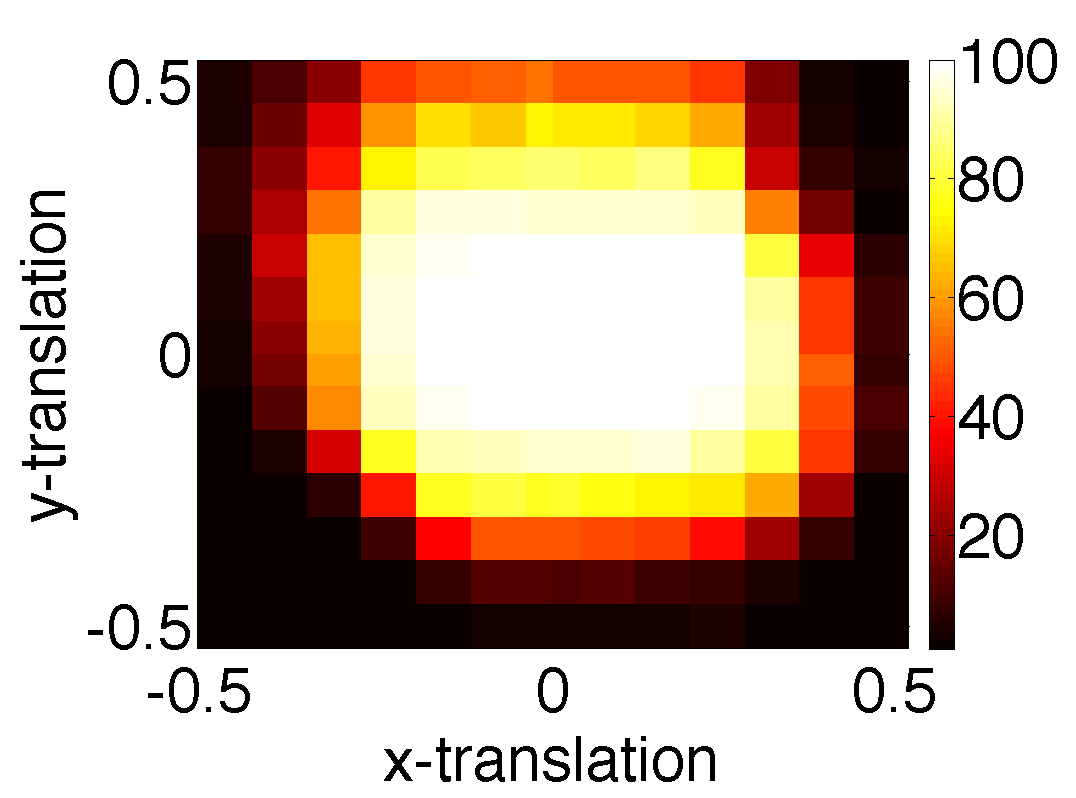
\includegraphics[height=\tempheighta]{figures_pami/x_y_roa.png} &
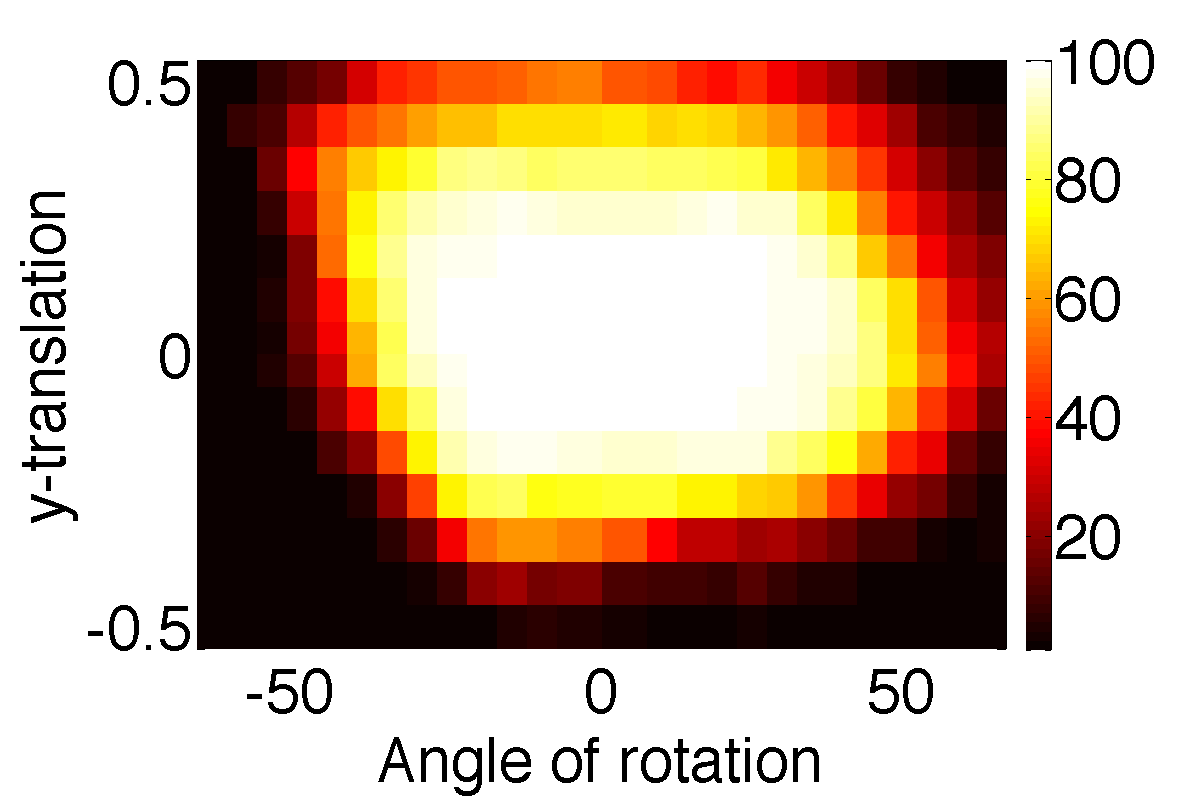
\includegraphics[height=\tempheighta]{figures_pami/y_theta_roa.png} &
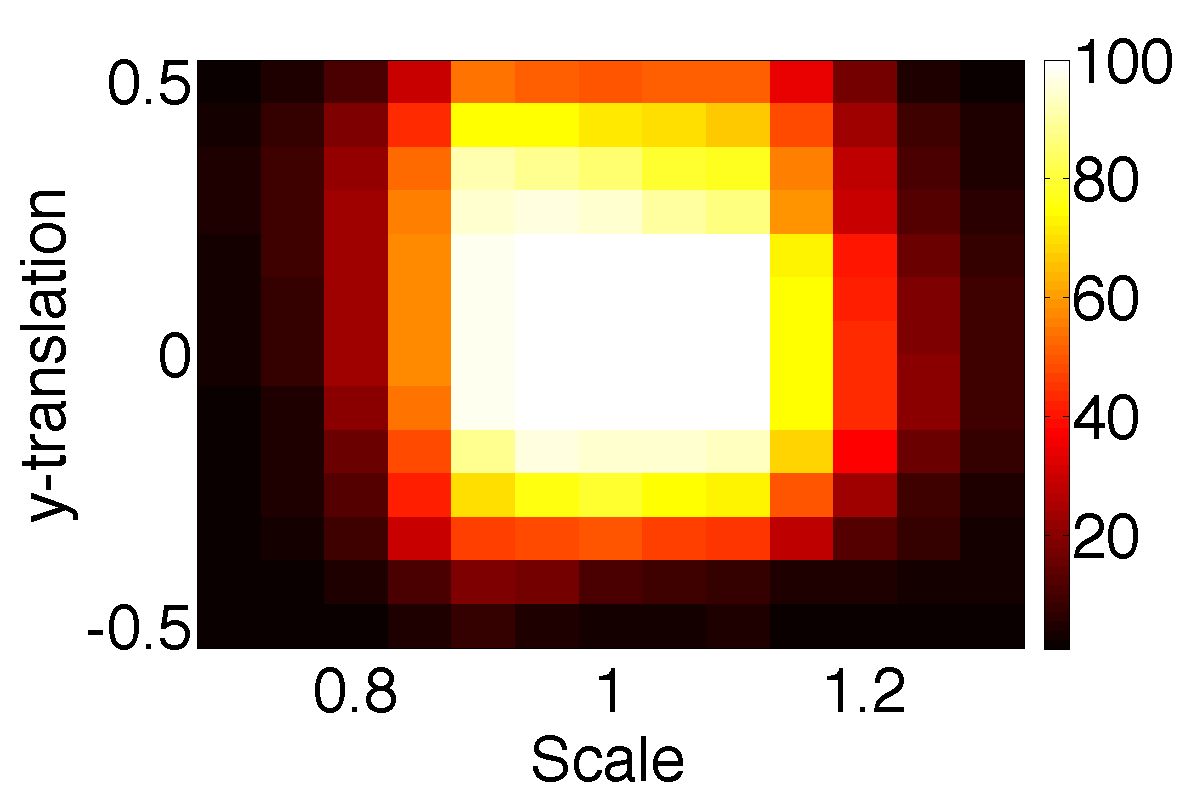
\includegraphics[height=\tempheighta]{figures_pami/y_s_roa.png}\\
(a)&(b)&(c)
\end{tabular}
\begin{tabular}{cccc}
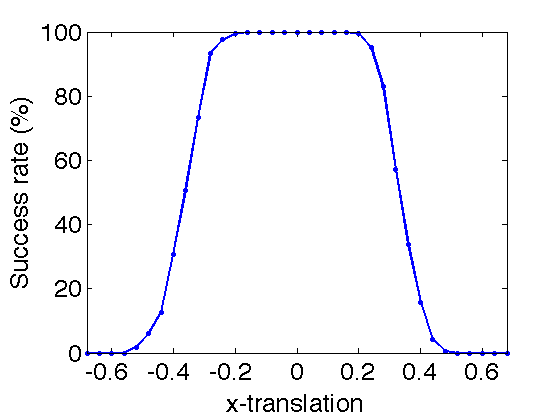
\includegraphics[height=\tempheightb]{figures_pami/x_tr.png} &
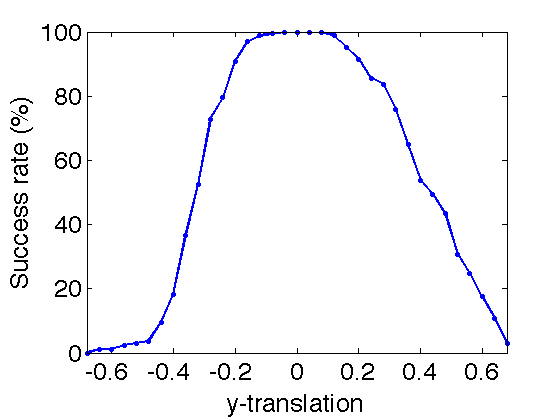
\includegraphics[height=\tempheightb]{figures_pami/y_tr.png} &
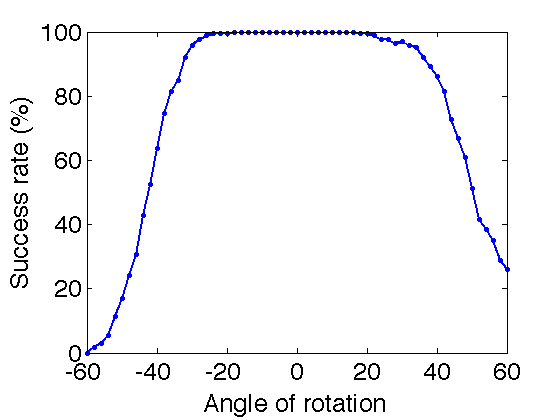
\includegraphics[height=\tempheightb]{figures_pami/theta.png} &
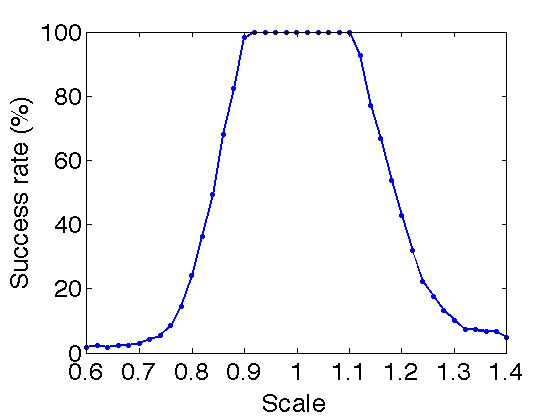
\includegraphics[height=\tempheightb]{figures_pami/scale.png}\\
(d)&(e)&(f)& (g)
\end{tabular}
} \caption{\small{\bf Region of attraction.} Fraction of
subjects for which the algorithm successfully aligns a
synthetically perturbed test image.  The amount of translation
is expressed as a fraction of the distance between the outer
eye corners, and the amount of in-plane rotation in degrees.
{\bf Top row:} (a) Simultaneous translation in $x$ and $y$
directions. (b) Simultaneous translation in $y$ direction and
in-plane rotation. (c) Simultaneous translation in $y$
direction and scale variation. {\bf Bottom row:} (d)
Translation in $x$ direction only. (e) Translation in $y$
direction only. (f) In-plane rotation only. (g) Scale variation
only.} \label{fig:attraction} 
\end{figure*}

\noindent{2) \em Multiscale Implementation.}
Performing alignment in a multiscale fashion has two benefits: first, it provides a larger region of attraction, and second, it reduces overall computational cost. Here, we further investigate the convergence behavior of the algorithm as a function of the standard deviation $\sigma$ of the Gaussian smoothing filter and the number of scales considered.
We use the same 7 illuminations in
Session 1 as training, and all 20 illuminations in the same
session as testing. We introduce artificial deformation in
both $x$ and $y$ directions up to 16 pixels in the
$80\times 60$ frame, with a step size of 4 pixels, i.e.,
$(\Delta x, \Delta y) \in \{-16,-12,\ldots,12,16\} \times
\{-16,-12,\ldots,12,16\}$. We consider an alignment
successful if the estimated coordinates of the eye-corners
are within 1 pixel from the ground truth in the original
image.  In Figure \ref{fig:multiscale}, we report the
alignment success rate, averaged over the artificially
perturbed initial deformations, as a function of the
standard deviation of the Gaussian kernel $\sigma$, for
three choices of the number of scales. As one can see,
using multiscale indeed improves the performance, and when
3 scales are used, a smaller convolution kernel can achieve
a similar performance compared to a much larger kernel when
only 2 scales are used.
\begin{figure}
\centering
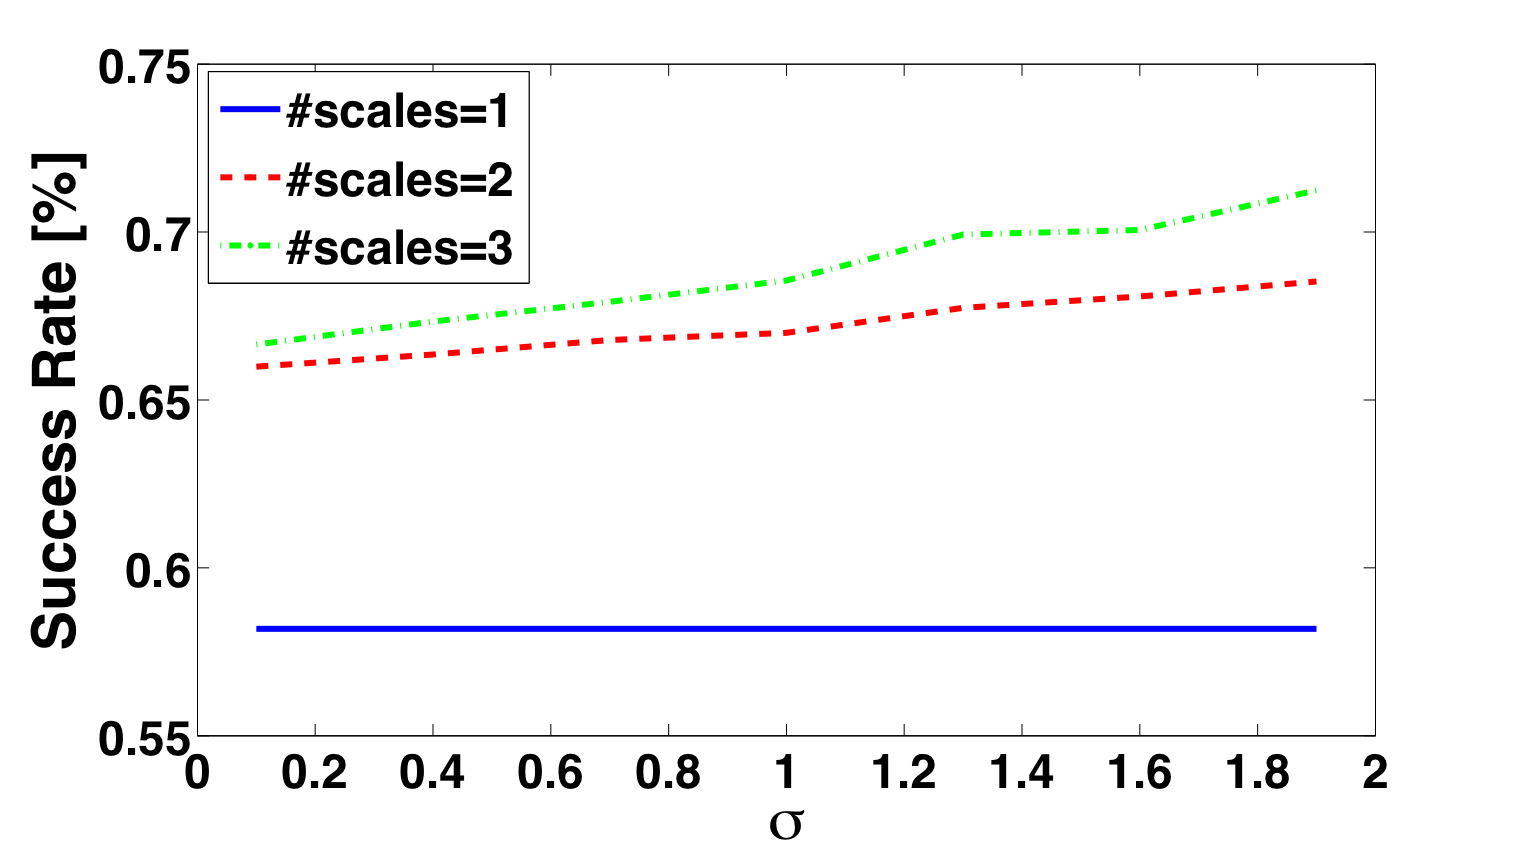
\includegraphics[width=4in]{figures_pami/multiscale.png}
\caption{\small{\bf Multiscale alignment.} This figure shows the average success rate of alignment over all possible perturbations. A smaller blur kernel can be applied to achieve certain level of performance when more scales are used.}
\label{fig:multiscale}
\end{figure}

\noindent{3) \em 3D Pose Variation.} As densely sampled pose
and
    illumination face images are not available in any of
    the public databases, including Multi-PIE, we have
    collected our own dataset using our own system (to be
    introduced in the next section). We use frontal face
    images of a subject under the 38 illuminations proposed
    in the next section as training. For testing, we
    collect images of the subject under a typical indoor
    lighting condition at pose ranging from $-90^\circ$ to
    $+90^\circ$ with step size 5.625$^\circ$, a total of 33
    poses. We use Viola and Jones' face detector to
    initialize our alignment algorithm.
Figure \ref{fig:pose-alignment} shows that our algorithm works reasonably well with poses up
to $\pm 45^\circ$.
Note that this level of out-of-plane
 pose variation is beyond what we intend to handle with our formulation.
\begin{figure}
\centering
{
\begin{tabular}{ccccc}
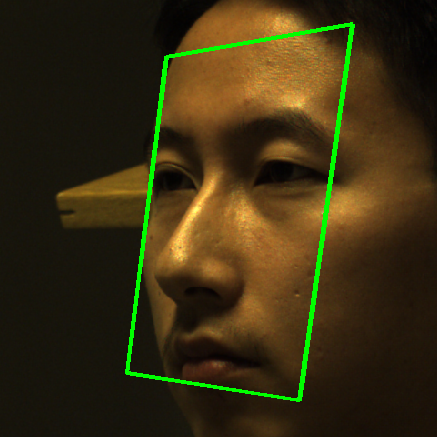
\includegraphics[height=1in]{figures_pami/5} &
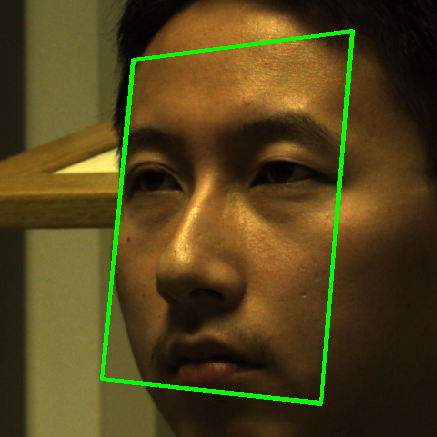
\includegraphics[height=1in]{figures_pami/7} &
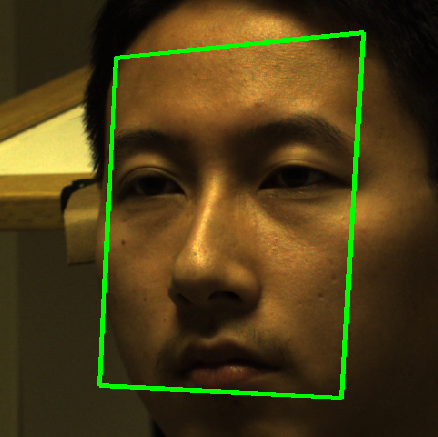
\includegraphics[height=1in]{figures_pami/09} &
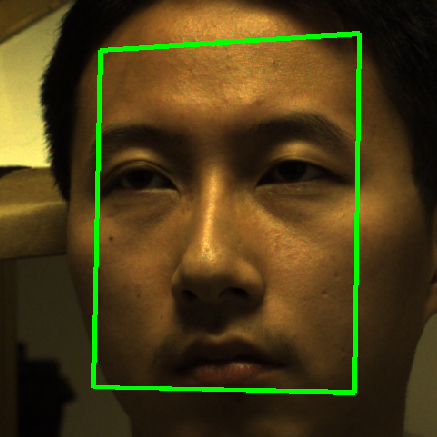
\includegraphics[height=1in]{figures_pami/11} &
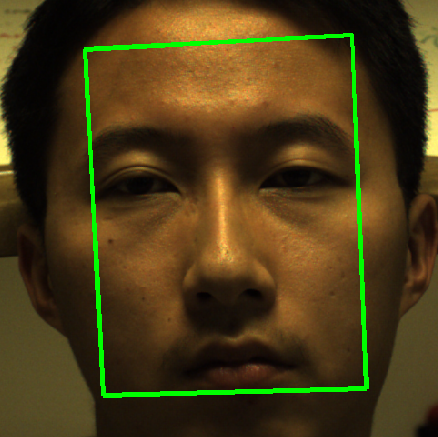
\includegraphics[height=1in]{figures_pami/13} \\
(a) & (b) & (c) & (d) & (e)\\
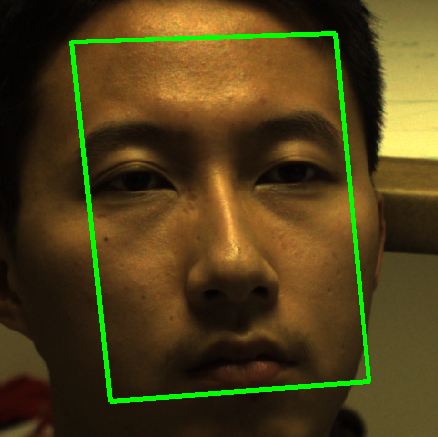
\includegraphics[height=1in]{figures_pami/15} &
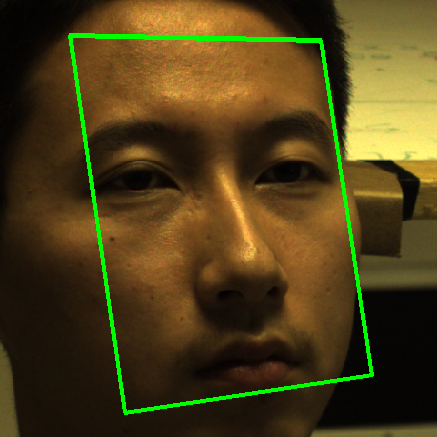
\includegraphics[height=1in]{figures_pami/17} &
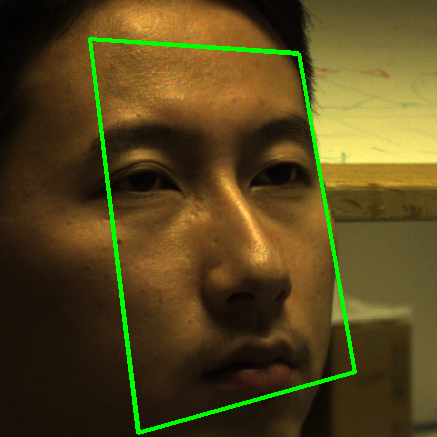
\includegraphics[height=1in]{figures_pami/19} &
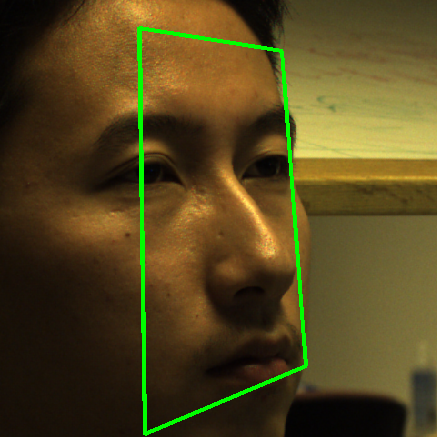
\includegraphics[height=1in]{figures_pami/21} &
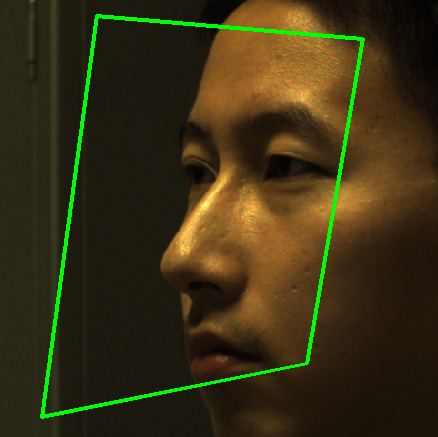
\includegraphics[height=1in]{figures_pami/3} \\
(f) & (g) & (h) & (i) & (j)
\end{tabular}
}
\caption{\small{\bf 2D Alignment of test images with different poses to frontal training images.} {\bf (a) to (i):}  plausible alignment for pose from $-45^{\circ}$
to $+45^{\circ}$. {\bf (j):} a case when the algorithm fails for an extreme pose ($>45^{\circ}$).
}\label{fig:pose-alignment} 
\end{figure}
\subsection{Comparison with Related Work}
Our modification to SRC roots solidly in the tradition of
adding deformation-robustness to face recognition algorithms
\cite{Cootes2001-PAMI,Gross2006-PAMI,Wiskott1997-PAMI}.
However, the only previous work to investigate face alignment
in the context of sparse signal representation and SRC is the
work of \cite{Huang2008-CVPR}. They consider the case where the
training images themselves are misaligned and allow one
deformation per training image. They linearize the training
rather than the test, which is computationally more costly as
it effectively triples the size of the training set. In
addition, as they align the test image to all subjects
simultaneously, it potentially is more prone to local minima
when the number of subjects increases, as we will see in the
following experimental comparisons.
\begin{enumerate}
\item {\em Extended Yale B.} In this experiment, we have
    used the same experimental settings as in
    \cite{Huang2008-CVPR}. 20 subjects are selected and
    each has 32 frontal images (selected at random) as
    training and another 32 for testing. An artificial
    translation of 10 pixels (in both $x$ and $y$
    directions) is introduced to the test image. For our
    algorithm we downsample all the images to $88\times
    80$ for memory reasons, whereas the work of
    \cite{Huang2008-CVPR} uses random projections.
Note that the use of cropped images in this experiment introduces image boundary effects.
    Our
    algorithm achieves the recognition rate 93.7\%,
    compared to 89.1\% recognition rate reported in
    \cite{Huang2008-CVPR}.
\item {\em CMU Multi-PIE.} In this experiment, we choose
    all subjects from the CMU Multi-PIE database, 7
    training images from Session 1 and 1 test image from
    Session 2 per person. The setting is exactly the same
    as the previous experiment on 2D deformation. We again
    work with downsampled images of size $80\times 60$ pixels. An
    artificial translation of 5 pixels (in both $x$ and $y$
    directions) was induced in the test image. The
    algorithm of \cite{Huang2008-CVPR} achieves a
    recognition rate of 67.5\%,\footnote{That algorithm has
    two free parameters - $l$ and $d$, which govern the tradeoff between
	accuracy and run-time. For this experiment
    we chose $l = 1$ and $d = 514$.} while ours achieves 92.2\%.
    \end{enumerate}
				
\section{Handling Illumination Variation}\label{sec:illumination}
In the above section, we have made the assumption that the test image, although taken under some arbitrary illumination, can be linearly represented by a finite number of training illuminations.  Under what conditions is this a reasonable assumption to make?  What can we say from first principles about how the training images should be chosen?

\subsection{The Illumination Model}

The strongest theoretical results so far regarding the relationship
between illumination and the resulting sets of images is due to Basri and Jacobs \cite{Basri2003-PAMI}.
The main result of this section is that for convex Lambertian objects, distant illuminations, and fixed pose,
all images of the object can be well approximated by linear combinations of
nine (properly chosen) basis images.  The basis images have mixed sign, and
their illuminations consist of the lowest frequency spherical harmonics.
While this is a very important result for understanding the image
formation process, the direct application of this result in most practical
systems is misguided for several reasons.
Specularities, self-shadowing, and inter-reflections all dramatically affect the appearance of face images,
and they all do so in a way that violates the modeling assumptions of the Basri analysis.

Fortunately, even with these effects, for most materials the relationship between
illumination and image is still linear,\footnote{Materials that break
this assumption include fluorescent materials and the photochromic (``Transition'') lenses
in some eyeglasses.  Most materials emit light in proportion to their
incident light.} provided the sensor has a linear response curve.\footnote{Proper handling of gamma encoding is an important consideration for
practitioners.  Most cameras apply a non-linear and often undocumented response
curve to captured images.  A slight degradation of performance will occur if
gamma compressed images are treated as if they were linear.  We recommend the use
of cameras with well documented response curves that can be inverted when the
image file is loaded.}
For a more in-depth study
of the relationship between illumination and images, we refer the reader to
\cite{belhumeur1998set}.
While the relationship between illuminations and images is linear,
only positive weights are allowed; the space of all images of an object with
fixed pose and varying illumination is a convex cone lying in the positive
orthant. The question becomes, how many images does it take to do a good job
of representing images sampled from this cone?

It has been observed in various empirical studies that
one can get away with using a small number of frontal
illuminations to linearly represent a wide range of new frontal
illuminations, when they are all taken under the same laboratory conditions
\cite{Georghiades2001-PAMI}. This is the case for many public
face datasets, including AR, ORL, PIE, and Multi-PIE.
Unfortunately, we have found that in practice, a training
database consisting purely of frontal illuminations is not
sufficient to linearly represent images of a faces taken
under typical indoor or outdoor conditions (see the experiment
conducted in Section \ref{sec:own-data}). As illustrated by the
example in Figure \ref{fig:promo}, an insufficient number of
training illuminations can result in recognition failure. To
ensure our algorithm works in practice, we need to find a set
of training illuminations that are indeed {\em sufficient} to
linearly represent a wide variety of practical indoor and
outdoor illuminations.


\subsection{Projector-based Illumination System}

We have designed a system that can acquire frontal images of a subject while
simultaneously illuminating the subject from all directions above horizontal. A sketch of the
system is shown in Figure \ref{fig:system}: The illumination
system consists of four projectors that display various bright
patterns onto the three white walls in the corner of a dark
room.  The light reflects off of the walls and illuminates the
user's head indirectly.  After taking the frontal illuminations
we rotate the chair by 180 degrees and take pictures from the
opposite direction.  Having two cameras speeds the process
since only the chair needs to be moved in between frontal and
rear illuminations. Our projector-based system has several
advantages over flash-based illumination systems for face recognition:
\begin{itemize}
\item The illuminations can be modified in software, rather than hardware.
\item It is easy to capture many different illuminations quickly.
\item Good coverage and distant illumination can be achieved simultaneously.
\item There is no need to mount anything on the walls or construct a large dome.
\item The system can be assembled from off-the-shelf hardware.
\end{itemize}
\begin{figure}
\centering
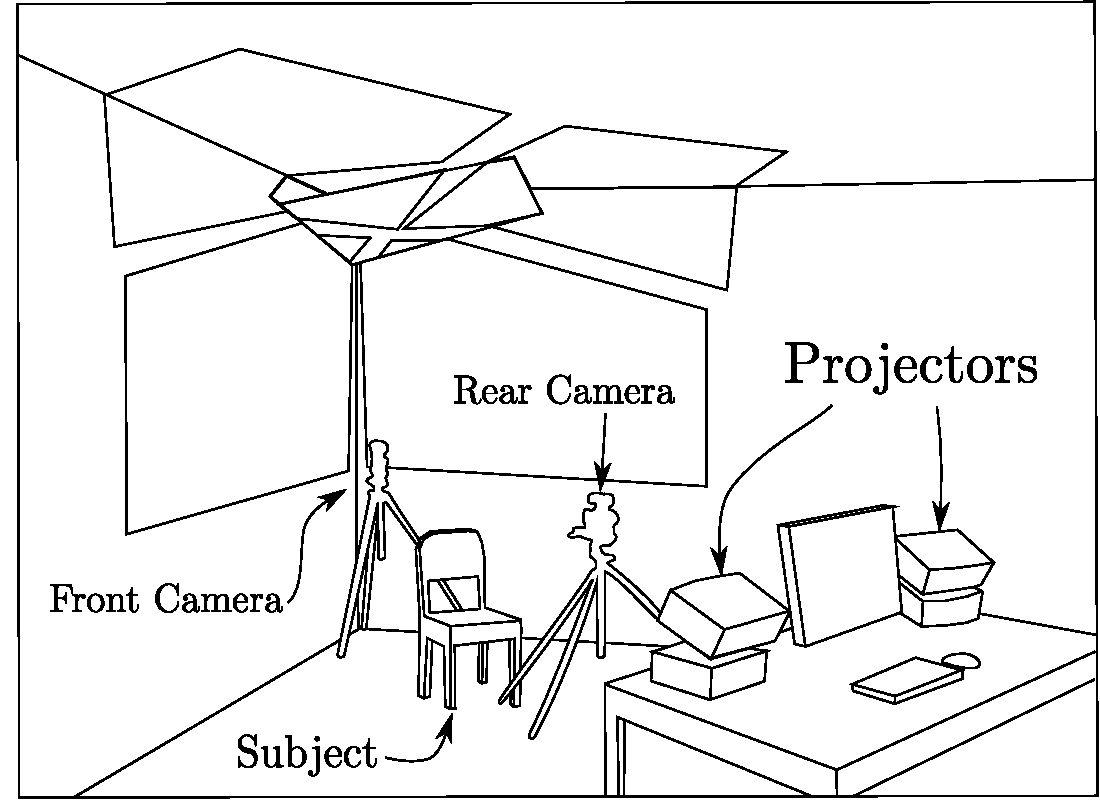
\includegraphics[height=2.5in]{figures_pami/camera_rig.pdf}
\caption{\small{\bf Training acquisition system:} Four projectors and two cameras controlled by one computer.}
\label{fig:system}
\end{figure}
With our projector system, our choice of illuminations is
constrained only by the need to achieve a good
SNR,\footnote{Since illuminations with more pixels illuminated
will have a better SNR (provided they don't saturate), there is
an engineering tradeoff between the SNR and the number of
training images.} avoid saturation, and achieve a reasonably
short acquisition time.  Two simplifying assumptions that we
make are that every pixel is either turned fully on or off in
every illumination, and that the illuminated regions do not
overlap.

Assuming that each pixel is fully on or off enables us to guarantee
that each illumination image has the same overall intensity, merely
by guaranteeing that we illuminate the same number of pixels in each image.\footnote{Since DLP projectors may have dramatically different response
curves depending on the mode they are in, it is not advisable to simply normalize each illumination image by its mean.}
Since our algorithm depends only on  the
linearity between the illuminations and the images, and not on the
relative intensities of the illuminations, the designer has the freedom to choose the overall intensity of the illuminations
to prevent saturation or low SNR, in a sort of offline exposure control.

Assuming that the sequentially illuminated regions do not overlap results in a
set of training images that span a larger cone than a similar number of
overlapping regions.  This results in training images that require fewer
negative coefficients in $\x$ to represent test images under natural
illuminations.  The effect of negative coefficients in $\x$ appears to depend
partly on how the test images are taken and is still under study.

{\em Relationship to existing work:} Most light stages used for face recognition have
been constructed for the purpose of creating public data sets to study
illumination invariance \cite{Georghiades2001-PAMI, Gross2008-FGR}.  Many other
light stages have been used for computer graphics purposes
\cite{debevec2000acquiring, jones2005performance}.
The light source can be
moved around manually \cite{masselus2002free}, but this may result in poor
consistency of illuminations between users.  Structured light applications use projectors to
directly illuminate the face (or other object) \cite{zhang2002rapid} for 3D
reconstruction, but this is very disturbing to the user.
Y.\ Schechner \cite{schechner2007multiplexing}
studies techniques for multiplexing illumination that can dramatically reduce the noise
of the demultiplexed images for certain classes of objects and cameras.
While these techniques have not been incorporated into the current
system, they fit elegantly into our framework and will likely be used
in future implementations.  We stress that use of this multiplexing technique
is independent from the choice of original (directional) illuminations.

\subsection{Choice of Illumination Patterns}

We ran two experiments to guide our choice of illuminations for
our large-scale experiments:
\begin{enumerate}
\item {\em Coverage Experiment.} In the first experiment we
    attempt to determine what coverage of the sphere is
    required to achieve good interpolation for test images.
    The subject was illuminated by 100 (50 front, 50 back)
    illuminations arranged in concentric rings centered at
    the front camera.  Subsets of the training images were
    chosen, starting at the front camera and adding a ring
    at a time.  Each time a ring was added to the training
    illumination set, the average $\ell^1$ registration
    error (residual) for a set of test images taken under
    sunlight was computed and plotted in Figure
    \ref{fig:illumination-patterns}(a).  The more rings of
    training illuminations are added, the lower the
    representation error becomes, with diminishing returns.
\item {\em Granularity Experiment.} In the second
    experiment we attempt to determine how finely divided
    the illumination sphere should be.  At the first
    granularity level, the projectors  illuminate the
    covered area uniformly.  At each subsequent granularity
    level each illuminated cell is divided in two along its
    longer side but intensity doubled.  For each
    granularity level the average $\ell^1$ registration
    error is computed as in the coverage experiment and
    shown in Figure \ref{fig:illumination-sufficiency}(b).
    Again, diminishing returns are observed as more
    illuminations are added.
\end{enumerate}
\begin{figure}
\centering
\begin{tabular}{cc}
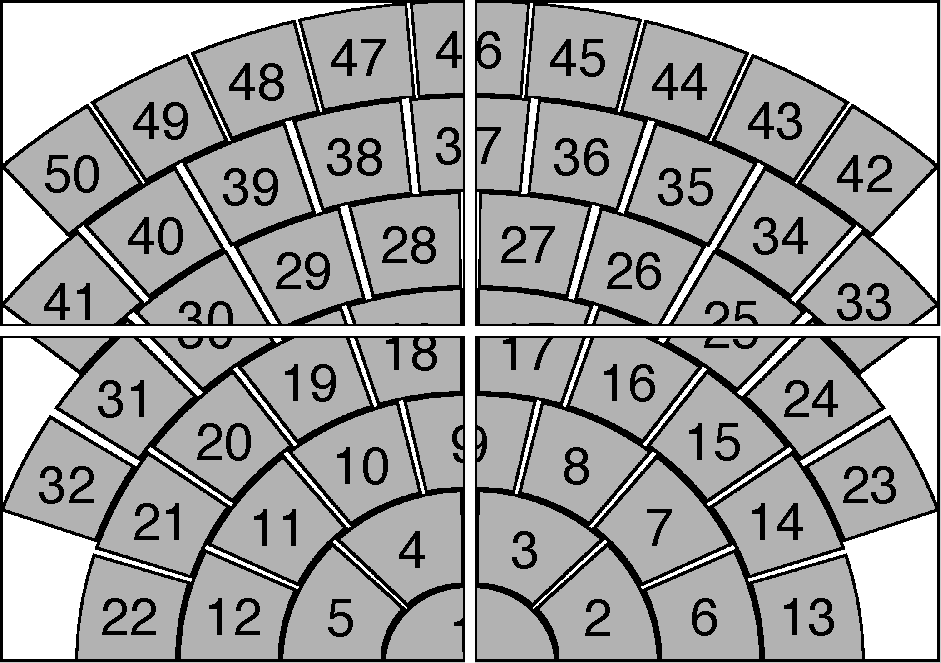
\includegraphics[height=1.7in]{figures_pami/coverage_experiment_asplode.png} &
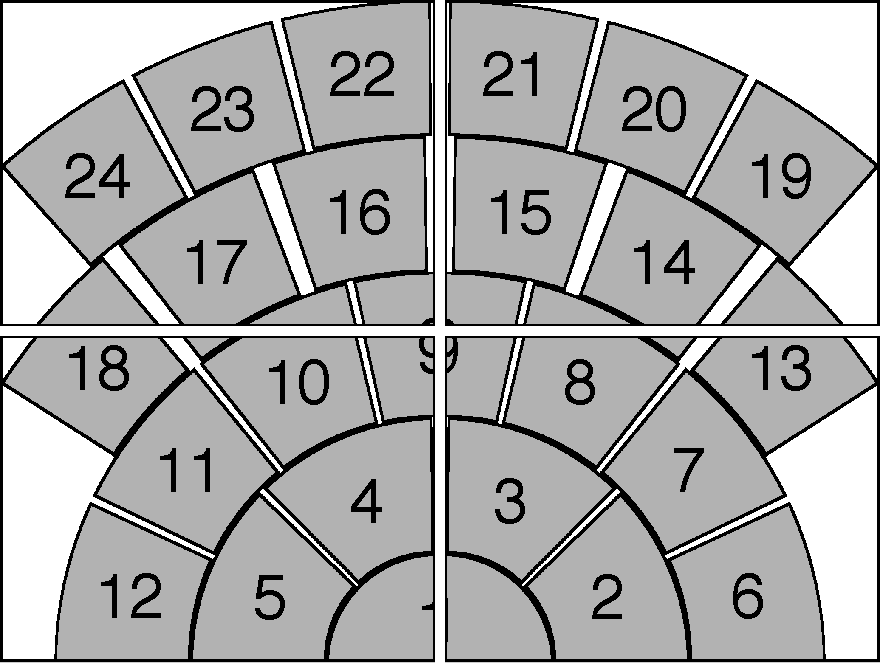
\includegraphics[height=1.7in]{figures_pami/final_cvpr_illuminations_asplode.png}  \\
(a) Coverage Experiment & (b) Chosen Illumination Patterns
\end{tabular}
\caption{\small{\bf Illumination Patterns.}   The cells are illuminated in sequence.  For rear illuminations the sequence is reversed.  In the chosen pattern's rear illumination, the cells 1-5 and 7-11 are omitted for a total of 38 illuminations. The four rectangular regions correspond to the four projectors.  }
\label{fig:illumination-patterns}
\end{figure}

\begin{figure}
\centering
\begin{tabular}{@{}c@{}c@{}}
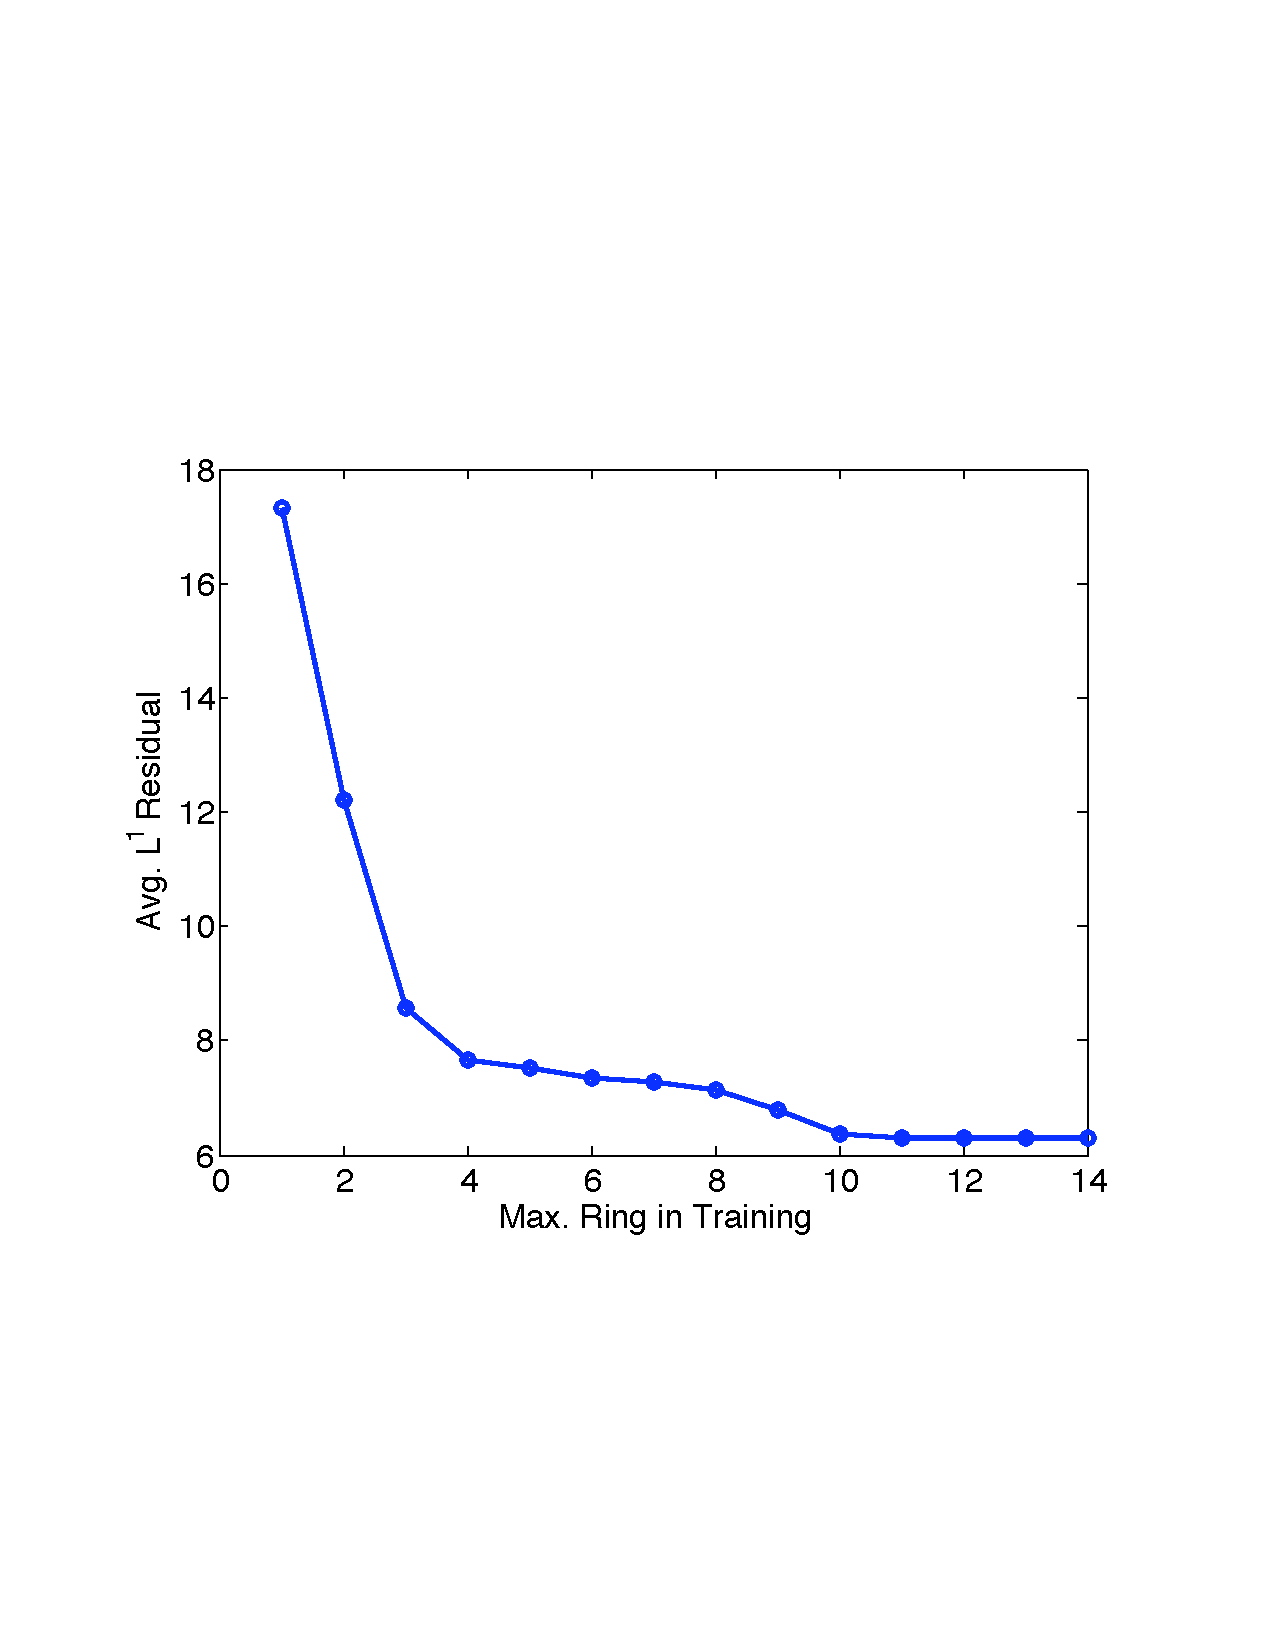
\includegraphics[height=2in]{figures_pami/illum_results/coverage_sunset.pdf} &
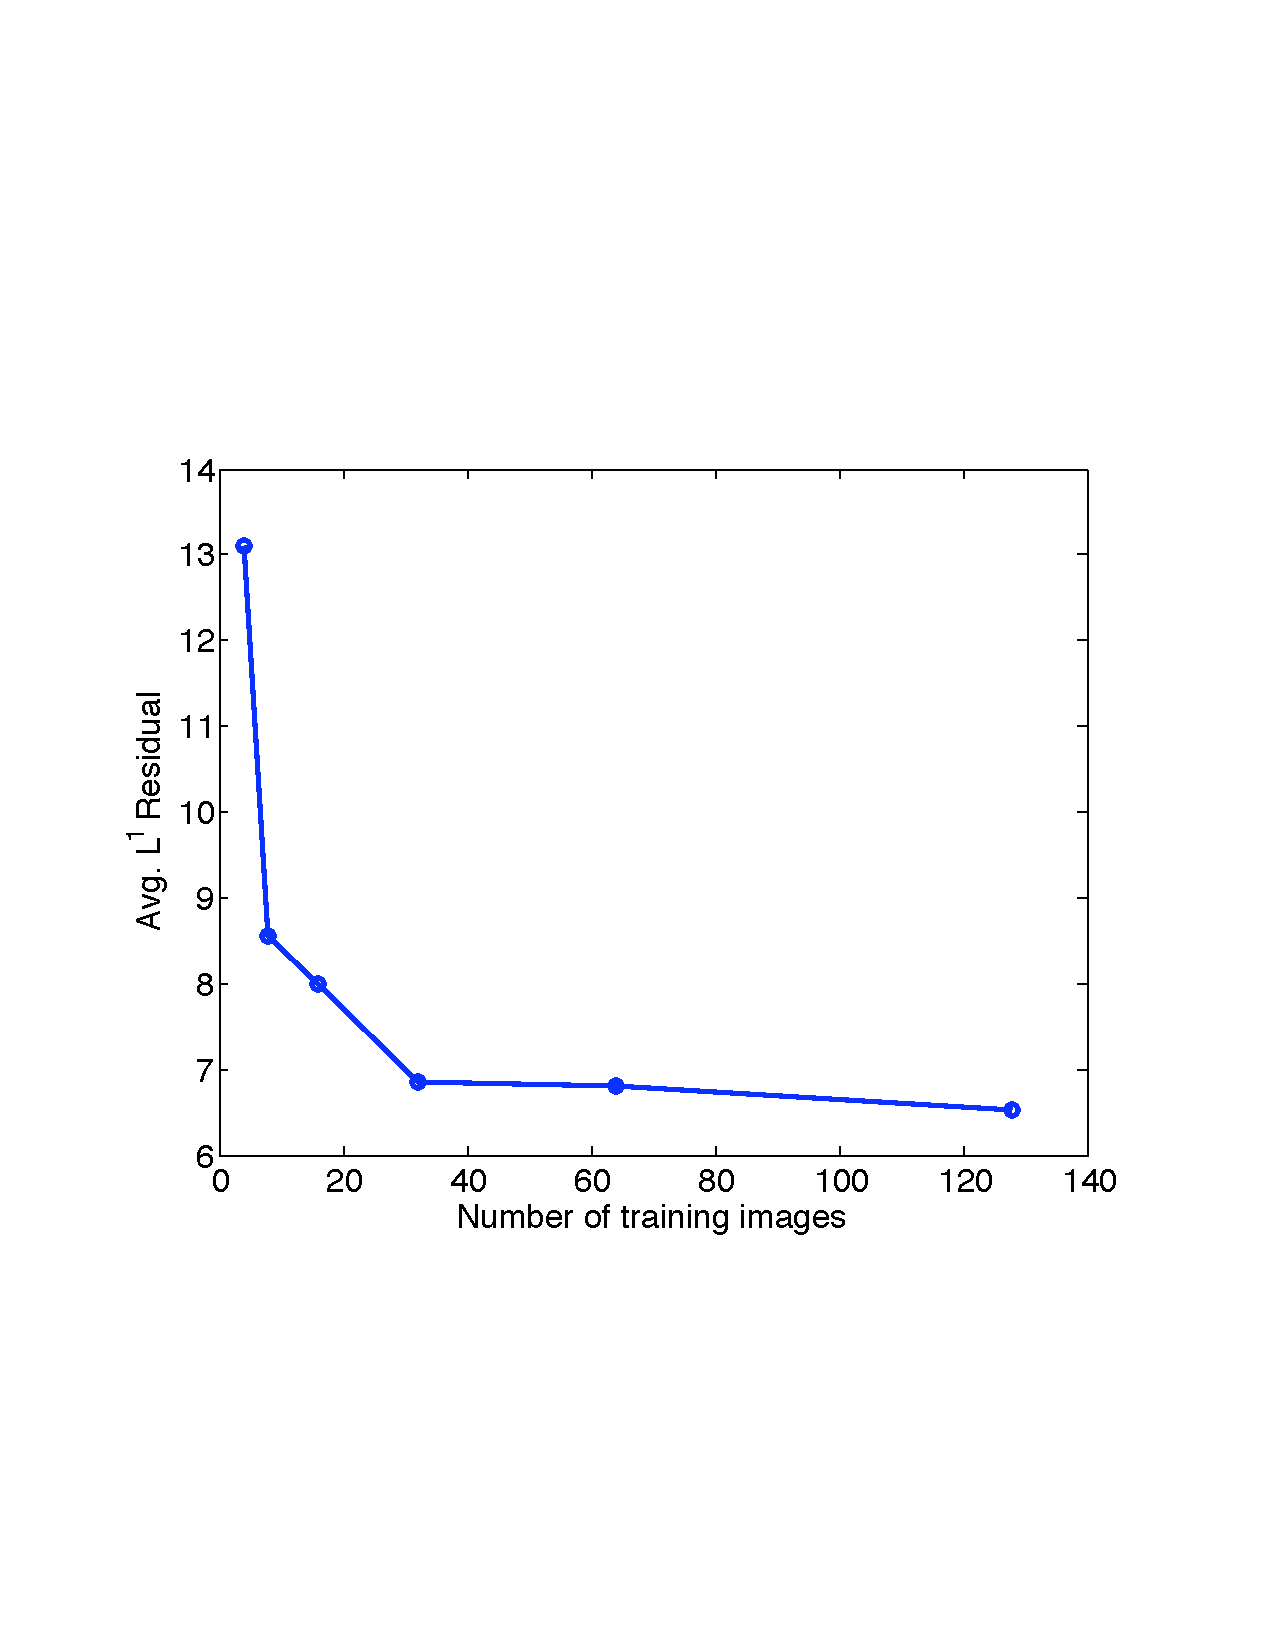
\includegraphics[height=2in]{figures_pami/illum_results/granularity_sunset.pdf} \\
(a) Coverage & (b) Granularity
\end{tabular}
\caption{\small{\bf Study of sufficient illuminations.} The average $\ell^1$ registration residual versus different illumination training sets. }
\label{fig:illumination-sufficiency}
\end{figure}

In the plot for the coverage experiment, Figure
\ref{fig:illumination-sufficiency}(a),
 we clearly see two plateau regions: one is after 4 rings
and one is after 10 rings. The first four rings represent the
typical frontal illuminations, which are present in most public
face datasets; however, we see that the residual stabilizes
after 10 rings which include some illuminations from the back
of the subject. This suggests that although the frontal
illuminations account for most of the illumination on the face,
some illuminations from the back are needed in the training set to
represent images with illumination coming from all directions.
In the plot for the granularity experiment, Figure
\ref{fig:illumination-sufficiency}(b), we observe that the
residual reaches a plateau after four divisions, corresponding
to a total of 32 illuminations. Based on the results from both
experiments, we decide to partition the area covered by the
first 10 rings into a total of 38 cells, whose layout is
explained in Figure \ref{fig:illumination-patterns}(b). For
our large-scale experiments, we have collected those
illuminations for all our subjects.\footnote{It is possible
that with further experimentation a reduced set of illuminations
can be found that performs as well or better.}

See below for the 38 training images of one subject:
\begin{figure}[h]
\centering
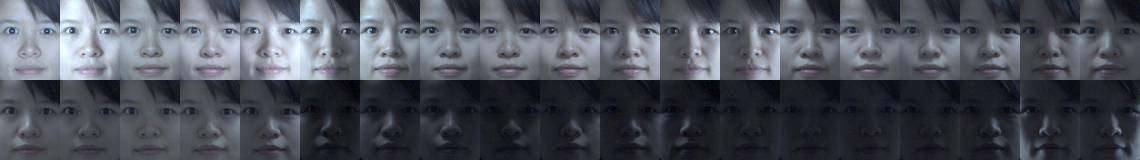
\includegraphics[width=\textwidth]{figures_pami/training.png}
\end{figure}


%\subsection{Should Positivity in the Representation Coefficients
%be Enforced?} One critical issue in linear illumination models
%is whether to enforce nonnegativity in the coefficients $\x$,
%i.e. whether to model illumination using a cone or a subspace.
%Some authors, i.e. \cite{Basri2003-PAMI}, have chosen to allow
%negative components in the coefficient vector $\x$ when
%representing one image as a sum of other images, and only
%enforce that the linear combination $A\x$ be positive
%everywhere.  Unfortunately, for non-convex objects such as
%faces, enforcing non-negativity of the representation is not
%sufficient to guarantee that the resulting image of the object
%is physical.  For example, consider a Lambertian planar object
%with a cylindrical hole drilled in it that is aligned with the
%optical axis of an orthographic camera.  Consider two images:
%one under illumination from a distant point source aligned with
%the hole, and one off of the hole axis.  Positively weighting
%the on-axis image and negatively weighting the on-axis image
%can result in an image where the bottom of the hole is more
%strongly illuminated than the surrounding plane.  The image is
%positive, but it is clearly non-physical.  It is worth
%emphasizing that this phenomenon is a result of some points on
%an object seeing a restricted subset of the illumination sphere
%(a violation of convexity),  and not a result of the
%directionality of the light chosen in the thought experiment.
%While the number of coefficients that actually end up negative
%after optimization is usually very small, we have observed
%pathological cases where the shadows next to the user's nose in
%the reconstructed image invert in value.

%Instead of using a smaller set of training images, allowing the
%coefficients to go negative to try to represent more test
%illuminations, and risking over-fitting, we decided to enforce
%non-negativity of the coefficients.  Nonnegative combinations
%of images are guaranteed to correspond to physically plausible
%images.  all physical illuminations unless the training images
%actually span the boundary of the illumination cone. Because we
%have a flexible acquisition system, we can directly generate a
%set of illuminations that span most of the illumination cone,
%without resorting to negative coefficients and risking
%overfitting.  Thus, in Algorithm 1, we have enforced that the
%coefficients $\x$ be non-negative.

%One of the main factors that complicates face recognition, and computer vision in general, is that two images of the same person's face can be very different, even if the pose is carefully controlled and all points on the person's face are visible in both images.  The most safe, reliable, and general assumption that can be made about the imaging process is that it is linear with respect to the intensity of different light sources.  The set of images of a given object is therefore a cone in the non-negative orthant of the pixel basis.  All recognition algorithms that rely on vision for training rely on images sampled from this cone.


\section{Tests on Public Databases}\label{sec:multipie}
In this section and the next section, we conduct comprehensive experiments on
large-scale face databases to verify the performance of our algorithm and
system. We first test on the largest public face database available that is
suitable for testing our algorithm, the CMU Multi-PIE.  One shortcoming of the
CMU Multi-PIE database for our purposes is that there is no separate set of
test images taken under natural illuminations; we are left to choose which sets
of images to use for testing and training.  To challenge our algorithm, we
choose only a small set of illuminations for the training set, yet we include
all illuminations in the testing set. In the following section, we will test
our algorithm on a face dataset that is collected by our own system. The goal
for that experiment will be to show that with a sufficient set of training
illuminations for each subject, our algorithm indeed works stably and robustly
with practical illumination, misalignment, pose, and occlusion, as already
indicated by our experiment shown in Figure \ref{fig:promo}(bottom).

CMU Multi-PIE provides the most extensive test set among public
datasets. This database contains images of 337 subjects across
simultaneous variation in pose, expression, and illumination.
Of these 337 subjects, we use all of the 249 subjects present
in Session 1 as the training set. The remaining 88 subjects are
treated as ``impostors'', or invalid images. For each of the
249 training subjects, we include frontal images of 7 frontal
illuminations,\footnote{They are illuminations
$\{0,1,7,13,14,16,18\}$ of \cite{Gross2008-FGR}. For each
directional illumination, we subtract the ambient-illuminated
image 0.} taken with neutral expression. As suggested by the
work of \cite{Georghiades2001-PAMI}, we choose these extreme
frontal illuminations in the hope that they would linearly
represent other frontal illuminations well. For the test set,
we use all 20 illuminations from Sessions 2-4, which were
recorded over a period of several months. The dataset is
challenging due to the large number of subjects, and due to
natural variation in subject appearance over time.
Table \ref{tab:MultiPIE-recognition2} shows the result of our
algorithm on each of the 3 testing sessions. Our algorithm
achieves recognition rates above $90\%$ for all three sessions.
For the test images, our iterative alignment was initialized
automatically via the Viola and Jones' face detector. To
demonstrate that the sparse representation based recognition
step is indeed beneficial even when there are no impostors, we
include results for recognition based only on the alignment
error residuals (i.e. $S=1$), shown in row 1.

\begin{table}
\caption{Recognition rates on the Multi-PIE database for
Algorithm 1 and \cite{Yang2010-CVPR}}
\centerline{
\begin{tabular}{|c|c|c|c|c| }
\hline
Recognition rate & Session 2 & Session 3 & Session 4  \\
\hline
{Alg. 1, $S=1$} & 90.7\% & 89.6\% & 87.5\% \\
\hline
{Alg. 1} & 93.9\% & 93.8\% & 92.3\% \\
\hline
{Alg. 1 with improved window} & 95.0\% & {\bf 96.3}\% & {\bf 97.3}\% \\
\hline
\cite{Yang2010-CVPR} & {\bf 95.2}\% & 93.4\% & 95.1\% \\
\hline
\end{tabular}
\label{tab:MultiPIE-recognition2} }
\end{table}

\newcommand{\tempwidth}[0]{0.9in}
\begin{figure}
\centering
{
\begin{tabular}{@{}c@{}c@{}c@{}c@{}c@{}c@{}}
\hspace{-2mm}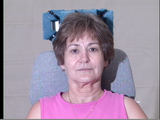
\includegraphics[width=\tempwidth,clip=true]{figures_pami/multipie_failed/079_01_01_051_08.png}  &
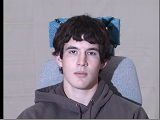
\includegraphics[width=\tempwidth,clip=true]{figures_pami/multipie_failed/111_01_01_051_08.png}  &
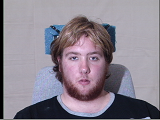
\includegraphics[width=\tempwidth,clip=true]{figures_pami/multipie_failed/196_01_01_051_08.png}  &
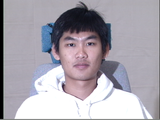
\includegraphics[width=\tempwidth,clip=true]{figures_pami/multipie_failed/130_01_01_051_08.png}  &
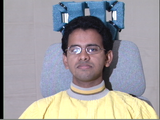
\includegraphics[width=\tempwidth,clip=true]{figures_pami/multipie_failed/163_01_01_051_08.png}  &
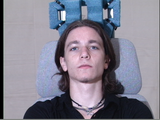
\includegraphics[width=\tempwidth,clip=true]{figures_pami/multipie_failed/175_01_01_051_08.png} \\
\hspace{-2mm}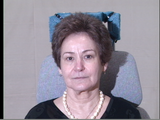
\includegraphics[width=\tempwidth,clip=true]{figures_pami/multipie_failed/079_02_01_051_08.png}  &
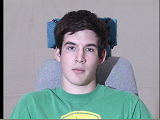
\includegraphics[width=\tempwidth,clip=true]{figures_pami/multipie_failed/111_02_01_051_08.png}  &
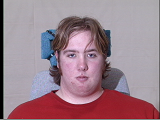
\includegraphics[width=\tempwidth,clip=true]{figures_pami/multipie_failed/196_02_01_051_08.png}  &
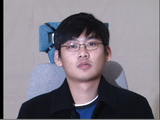
\includegraphics[width=\tempwidth,clip=true]{figures_pami/multipie_failed/130_02_01_051_08.png}  &
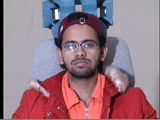
\includegraphics[width=\tempwidth,clip=true]{figures_pami/multipie_failed/163_02_01_051_08.png}  &
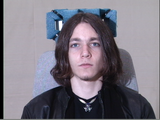
\includegraphics[width=\tempwidth,clip=true]{figures_pami/multipie_failed/175_02_01_051_08.png} \\
\hspace{-2mm}(a) & (b) & (c) & (d) & (e) & (f) 
\end{tabular}
}
\caption{\small{\bf Representative failures from Multi-PIE}. {\bf Top:} training from Session 1; {\bf Bottom:} test images from Session 2. Due to changes in hair, glasses, beard, or pose, our alignment fails on these subjects regardless of test image illumination.}
\label{fig:failed-examples}
\end{figure}
\subsection{Improving the Sampling Window}
Our algorithm's errors are mostly caused by a few subjects who
significantly change their appearances between sessions (such
as hair, facial hair, and eyeglasses). Some representative
examples are shown in Figure \ref{fig:failed-examples}. For those subjects, alignment and recognition fail on
almost all test illuminations.
\begin{figure}[b]
\centering
{
\begin{tabular}{@{}cc@{}}
\includegraphics[trim=1.9in .7in 1.9in .5in, clip, height=1.8in]{figures_pami/example.png} &
\includegraphics[trim=1.9in .7in 1.9in .5in, clip, height=1.8in]{figures_pami/example_new.png} \\
Default window. & Proposed window.
\end{tabular}
}
\caption{\small{\bf Choosing different sampling windows.}}
\label{fig:new-mask}
\end{figure}
Meanwhile, this observation also suggests that we might be able
to improve the performance of our method by carefully choosing
a face region which is less affected by the above factors for
recognition. In particular, since the forehead region is likely
to be affected by the change of hair style, we try replacing
the previous $80 \times 60$ canonical frame with a new
window that better excludes the forehead. We adjust the
resolution of the window to keep $m$ approximately constant. In addition,
we cut off two lower corners of the $80 \times 60$ canonical frame, motivated by
the observation that in many cases the corners
actually contain background. An example of the new window
is shown in Figure~\ref{fig:new-mask}.

\begin{table*}
\centering
\small
\caption{\small Recognition rates on the Multi-PIE database for
different pairings of alignment and recognition stages.}
\centerline{
\begin{tabular}{|c|c|c|c|c|c|c|c|c|c|c| }
\hline
\backslashbox{Rec.}{Align.}
& \multicolumn{3}{|c|}{Face Detector}
& \multicolumn{3}{|c|}{Manual}
& \multicolumn{3}{|c|}{Iterative Alignment}
\\
\hline
Session $\rightarrow$	& 2		&3			&4			& 2		&3			&4			& 2		&3			&4		\\
\hline
NS	& 30.8\%	& 29.4\%	& 24.6\%	& 77.6\%	& 74.3\%	& 73.4\%	& 84.5\%	& 82.3\%	& 81.4\% \\
\hline
NN	& 26.4\%	& 24.7\%	& 21.9\%	& 67.3\%	& 66.2\%	& 62.8\%	& 73.5\%	& 69.6\%	& 69.3\% \\
\hline
LDA	& 5.1\%		& 5.9\%		& 4.3\%		& 49.4\%	& 44.3\%	& 47.9\%	& 91.0\%	& 89.9\%	& 88.1\% \\
\hline
LBP	& 39.9\%	& 38.1\%	& 33.9\%	& 93.3\%	& 91.2\%	& 92.9\%	& {\bf 95.2\%}	& {\bf 94.7\%}	& {\bf 93.5\%} \\
\hline
SRC	& -- & -- & -- & -- & -- & -- & 93.9\%	& 93.8\%	& 92.3\% \\
\hline
\end{tabular}
\label{tab:MultiPIE-recognition} }
\end{table*}

Table \ref{tab:MultiPIE-recognition2} shows that the
recognition rates on Multi-PIE indeed increase with this new
window. In addition, Figure \ref{fig:failed-examples}(a), (b),
and (c) illustrate three representative subjects for which the
recognition rates of our algorithm are significantly boosted
with the new window. However, we should mention that the best
choice of the window is problem-specific and there is not a
simple guideline to follow. For example, although the new
window performs better on Multi-PIE, the same window does not
help at all on our own database, which will be introduced in
the next section. This is because most of the training and
testing images in our database are taken on the same day so the
variation in hair style is very small. Hence, excluding the
forehead part may actually result in loss of useful
discriminative information.

\subsection{Comparison to Existing Work}

We first compare our result to the recent work
\cite{Yang2010-CVPR}. Notice that in \cite{Yang2010-CVPR}, the
initial registration is obtained from manually selected outer
eye corners. Then, a supervised hierarchical sparse coding
model based on local image descriptors is trained, which enjoys
certain translation invariant properties. With the same
training and testing sets, \cite{Yang2010-CVPR} is able to
handle the remaining misalignment and achieves state-of-the-art
performance on the CMU Multi-PIE database.
Table~\ref{tab:MultiPIE-recognition2} shows that our algorithm
achieves similar or better performance on different sessions of
Multi-PIE.

% Classical algorithms
To better examine the effectiveness of our iterative alignment
algorithm, we next compare our result to baseline
linear-projection-based algorithms, such as Nearest Neighbor
(NN), Nearest Subspace (NS) \cite{Lee2005-PAMI}, and Linear
Discriminant Analysis (LDA)
\cite{Belhumeur1997-PAMI}.\footnote{We do not list results on
PCA \cite{Turk1991-CVPR} as its performance is always below
that of Nearest Subspace.} Since these algorithms assume
pixel-accurate alignment, they are not expected to work well if
the test image is not well aligned with the training. In
Table~\ref{tab:MultiPIE-recognition}, we report the results of
these classical algorithms with three types of testing image
alignment: 1.\ alignment from the Viola and Jones' detector,
2.\ alignment via manually selected outer eye
corners,\footnote{Two manually clicked points are sufficient to
define a similarity transformation. All of the experiments in
this section are carried out with similarity transformations.}
and 3.\ the output of our iterative alignment algorithm. The
performance drop of the LDA algorithm on Multi-PIE reported
here seems to agree with that reported already in
\cite{Gross2008-FGR}.  All of the classical algorithms benefit
greatly from being paired with our iterative alignment
algorithm.

% LBP
We also compare our result to Local Binary Patterns (LBP)
\cite{Ahonen2006-PAMI}, a local appearance descriptor which is
able to capture fine details of facial appearance and texture.
Due to its robustness to variations in illumination, facial
expression, aging and other changes, LBP has achieved the
state-of-the-art face recognition performance in the scenario
when only one sample per person is used for training
\cite{Tan06facerecognition}. In this section, we follow the same
steps as in \cite{Ahonen2006-PAMI} to construct an LBP
descriptor for each training and testing sample. The $80\times
60$ face region is first divided into a regular $10\times 10$
grid of cells, each of size $8\times 6$ pixels. Within each
cell, the histogram of 59 uniform binary patterns is then
computed, where the patterns are generated by thresholding 8
neighboring pixels in a circle of radius 2 using the central
pixel value. Finally, the local histograms are concatenated to
produce the global descriptor vector. As suggested in
\cite{Ahonen2006-PAMI}, the recognition is performed using a
nearest neighbor classifier with Chi square distance as the
distance measure and we report the recognition rates with the
same three types of input as before.

As shown in Table~\ref{tab:MultiPIE-recognition}, although LBP
achieves competitive recognition rates given manually aligned
training and testing samples, demonstrating its robustness to
moderate misalignment, it still benefits from using the output
of our iterative alignment algorithm as the input. In addition,
like the other classical algorithms, the performance of LBP
degrades dramatically if it is applied directly to the output
of a face detector. This is notable given that LBP is often
applied without any special alignment in practice. Finally, we
attribute the improvement in performance of LBP over SRC in
this experiment to its robustness to illumination components
that cannot be linearly interpolated by the training set.

In addition, although our algorithm is not designed for
recognition when there is only a single gallery image per user,
we compare its performance with LBP within this setting for
completeness. For this experiment, we use the FERET dataset
\cite{phillips1998feret}, which contains five standard
partitions: `fa' is the gallery containing 1196 frontal images
of 1196 subjects, and `fb', `fc', `dup1' and `dup2' are four
sets of probe images. The testing sets differ from the training
in facial expression (`fb'), illumination (`fc'), aging (`dup1'
) and long aging (`dup2'). In fact, except for `fb', we notice
significant changes of illumination in all the other three test
sets. For the training, we again crop and normalize the face
region from each original image to an $80\times 60$ window
using manually marked eye coordinates \cite{Deng2010-PR}. In
Table~\ref{tab:FERET-recognition}, we report the performance of
our algorithm on the four test sets, with input directly
obtained from the Viola and Jones' detector. We also report the
performance of LBP with the same three types of input as before:
we use letters
``$d$'', ``$m$'', and ``$i$'' to indicate face detector, manual
alignment, and our iterative alignment algorithm, respectively.

As expected, our algorithm does not perform well except for
`fb', in which the illumination is similar to the training and
the mere variation in facial expression is handled well by the
sparse error model. For the other three test sets, our
algorithm fails because the illumination changes and other
variations seriously violate the assumptions of our method.
This also explains why LBP performs worse with our iterative
alignment algorithm, compared to manual alignment. On the other
hand, while LBP achieves the best recognition rates given
manually aligned training and testing samples, its performance
degrades drastically when the input is obtained directly from
the face detector. It is also worth noting that similar poor
performance of LBP, as well as other descriptors, has been
observed on the Labeled Face in the Wild (LFW) database, where
the training is uncontrolled and limited and the input is
directly obtained from the face detector \cite{Wolf2008-ECCV}.
\begin{table}
\caption{Performance on single gallery image FERET dataset}
\centerline{
\begin{tabular}{|c|c|c|c|c| }
\hline
Recognition rate \% & fb & fc & dup1 & dup2 \\
\hline
$LBP_d$ & 54.8 & 10.3 & 29.8 & 19.8 \\
\hline
$LBP_m$ & {\bf 96.6} & {\bf 58.8} & {\bf 71.6} & {\bf 61.5} \\
\hline
$LBP_i$ & 94.5 & 42.8 & 46.5 & 21.1 \\
\hline
{Alg. 1} & 95.2 & 28.4 & 46.1 & 20.3 \\
\hline
\end{tabular}
\label{tab:FERET-recognition} }
\end{table}

All of these experimental results confirm that
both illumination and alignment need to be simultaneously handled
well in order to achieve accurate face recognition, even when there is
no obvious occlusion or corruption in the test.

\subsection{Subject Validation}

We test the algorithms' ability to reject invalid images of the
88 subjects not appearing in the training database. As
mentioned before, the \emph{sparsity concentration index} (SCI)
is used as the outlier rejection rule. Given the sparse
representation $\x$ of a test image with respect to $K$
training classes, the SCI measures how concentrated the
coefficients are on a single class in the dataset and is
defined as in \cite{Wright2009-PAMI}:
\begin{displaymath}
\textup{SCI}(\x) \doteq \frac{K \cdot \max_i \|\delta_i(\x)\|_1 /
\|\x\|_1 - 1}{K - 1} \in [0,1] .
\end{displaymath}
It is easy to see that if $\textup{SCI}(\x) = 1$, the test
image is represented using images from one single subject
class; if $\textup{SCI}(\x) = 0$, the coefficients are spread
evenly over all classes. Thus, we can choose a threshold $t \in
[0,1]$ for the proposed method and accept a test image as valid
if $\textup{SCI}(\x) \geq t$, and otherwise reject it as
invalid. We compare this classifier to classifiers based on
thresholding the error residuals of NN, NS, LDA, and LBP.
\begin{figure}[t]
{
\centerline{
\begin{tabular}{@{}cc@{}}
\includegraphics[height=2.5in]{figures_pami/pami_roc_revision2} &
\includegraphics[height=2.5in]{figures_pami/pami_roc2} \\
(a) & (b) \\
\end{tabular}
}}
\caption{\small {\bf ROC curves} for subject validation on Multi-PIE database,
(a) for all algorithms with iterative alignment, and
(b) for the classical algorithms with manual alignment (indicated by a subscript ``m'').}\label{fig:roc-multipie}
\end{figure}

Figure \ref{fig:roc-multipie} plots the receiver operating
characteristic (ROC) curves, which are generated by sweeping
the threshold $t$ through the entire range of possible values
for each algorithm.\footnote{Rejecting invalid images not in
the entire database is much more difficult than deciding if two
face images are the same subject. Figure \ref{fig:roc-multipie}
should not be confused with typical ROC curves for face
similarity, e.g., \cite{PhillipsP2007}.} On the left we can see
that the SCI based recognition approach significantly
outperforms the other algorithms, including LBP, even when all
algorithms are coupled with our proposed iterative alignment.
In the right plot we again see that classical algorithms, and
even LBP, are very sensitive to alignment.  Similar contrasts
between our algorithm and baseline algorithms were also
observed for SRC in \cite{Wright2009-PAMI}, though on much
smaller datasets.

\subsection{Recognition with Synthetic Random Block Occlusion}

We further test the robustness of our $\ell^1$-norm based
algorithm to synthetic occlusion. We simulate various levels of
occlusion from 10\% to 50\% by replacing a randomly located
block of the face image with an image of a baboon, as shown in
Figure~\ref{fig:multipie-occ-rec}. In this experiment, to avoid
any other factors that may contribute to extra occlusion of the
face (such as the change of hair style), we choose illumination
10 from Session 1\footnote{This is the same session as the
training set.} as testing. The rest of the experimental setting
remains unchanged. The table in
Figure~\ref{fig:multipie-occ-rec} shows that our algorithm is
indeed capable of handling a moderate amount of occlusion. For
example, at 20\% occlusion, our algorithm still achieves 94.9\%
recognition rate.

\renewcommand{\tempwidth}{0.2\textwidth}
\begin{figure}
\centering
\begin{tabular}{@{}c@{}c@{}c@{}c@{}c@{}}
\includegraphics[width=\tempwidth,clip=true]{figures_pami/multipie_occ/occ10.png} &
\includegraphics[width=\tempwidth,clip=true]{figures_pami/multipie_occ/occ20.png} &
\includegraphics[width=\tempwidth,clip=true]{figures_pami/multipie_occ/occ30.png} &
\includegraphics[width=\tempwidth,clip=true]{figures_pami/multipie_occ/occ40.png} &
\includegraphics[width=\tempwidth,clip=true]{figures_pami/multipie_occ/occ50.png}  \\
\end{tabular}
\caption{\small{\bf Recognition under varying level of
random block occlusion.} The above row of images shows examples of occluded test images with occlusion level from 10\% to 50\%. Our method maintains high recognition rates up to 30\% occlusion:}
{
\begin{tabular}{|c|c|c|c|c|c| }
\hline
Percent occluded & 10\% & 20\% & 30\% & 40\% & 50\%  \\
\hline
Recognition rate & 99.6\% & 94.9\% & 79.6\% & 46.5\% & 19.8\% \\
\hline
\end{tabular}
}
\label{fig:multipie-occ-rec}
\end{figure}

\subsection{Recognition with Pose and Expression} We now run tests of
our algorithm on a subset of the images from Multi-PIE with pose and expression variation in the test set, although we do not model these variations explicitly.
Using the same training set as above, we test our algorithm on
images in Session 2 with $15^\circ$ pose, for all 20
illuminations. As expected, the recognition rate drops to 78.0\%. We also test our
algorithm on images in Session 3 with smile, again for all 20
illuminations. The recognition rate is 64.8\%. Of course, it is reasonable to expect that
the performance of our method will be significantly improved if pose and expression data
are available in the training.


\section{Tests on Our Own Database}\label{sec:own-data} Using the training acquisition
system we described in Section \ref{sec:illumination}, and shown in Figure
\ref{fig:system}, we have collected the frontal view of 109
subjects {\em without eyeglasses} under 38 illuminations shown
in Figure \ref{fig:illumination-patterns}. For testing our
algorithm, we have also taken 935 images of these subjects with
a different camera under a variety of practical conditions.

\subsection{Necessity of Rear Illuminations} To see how
training illuminations affect the performance of our algorithm
in practice, we now compare how well a few frontal
illuminations can linearly represent: 1. other frontal illuminations
taken under the same laboratory conditions, and 2. typical
indoor and outdoor illuminations. To this end, we use the face
database acquired by our system and use 7 illuminations per
subject as training. The illuminations are chosen to be similar
to the 7 illuminations used in the previous experiment on
Multi-PIE.\footnote{We use the illuminations $\{6, 9, 12,
13, 18, 21, 22\}$ shown in Figure
\ref{fig:illumination-patterns}(b) to mimic the illuminations
 $\{0, 1, 6, 7, 13, 14, 18\}$ in Multi-PIE.} We then test
our algorithm on the remaining $24 - 7 = 17$ frontal
illuminations for all the subjects. The recognition rate is
$99.8\%$, nearly perfect. We also test our algorithm on 310
indoor images and 168 outdoor images of these subjects taken
under a variety of lighting conditions (category 1 and 2
specified below), similar to the one shown in Figure
\ref{fig:promo}, and the recognition rates for indoor and
outdoor images drop down to $94.2\%$ and $89.2\%$,
respectively. This is a strong indication that
frontal illuminations taken under laboratory conditions
are insufficient for representing test images under typical indoor and
outdoor illuminations.

\renewcommand{\tempwidth}{0.1667\textwidth}
\begin{figure}
\centering
\begin{tabular}{@{}c@{}c@{}c@{}c@{}c@{}c@{}}
\includegraphics[width=\tempwidth,clip=true]{figures_pami/uiuc_example/normal_indoor/DSC_1318.JPG} &
\includegraphics[width=\tempwidth,clip=true]{figures_pami/uiuc_example/normal_indoor/DSC_1521.JPG} &
\includegraphics[width=\tempwidth,clip=true]{figures_pami/uiuc_example/normal_indoor/DSC_1673.JPG} &
\includegraphics[width=\tempwidth,clip=true]{figures_pami/uiuc_example/normal_indoor/DSC_1732.JPG} &
\includegraphics[width=\tempwidth,clip=true]{figures_pami/uiuc_example/normal_indoor/DSC_1941.JPG} &
\includegraphics[width=\tempwidth,clip=true]{figures_pami/uiuc_example/normal_indoor/DSC_3766.JPG} \\
\includegraphics[width=\tempwidth,clip=true]{figures_pami/uiuc_example/normal_outdoor/DSC_1574.JPG} &
\includegraphics[width=\tempwidth,clip=true]{figures_pami/uiuc_example/normal_outdoor/DSC_1622.JPG} &
\includegraphics[width=\tempwidth,clip=true]{figures_pami/uiuc_example/normal_outdoor/DSC_1641.JPG} &
\includegraphics[width=\tempwidth,clip=true]{figures_pami/uiuc_example/normal_outdoor/DSC_3522.JPG} &
\includegraphics[width=\tempwidth,clip=true]{figures_pami/uiuc_example/normal_outdoor/DSC_3707.JPG} &
\includegraphics[width=\tempwidth,clip=true]{figures_pami/uiuc_example/normal_outdoor/DSC_3772.JPG} \\
\includegraphics[width=\tempwidth,clip=true]{figures_pami/uiuc_example/glasses/DSC_1397.JPG} &
\includegraphics[width=\tempwidth,clip=true]{figures_pami/uiuc_example/glasses/DSC_1532.JPG} &
\includegraphics[width=\tempwidth,clip=true]{figures_pami/uiuc_example/glasses/DSC_1556.JPG} &
\includegraphics[width=\tempwidth,clip=true]{figures_pami/uiuc_example/glasses/DSC_1585.JPG} &
\includegraphics[width=\tempwidth,clip=true]{figures_pami/uiuc_example/glasses/DSC_1688.JPG} &
\includegraphics[width=\tempwidth,clip=true]{figures_pami/uiuc_example/glasses/DSC_4035.JPG} \\
\end{tabular}
\caption{\small{\bf Representative examples of categories C1-C3}. One row for each category.}\label{fig:examples1-3}
\end{figure}

\begin{figure}[t]
\centering
\begin{tabular}{@{}c@{}c@{}c@{}c@{}c@{}c@{}}
\includegraphics[width=\tempwidth,clip=true]{figures_pami/uiuc_example/sunglasses/DSC_1565.JPG} &
\includegraphics[width=\tempwidth,clip=true]{figures_pami/uiuc_example/sunglasses/DSC_3656.JPG} &
\includegraphics[width=\tempwidth,clip=true]{figures_pami/uiuc_example/sunglasses/DSC_3827.JPG} &
\includegraphics[width=\tempwidth,clip=true]{figures_pami/uiuc_example/sunglasses/DSC_4090.JPG} &
\includegraphics[width=\tempwidth,clip=true]{figures_pami/uiuc_example/sunglasses/DSC_4106.JPG} &
\includegraphics[width=\tempwidth,clip=true]{figures_pami/uiuc_example/sunglasses/DSC_4126.JPG} \\
\includegraphics[width=\tempwidth,clip=true]{figures_pami/uiuc_example/sunglasses_failed/DSC_1611.JPG} &
\includegraphics[width=\tempwidth,clip=true]{figures_pami/uiuc_example/sunglasses_failed/DSC_3528.JPG} &
\includegraphics[width=\tempwidth,clip=true]{figures_pami/uiuc_example/sunglasses_failed/DSC_3744.JPG} &
\includegraphics[width=\tempwidth,clip=true]{figures_pami/uiuc_example/sunglasses_failed/DSC_3995.JPG} &
\includegraphics[width=\tempwidth,clip=true]{figures_pami/uiuc_example/sunglasses_failed/DSC_4030.JPG} &
\includegraphics[width=\tempwidth,clip=true]{figures_pami/uiuc_example/sunglasses_failed/DSC_4095.JPG} \\
\end{tabular}
 \caption{\small{\bf Representative examples of category C4}. Top row: successful examples with our method using overlapping blocks. Bottom row: failures with our method using overlapping blocks.}\label{fig:examples4}
\end{figure}

\subsection{Large-Scale Test with Sufficient Training
Illuminations} Now we use all 109 subjects and 38 illuminations
in the training and test on 935 images taken under a variety of
practical illuminations and conditions. We have manually partitioned the test images into four main
categories:
\begin{description}
\item[C1:] 310 \emph{indoor} images of 72 subjects without
    eyeglasses, frontal view
    (Fig.~\ref{fig:examples1-3}, row 1).
\item[C2:] 168 \emph{outdoor} images of 48 subjects without
    eyeglasses, frontal view
    (Fig.~\ref{fig:examples1-3}, row 2).
\item[C3:] 211 images of 32 subjects with \emph{eyeglasses}
    (Fig.~\ref{fig:examples1-3}, row 3).
\item[C4:] 246 images of 56 subjects with \emph{sunglasses}
    (Fig.~\ref{fig:examples4}).
\end{description}
We apply Viola and Jones' face detector on these images and
directly use the detected faces as the input to our algorithm.
Table~\ref{tab:UIUC-recognition} reports the performance of our
algorithm on each category.
Since our focus is on face
recognition, the errors do not include failures of the face
detector on some of the more challenging images.
As one can see, our algorithm achieves higher than 95\%
recognition rates on categories 1-3. Furthermore, using the
full set of 38 illuminations indeed improves the performance of
our system under practical illumination conditions compared to
only using a small subset of 7 illuminations. However, the
performance dramatically drops when the faces are occluded by
various types of sunglasses, which could cover up to 40\% of
the entire face. Given the previous experimental results on
synthetic random block occlusions, and given that the
illuminations are more challenging, the result is not
surprising. In the next subsection, we will show how additional
assumptions can be used to improve the recognition performance.
\begin{table}[h]
\centering \caption{Recognition rates on our own
database.}
\begin{tabular}{|c|c|c|c|c| }
\hline
Test Category & C1 & C2 & C3 & C4  \\
\hline
\hline
Recognition Rate & 98.4\% & 95.8\% & 95.1\% & 40.9\% \\
\hline
\end{tabular}
\label{tab:UIUC-recognition}
\end{table}

\subsection{Improving the Performance with Occlusion using Overlapping Blocks}
A traditional approach to improve the performance of face
recognition under severe occlusion is to use subregions instead
the entire face as a whole. This idea has been explored in many
earlier works; see \cite{Pentland1994-CVPR, Wright2009-PAMI}
for examples. Since in most real world cases the occlusion is contiguous, it is reasonable to argue that a minority of the
subregions are likely to be affected by the occlusion. In this
section, we adopt the same idea and partition the face into four
overlapping blocks to better handle sunglasses. This
scheme is illustrated in Figure~\ref{fig:occ-block}. Notice
that in this example three out of the four blocks are partially
or almost completely occluded. In our experiment, each block is
of size $90\times 48$ and covers about two-fifths of the entire
face. The testing and training sets are partitioned in the same
way. We then independently apply
Algorithm~\ref{alg:deformable-src} and compute a sparse
representation after registration for each block independently
with respect to the training set. The recognition
results for individual blocks are then aggregated by voting.

\begin{figure}
\centering
\includegraphics[width=4in]{figures_pami/occ_block.png}
\caption{\small{\bf Using overlapping blocks to tackle contiguous occlusion.} (a) The test image, occluded by sunglasses. (b) The four overlapping blocks. (c) The sparse representation is calculated after alignment for each block independently. The red lines correspond to his true identity. (d) The true identity is successfully recovered by voting based on the SCI scores.}
\label{fig:occ-block}
\end{figure}

In this experiment, we found that the using the \emph{sparsity
concentration index} (SCI) scores for voting achieves higher
recognition rate than the residual measure used in Algorithm~\ref{alg:deformable-src}, on
category 4 (sunglasses) of our database. The recognition rate
is increased to 78.3\%, compared to 40.9\% obtained without
this partition scheme. This is another evidence of the superior
ability of SCI on subject validation, since a heavily occluded
block can be regarded as an outlier for recognition and should
be rejected while voting.

However, we should point out that a major problem with this
approach is that occlusion cannot always be expected to fall within
 any fixed partition of the face image. Therefore, the
proposed scheme should only be viewed as an example which shows
that the performance under occlusion can be boosted by
leveraging local information of a face as well as global information. We
leave the investigation of more general models (e.g., MRF \cite{ZhouZ2009}) for face
recognition with both misalignment and occlusion as an
interesting future work.

\section{Conclusion}\label{sec:conclusion}
Using a well-though-out combination of existing ideas
(iterative image alignment, $\ell_1$-error function, SRC, using projectors for
illumination), we have proposed a system for recognizing human faces
from images taken under practical conditions that is conceptually simple, well
motivated, and competitive with state-of-the-art recognition systems for access
control scenarios.

The system achieves extremely stable performance under
a wide range of variations in illumination, misalignment, and even under small amounts of
pose and occlusion. We achieve very good recognition performance on
large-scale tests with public datasets as well as our practical face
images, while using only frontal 2D images in the gallery and no
explicit 3D face model.
Our system could potentially be extended to better handle large pose
and expression, either by incorporating training images with different poses or
expressions or by explicitly modeling and compensating the associated deformations
in the alignment stage.

Another important direction for future
investigation is to extend the alignment algorithm to better
tackle contiguous occlusion. We have demonstrated that misalignment can be naturally handled within the
sparse representation framework. More complicated models for
spatial continuity, such as Markov random fields, have also
been successfully integrated into the computation of a sparse
representation of well-aligned test images
\cite{Cevher2008-NIPS, ZhouZ2009}. A unified approach
for face alignment and recognition in the presence of
contiguous occlusion remains an open problem.


\chapter{Improving robustness to continuous occlusions}
\label{chap:markov}

\section{Introduction} 

%\cite{Cevher2008-NIPS, ZhouZ2009}. 

This chapter represents work that I performed in collaboration with Zihan Zhou,
John Wright, Hossein Mobahi, and Yi Ma.  It is an extended version of a
conference paper that was published in the 2009 IEEE Conference on Computer
Vision \cite{ZhouZ2009}.  While the previous chapter provided the overall
design for a complete face recognition system, the work described in this
chapter focuses on improving the robustness of the face recognition algorithm
to occlusion.

Occlusion is a common difficulty encountered in applications of automatic face
recognition. Sources of occlusion include apparel such as  eyeglasses,
sunglasses, hats, or scarves. 
Moreover, even in the absence of an occluding object,
violations of an assumed model for face appearance may act like occlusions. For example, shadows due to extreme illumination violate the assumption of a
low-dimensional linear illumination model.\footnote{See \cite{Basri2003-PAMI} and Appendix
\ref{chap:appendix_illumination} for more discussion.} Robustness to
occlusion is therefore essential to practical face recognition.

If the face image is partially occluded, popular recognition algorithms based
on holistic features such as Eigenfaces and Fisherfaces
\cite{Turk1991-CVPR,Belhumeur1997-PAMI} are no longer applicable, since all of
the extracted features will be corrupted. If the spatial support of the
occlusion can be reliably determined (e.g., using features such as color
\cite{Jia2008-FGR,Jia2009-CVPR}), the occluded region can be discarded and
recognition can proceed on the remaining part of the image. However, if the
spatial support of the occlusion is initially unknown, one traditional approach
is to rely on spatially localized features such as local image patches
\cite{Martinez-02,Pentland1994-CVPR,Ahonen2006-PAMI}, or randomly sampled
pixels \cite{Leonardis2000-CVIU,Fidler2006-PAMI}. Data-dependent spatially
localized bases can also be computed using techniques such as independent
component analysis (ICA) or localized nonnegative matrix factorization (LNMF)
\cite{KimJ2005-PAMI,LiS2001-CVPR}. Clearly, such local features are less likely
to be corrupted by partial occlusion than holistic features. However, as
observed in \cite{Wright2009-PAMI}, operating on a small set of local features
could discard useful redundant information in the test image, which is
essential for detecting and correcting gross errors.

To avoid losing useful information with local feature extraction,
\cite{Wright2009-PAMI} casts face recognition as the problem of finding a
sparse representation of the entire test image in terms of the training images,
except for a sparse portion of the image that might be corrupted due to
occlusion.  The $n_i$ frontal\footnote{In \cite{Wright2009-PAMI}, both the
training and test data are assumed to be well-registered frontal images. We
also make this assumption, in order to isolate the effect of occlusion.}
training images of each subject $i$ under varying illuminations are stacked as
columns of a matrix $A_i \in \Re^{m\times n_i}$. Concatenating the training
images of all $K$ subjects gives a large matrix $A = [A_1,A_2,\ldots,A_K] \in
\Re^{m\times n}$, ($n = \sum_i n_i$).  \cite{Wright2009-PAMI} then represents
the given test image $\bb \in \Re^m$ as a sparse linear combination $A \x$ of
all images in the data set, plus a sparse error $\e$ due to occlusion: $\bb = A
\x + \e$. The sparse coefficients $\x$ and sparse error $\e$ are recovered by
solving the $\ell_1$-minimization problem
\begin{equation}
\min \|\x\|_1 + \|\e\|_1\quad \textup{s.t.} \quad \bb = A \x + \e.
\end{equation}
This approach has demonstrated good potential in handling occlusion, especially
when the dimension of the image signal is high \cite{Wright2008-IT}.
Experiments in \cite{Wright2009-PAMI} showed that the algorithm can tolerate up
to 70\% random pixel corruption or 40\% random block occlusion while still
maintaining recognition rates higher than $90\%$ on the Yale B database.

However, in experiments on face images the $\ell_1$-minimization algorithm is
not nearly as robust to contiguous occlusion as it is to random pixel
corruption.  On the sunglasses and scarf occlusions in the AR database, it achieves
only 87\% and 59.5\% respectively.  This algorithm does not exploit any prior
information about the corruption or occlusion (it is invariant to pixel
ordering).  To try to improve performance for these cases,
\cite{Wright2009-PAMI} proposed to partition the image into blocks and compute
an independent sparse representation for each block. This significantly
improves the recognition rates (up to 97.5\% and 93.5\% respectively). However,
such fixed partition schemes only work for limited types of occlusion, and are
less likely to scale well to large databases, since they essentially treat
small image blocks independently.

In this chapter, we propose a more principled and general method for face
recognition with {\em contiguous} occlusion. We do not assume any explicit
prior knowledge about the location, size, shape, color, or number of the
occluded regions; the only prior information we have about the occlusion is
that the corrupted pixels are likely to be adjacent to each other in the image
plane. The goal of this chapter is to show how to effectively incorporate this
prior information into the sparse representation framework, significantly
improving its robustness to all types of realistic occlusions.

\section{Motivation for Imposing Local Spatial Continuity for Sparse Error Correction}
Before introducing a model for the contiguous occlusion and incorporating it into a solution for face recognition, let us first justify why imposing spatial continuity could potentially help with finding the sparse errors (in our case, the occluded pixels). As discussed above, face recogntion can be cast as a problem of recovering an input signal $\x\in \Re^n$ from corrupted measurements $\bb = A\x+\e$, where $A\in
\Re^{m\times n}$ with $m>n$. Let $F$ be a matrix whoose rows span the left nullspace of
$A$.\footnote{$\mathrm{Rank}(F) = m - \mathrm{rank}(A)$ and $FA=0$.} Applying $F$ to both sides of the measurement equation gives \vspace{0mm}
\begin{displaymath}
\tilde{\bb} \doteq F \bb = F(A \x+ \e) = F\e. \vspace{0mm}
\end{displaymath}
So the recovery problem is reduced to the problem of reconstructing
a sparse error vector $\e$ from the observation $F \e$. While this problem is very hard in general, in many situations solving the convex relaxation \vspace{0mm}
\begin{equation*}
\min \| \mathbf{v} \|_1 \quad \textup{s.t.} \quad F \mathbf{v} = \tilde{\bb} = F \e \vspace{0mm}
\end{equation*}
exactly recovers $\e$.

Candes et al.\ \cite{CandesE2005-IT} have characterized the recoverability of the sparse solution to the above problem in terms of the {\em restricted isometry property} (RIP) of the matrix $F$.
The $k$-restricted isometry constant $\delta_k \in \Re$ is defined as the smallest
quantity such that for any $k$-sparse $\x$,
\begin{equation}
(1-\delta_k)\|\x\|_2 \leq \|F\x\|_2 \leq (1+\delta_k)\|\x\|_2.
\label{eqn-rip}
\end{equation}
A typical result states that $\ell_1$-minimization is guaranteed to recover any $k$-sparse $\x$ whenever the matrix
$F$ satisfies $\delta_{2k}<1$. Notice that this argument treats every
possible $k$-sparse support equally. However, in many
applications, we have prior information about the
distribution of the support. To extend the theory to such
structured sparsity, \cite{Cevher2008-NIPS} introduced the
$(k,\epsilon)$-probabilistic RIP (PRIP). A matrix $F$ is said to
satisfy the PRIP if there exists a constant $\delta_k>0$ such that
for a $k$-sparse signal $\x$ whose support is a considered as a random variable, \eqref{eqn-rip} holds with probability $\ge 1-\epsilon$.

Based on results from compressed sensing theory, for a randomly chosen matrix to have RIP of order $k$ requires at least $m =\mathcal{O}(k\log(n/k))$ measurements \cite{CandesE2005-IT}. However, it has been shown that a matrix can have PRIP of order $k$ with only $m =\mathcal {O}(k + \log(D))$ measurements, where $D$ is the cardinality of the smallest set of supports of size $k$ for which the probability that the support of a $k$-sparse signal $\x$ does not belong to the set is less than $\epsilon$ \cite{Cevher2008-NIPS}. Then for distributions that allow a small $D$, the required number of measurements essentially grows linearly in $k$, much less than the general case. The distribution of contiguous supports precisely falls into this category.\footnote{Simple counting arguments similar to that in \cite{Cevher2008-NIPS} indicate that $D$ can be upper-bounded by a polynomial of the dimension $m$.} Thus, we should expect to recover sparse errors with such supports from many fewer measurements. Or equivalently, from a fixed number measurements, we should expect to correct a larger fraction of errors from $\ell_1$-minimization {\em if} we know how to properly harness information about the distribution.

\section{Using a Markov Random Field Assumption to Impose Local Spatial Continuity of the Error Support}
Consider the error vector $\e\in \Re^m$ incurred by some contiguous occlusion. Its nonzero entries should be both sparse and spatially continuous. Given an error vector $\e\in \Re^m$, we let $\s\in \{-1,1\}^m$ denote its
support vector. That is, $\s[i] = -1$ when $\e[i] = 0$ and $\s[i] = 1$
when $\e[i] \neq 0$. The image domain can be considered as a graph
$G=(V,E)$, where $V = \{1,\dots,m\}$ denotes the set of $m$
pixels and $E$ denotes the edges connecting neighboring pixels.

The spatial continuity among the corrupted pixels (and also the uncorrupted pixels as well) can then be modeled by a Markov random field (MRF). We adopt the classical {\em Ising model} for the probability mass function of error supports $\s$:
\begin{equation}
p(\s) \propto \exp\Bigl\{\sum_{(i,j)\in
E}\lambda_{ij}\s[i]\s[j] + \sum_{i\in V}\lambda_i \s[i]\Bigr\}.
\label{eqn:ising}
\end{equation}
Here, $\lambda_{ij}$ controls the interaction between support values $\s[i]$ and $\s[j]$ on neighboring pixels and $\lambda_i$ indicates any prior information about the supports. In this implementation, we fix $\lambda \ge 0$ and let \vspace{0mm}
\begin{displaymath}
{\lambda}_{ij} = \lambda \;\forall\,(i,j) \in E, \quad \mbox{and} \quad \lambda_i = 0 \;\,\forall\;i. \vspace{0mm}
\end{displaymath}
The first condition means that each pair of neighboring pixels are likely to both be occluded (or not), and that
this likelihood is uniform with the image.
The second condition means that every pixel has a certain likelihood of being occluded, independent of its
location in the image.

The Ising model makes the fundamental assumption that the pixel values are independent of each other given the support. Hence we can write down the joint probability density function of the error vector $\e$ in exponential form as:
\begin{eqnarray*}
p(\e,\s) &=& p(\s) p(\e|\s) \,=\, p(\s) \prod_i p(\e[i]|\s[i]) \\
&\propto&  \exp\Big\{\hspace{-2mm}\sum_{(i,j)\in E} \hspace{-2mm}\lambda\s[i]\s[j] +
\sum_{i\in V} \log p(\e[i] \mid \s[i]) \Big\}.
\end{eqnarray*}
We normalize the range of error values to $[0,1]$, and approximate the log-likelihood function $\log p(\e[i]\mid\s[i])$ as follows:
\begin{eqnarray*}
\log p(\e[i] \mid \s[i]=-1) &=& \left\{ \begin{array}{ll}
-\log \tau & \textrm{if $|\e[i]| \le \tau$},\\
\log \tau & \textrm{if $|\e[i]| >\tau$},
\end{array} \right. \\
\log p(\e[i] \mid \s[i]=1) &=& \left\{ \begin{array}{ll}
0 & \textrm{if $|\e[i]| > \tau$},\\
\log \tau & \textrm{if $|\e[i]| \le \tau$}.
\end{array} \right.
\end{eqnarray*}
This corresponds to the piecewise-constant likelihood function $p(\e\mid \s)$ pictured in Figure \ref{fig:likelihood}. While the precise form of the approximation is not essential to the success of the method, in this model $\tau$ effectively acts as a threshold for considering pixels as errors, subject to the spatial continuity prior. The constant $\tau$ should be set so that it is larger than the noise level and within-class variability of the non-occluded pixels, but smaller than the magnitude of the errors due to occlusion.  In Section \ref{sec:tau} we will see how this threshold can be chosen adaptively without prior knowledge of the statistics of the training and test images.
\begin{figure}
\centerline{\includegraphics[width=4.0in]{figures_iccv/function.pdf}}
\caption{Approximation to the likelihood of $\e$ given the error support. Left: $p(\e|\s = -1)$ (unoccluded pixels). Right: $p(\e|\s = 1)$ (occluded pixels).} \label{fig:likelihood} \vspace{0mm}
\end{figure}

\subsection{Error correction with both MRF and sparsity}
Now consider an image $\bb$ of subject $k$. Without occlusion, it can be well-approximated as a linear combination of training images of the same subject: $\bb = A_k \x_k$. If, however, a portion of the image is occluded, we need to discard that portion in order for the same linear equation to hold. Thus, a natural goal is to identify the most likely portion  on which $\bb = A_k \x_k$ holds for some $\x_k$. In terms of the error model introduced above, we want to solve the following optimization problem:
\begin{equation}
\hat \s = \mbox{arg}\max_{\x_k,\e,\s} p(\s, \e) \quad \mbox{s.t.} \quad \bb = A_k \x_k + \e.
\end{equation}
This is a difficult nonconvex optimization problem in many variables $\s, \e, \x_k$. We will locally optimize this objective function by iterating between estimating the support $\s$ and estimating the regressor $\x_k$, with the other fixed.

\paragraph{1. Estimating Linear Regressor $\x_k$ with Sparsity.}
Given an initial estimate of the error support $\s$,\footnote{We initialize the algorithm with empty error support ($\s = -1$).} we simply exclude that part, and use the rest of the image to estimate the linear regressor $\x_k$. Let $A_k^*$ and $\bb^*$ denote $A_k$ and $y_k$ with the rows marked as occlusion ($\s = -1$) removed.
If estimate of $\s$ was exactly correct, then we would have $\bb^* = A_k^* \x_k$ for some $\x_k$, and could simply estimate $\x_k$ by linear regression. However, it is more reasonable to assume that the intermediate estimate of the support $\s$ could be wrong in a subset of its entries, and some pixels in $\bb^*$ might be still corrupted. If $\s$ is a reasonable guess, however, these violations will be relatively few and we can estimate $\x_k$ via the following convex program:
\begin{equation}
(\hat{\x}_k,\hat{\e}^*) = \arg\min \|\e^*\|_1  \; \textup{ s.t. } \; \bb^* = A_k^*\x+\e^*, \x\geq
0.
\end{equation}
That is, we look for a regressor $\x_k$ such that the $\ell_1$-norm of the error $\e^*$ is minimized. The complete error vector $\e \in \Re^m$ can then be estimated as $\hat \e = \bb - A \hat{\x}_k$.

\paragraph{2. Estimating Error Support $\s$ with MRF.} 
Given an initial estimate of the regressor $\x_k$ and corresponding estimate of the error vector $\e = \bb - A \x_k$, we may re-estimate the support vector $\s$ as the one that maximizes the log likelihood $\log p(\e,\s)$:\vspace{0mm}
\begin{equation}
\hat{\s} = \arg\hspace{-2mm}\max_{\s \in \{-1,1\}^m}\hspace{-2mm} \sum_{(i,j)\in E} \hspace{-2mm} \lambda \s[i]\s[j] +
\sum_{i\in V} \log p(\e[i] | \s[i]). \vspace{0mm}
\end{equation}
This is an integer programming problem, but due to the special structure of the Ising model, it can be solved exactly in linear time, using graph cuts \cite{Kolmogorov2004-PAMI}.

Empirically, we observe that the above iteration between steps 1 and 2 converges in about five or six iterations. Once we have obtained final estimates of the error support $\s$, error values $\e$, and regressors $\x$, we still need to identify the subject based on some measure of goodness-of-fit within the unoccluded region. Here, we choose to assign the test image to the class that minimizes the $\ell_1$-error in that region, divided by the square of the number of unoccluded pixels:\vspace{0mm}
$$\text{identity}(\bb) = \arg \min_k \; \frac{\| \bb^* - A_k^* \x_k \|_1}{|\{ i \mid \s_k[i] = -1 \}|^2}. \vspace{0mm}$$
Here, squaring encourages the algorithm to choose solutions with as few occluded pixels as possible.
%While the precise form of the classification heuristic is less important than the correct estimation of the occlusion, we note in passing that the scaling is correct: both the numerator and denominator are linear in the number of image pixels.

We summarize the overall procedure as Algorithm 1 below. Since this algorithm operates on each subject's images individually, the overall complexity is linear in the number of subjects. Moreover, with fast implementations of both $\ell_1$-minimization and graph cuts,\footnote{Our implementation of $\ell_1$-minimization is a custom interior point method, while the graph cuts are computed with package of \cite{Boykov2001-PAMI,Kolmogorov2004-PAMI,Boykov2004-PAMI}, downloaded from \url{http://www.csd.uwo.ca/~olga/code.html}.} the computation time per subject is fairly small. On a Dual-Core Intel Xeon 2.66 GHz computer, with 19 training images of resolution $96 \times 84$ per subject, our C++ implementation requires approximately 0.3 seconds per subject.

\begin{algorithm}[h]
\caption{{\bf (Sparse Error Correction with MRF)}} \label{alg:p-mrf}
\begin{algorithmic}[1]
\STATE {\bf Input:} A matrix of normalized training samples $A =
[A_1,A_2,\ldots,A_K] \in \Re^{m\times n}$ for $K$ classes, a test
sample $\bb \in \Re^{m}$.

\FOR{each subject $k$}

\STATE Initialize the error support $\s^{(0)}_k = \mathbf{-1}_m$.

\STATE {\bf repeat}

\STATE \hspace{3mm}$A_k^* = A_k[\s^{(t-1)}_k=-1,\, :\, ]$, $\bb^* =
\bb[s^{(t-1)}_k=-1]$;

\STATE \hspace{3mm}Solve the convex program\\
\hspace{5mm} $(\hat{\x}_k,\hat{\e}^*) \;=\; \arg\min \|\e^*\|_1 $\\
\hspace{24mm} $\mathrm{ s.t. } \quad \bb^* = A_k^*\x+\e^*, \, \x\geq 0;$

\STATE \hspace{3mm}$\hat{\e}_k\leftarrow \bb-A_k\hat{\x}_k$;

\STATE \hspace{3mm}Update error support via graph cuts:\vspace{0mm}
$$\s^{(t)}_k = \arg\hspace{-4mm}\max_{\s\in\{-1,1\}^m}\hspace{-2mm}\sum_{i,j\in
E}\hspace{-2mm}{\lambda} \s[i]\s[j]+\sum_{i\in
V}\log\big(p(\hat{\e}_k[i]|\s[i])\big);$$\vspace{0mm}
\STATE {\bf until} maximum iterations or convergence.

\STATE Compute the normalized error $$\mathbf{r}_k(\bb) =
\frac{\|\bb^*-A_k^*\hat{\x}_k\|_1}{|\{ i \mid \s_k[i] = -1 \}|^2}. \vspace{0mm}$$
\ENDFOR

\STATE {\bf Output:} identity$(\bb) = \arg\min_k \r_k(\bb)$.
\end{algorithmic}
\end{algorithm}

\begin{figure*}[t]
\centering
{\small
\begin{tabular}{cccccccc}
\fbox{\includegraphics[height=0.6in]{figures_iccv/test_epsilon.png}}&
\fbox{\includegraphics[height=0.6in]{figures_iccv/epsilon3/20.png}}&
\fbox{\includegraphics[height=0.6in]{figures_iccv/epsilon3/17.png}}&
\fbox{\includegraphics[height=0.6in]{figures_iccv/epsilon3/14.png}}&
\fbox{\includegraphics[height=0.6in]{figures_iccv/epsilon3/11.png}}&
\fbox{\includegraphics[height=0.6in]{figures_iccv/epsilon3/8.png}}&
\fbox{\includegraphics[height=0.6in]{figures_iccv/epsilon3/5.png}}&
\fbox{\includegraphics[height=0.6in]{figures_iccv/epsilon3/2.png}}\\
&
\fbox{\includegraphics[height=0.6in]{figures_iccv/epsilon1/20.png}}&
\fbox{\includegraphics[height=0.6in]{figures_iccv/epsilon1/17.png}}&
\fbox{\includegraphics[height=0.6in]{figures_iccv/epsilon1/14.png}}&
\fbox{\includegraphics[height=0.6in]{figures_iccv/epsilon1/11.png}}&
\fbox{\includegraphics[height=0.6in]{figures_iccv/epsilon1/8.png}}&
\fbox{\includegraphics[height=0.6in]{figures_iccv/epsilon1/5.png}}&
\fbox{\includegraphics[height=0.6in]{figures_iccv/epsilon1/2.png}}\\
& (a) & (b) & (c) & (d) & (e) & (f) & (g)
\end{tabular}
}
\caption{Effect of $\tau$. Left: Test image from AR database, occluded by scarf.
Right: Estimated error supports for varying $\tau$. First row: $\lambda = 3$. Second row:
$\lambda = 1$. (a) $\tau=0.2$, (b) $\tau=0.17$, (c)
$\tau=0.14$, (d) $\tau=0.11$, (e) $\tau=0.08$, (f)
$\tau=0.05$, (g) $\tau=0.02$.} \label{fig:epsilon} \vspace{0mm}
\end{figure*}

\vspace{0mm}
\subsection{Choosing $\tau$} \label{sec:tau}

The parameter $\tau$ in the Ising model indicates the level
of error we would accept before considering an entry of the image as occluded. We
normalize the error value to be in the range $[0,1]$, so $\tau$
should also be chosen in $[0,1]$. This is not an easy
task for at least three reasons. First, it is sensitive to the
choice of the other parameter of MRF, $\lambda$. Figure
\ref{fig:epsilon} shows the estimate of error supports for a face
image with scarf occlusion versus different values of $\tau$.
With $\lambda = 3$, we can set $\tau=0.05$ and obtain almost perfect
identification of occluded area, but this is not true if $\lambda =
1$; in this case we obtain many false positives. Second, the choice of
$\tau$ depends on the level of noise and within-class variation in the
training and testing data. Third, the initial solution to
the $\ell_1$-minimization problem may be somewhat unreliable in the
presence of large amounts of occlusion.
In this case, starting with a small $\tau$ will result in many pixels being
falsely labeled as occluded early in the iteration.

We therefore choose $\tau$ adptively, starting with a
relatively large value, reducing it by a constant step size
at each iteration. We base our stopping criterion on the observation that, for many test images, there is a
range of $\tau$ over which the estimate of $\s$ is stable.
For example, in Figure \ref{fig:epsilon}, any $\tau$ between 0.2 and 0.05 is good; in
the second row of Figure \ref{fig:epsilon}, any $\tau$ between
0.17 and 0.11 is good. As shown in Figure \ref{fig:epsilon}(g) and
Figure \ref{fig:n_goodentry}, this stable range is followed by a sudden drop in the
number of pixels considered unoccluded when $\tau$ falls below a certain critical value.
For our algorithm, we start with $\tau_1 = 0.17$. At the $i$th
iteration, we set $\tau_i = \tau_{i-1}-0.03$. Let $N_i$
denote the number of good entries at the $i$th iteration. We stop
decreasing $\tau$ when $N_i < k \times N_{i-1}$, i.e. when there is a sudden increase in occluded pixels.  The term $k$ is an
empirically chosen constant, which we set to $0.4$ in our experiments.
After fixing $\tau$, we allow the algorithm to continue iterating
between estimating $\x$ and estimating $\s$ until convergence.

\begin{figure}
\centering
\includegraphics[scale=0.6,clip=true]{figures_iccv/n_of_goodentry.pdf}\vspace{2mm}
\caption{Number of entries estimated as unoccluded versus
$\tau$ for the sequence of images in the first row in Figure \ref{fig:epsilon}. The {\bf \textcolor{red} o} indicates the
point at which the algorithm detects a sudden drop and stops
decreasing $\tau$.} \label{fig:n_goodentry} \vspace{0mm}
\end{figure}

\subsection{Effect of $\lambda$}

The parameter $\lambda$ in the Markov random field model controls
the strength of mutual interaction between adjacent pixels. Hence, it
should correspond to the smoothness level of error supports for
each individual test image. Note that for $\lambda=0$, maximizing
the probability of the Ising model reduces to simply thresholding
based on $\tau$, and our algorithm becomes similar in spirit to
reweighted $\ell_1$-minimization \cite{Candes2008-JFAA}, but
with a nonlinear reweighting step that more agressively discounts occluded pixels.

We will see that even simple thresholding works
quite well in cases where the occlusion the is uncorrelated with the face and
hence relatively easy to distinguish. This is especially true when the
image resolution (i.e., the number of measurements) is high.
With fewer measurements, however, enforcing prior
information about the spatial continuity of the error supports by
properly choosing $\lambda$ is essential.\vspace{0mm}


\section{Simulations and Experiments} \label{sec:experiments}

In this section, we conduct experiments using three publicly available databases. Using the Extended Yale B database \cite{Georghiades2001-PAMI,Lee2005-PAMI}, we will investigate the breakdown point of our algorithm under varying levels of (synthetic) contiguous occlusion. In this setting, the algorithm maintains high recognition rates up to 80\% occlusion. Then with AR Face database \cite{MartinezA1998}, we will show that this good performance carries over to more realistic occlusions such as sunglasses and scarves, and furthermore, that by exploiting knowledge of the spatial distribution of the occlusion, one can recover an occluded face from far fewer measurements (i.e., lower resolution images). Finally, we test algorithm with a database obtained from the authors of  \cite{WagnerA2009-CVPR}, which contains multiple categories of occluded test images taken under realistic illumination conditions. \vspace{-0mm}


\paragraph{Recognition with synthetic occlusion.}

For this experiment, we use the Extend Yale B database to test the
robustness of our algorithm to synthetic occlusion. Among 1238
frontal face images of 38 subjects under varying laboratory lighting
conditions in Subset 1, 2 and 3 of Extended Yale B database, we
choose four illuminations from Subset 1 (mild illuminations), two
from Subset 2 (moderate illuminations) and two from Subset 3
(extreme illumiations) for testing and the rest for training. The
total numbers of images in training and testing sets are 935 and 303,
respectively. The images are cropped to $96 \times 84$ pixels.

To compare our method with the algorithm in \cite{Wright2009-PAMI}, we simulate various levels of contiguous occlusion from 10\% to 90\%
by replacing a random located block of a face image with the image of a baboon.
Figure \ref{fig:yale_exp}(a) shows an example of a 60\%
occluded face image. Figure \ref{fig:yale_exp}(c) illustrates the
iterative estimates of the error supports with $\lambda=3$.
For this test image, convergence occurs after six iterations.
\begin{figure}
\centering
{\small
\begin{tabular}{cccc}
\fbox{\includegraphics[height=0.8in]{figures_iccv/yale_exp/1/y.png}}&
\fbox{\includegraphics[height=0.8in]{figures_iccv/yale_exp/1/e.png}}&
\fbox{\includegraphics[height=0.8in]{figures_iccv/yale_exp/1/L.png}}&
\fbox{\includegraphics[height=0.8in]{figures_iccv/yale_exp/1/y_rec.png}}\\
&
\fbox{\includegraphics[height=0.8in]{figures_iccv/yale_exp/2/e.png}}&
\fbox{\includegraphics[height=0.8in]{figures_iccv/yale_exp/2/L.png}}&
\fbox{\includegraphics[height=0.8in]{figures_iccv/yale_exp/2/y_rec.png}}\\
&
\fbox{\includegraphics[height=0.8in]{figures_iccv/yale_exp/6/e.png}}&
\fbox{\includegraphics[height=0.8in]{figures_iccv/yale_exp/6/L.png}}&
\fbox{\includegraphics[height=0.8in]{figures_iccv/yale_exp/6/y_rec.png}}\\
(a) & (b) & (c) & (d)
\end{tabular}
}
\caption{Recovering a face image in Yale database from synthetic occlusion with $\lambda = 3$. Top row: First iteration. Middle row: Second iteration. Bottom row: Final
result. (a) Test image
with 60\% occlusion. (b) Estimated error $\e$. (c) Error support estimated by
graph cuts. (d) Reconstruction
result.} \label{fig:yale_exp} \vspace{0mm}
\end{figure}


We compare our result to the algorithm in \cite{Wright2009-PAMI} as
well as other baseline linear projection based algorithms, such as
Nearest Neighbor (NN), Nearest Subspace (NS) and Linear Discriminant
Analysis (LDA). Since these algorithms do not consider the special
structure of the error supports, they are not expected to work well
for high levels of occlusion. For this
experiment, we choose $\lambda=3$ for our algorithm. The results for
our algorithm are listed in Table \ref{tab:res-yale}. We compare the
results of all five algorithms in Figure \ref{fig:yale_result}(a).
Up to 70\% occlusion, our algorithm performs almost perfectly, while
the recognition rates for all the other algorithms fall below 50\%.
Even with 80\% occlusion, only 11.5\% of images are misclassified.
This is quite surprising because to the human eye, a face image
is barely recognizable if the block occlusion is more than 60\%.\vspace{0mm}
\begin{table*}[th]
\caption{Recognition rates on the Extended Yale B data set with varying level of synthetic occlusion ($\lambda=3$).} 
{\centerline {
\resizebox{5.4in}{!} {
\begin{tabular}{|c|c|c|c|c|c|c|c|c|c|}
\hline
Percent occluded & 10\% & 20\% & 30\% & 40\% & 50\% & 60\% & 70\% & 80\% & 90\%\\
\hline
Recognition rate & 100\% & 100\% & 100\% & 100\% & 100\% & 100\% & 99.7\% & 88.5\% & 40.3\%\\
 \hline
\end{tabular}
}
}} 
\label{tab:res-yale}
\end{table*}
\begin{figure}
\centering
\centerline{\small
\begin{tabular}{cc}
\includegraphics[height=2.2in]{figures_iccv/results/yale_cmp.pdf} & \hspace{-.35in}
\includegraphics[height=2.2in]{figures_iccv/results/yale_lambda.pdf}\\
(a) & (b)
\end{tabular}
}
\caption{Recognition with synthetic occlusion on the Yale data set. (a) The recognition
rate for various algorithms with 10\% to 90\% occlusion. Our
algorithm remains perfect at 70\% occlusion while all the other
algorithms drop below 50\%. (b) Results of our algorithm with
different choices of $\lambda$. }\label{fig:yale_result} \vspace{0mm}
\end{figure}

In Figure \ref{fig:yale_result}(b) we show the results of our
algorithm for $\lambda = 0,1,2,3,5$. All the choices work
up to 80\% occlusion with above 80\% recognition rates.
However, compared to setting $\lambda=0$ and ignoring the spatial structure of the
error, enforcing continuity by setting $\lambda = 3$
results in an 8\% increase in recognition rate for the 80\% occlusion case.

Finally, instead of using a single block as occlusion, we test our
algorithm with occlusion by multiple small blocks. We consider three block sizes,
$8 \times 8$, $16\times 16$, and $32 \times 32$. For each fixed block
size, we add blocks to random selected locations of the
original face images until the total amount of coverage achieves a
desired occlusion level. Example test images for each block
size are shown in Figure \ref{fig:test_sample}. 
Table \ref{tab:res-block} reports the recognition rate as a function of 
block size and $\lambda$. Notice that $\lambda = 2$ provides uniformly 
good results ($> 92\%$ recognition for all cases). As expected, for small $\lambda$ the recognition 
performance decreases with increasing spatial continuity (block size), 
while for large $\lambda$ the recognition performance improves as the block size increases.\vspace{0mm}
\begin{figure}
\centering
{\small
\begin{tabular}{ccc}
\fbox{\includegraphics[height=1.0in]{figures_iccv/test_samples/32by32.png}}&
\fbox{\includegraphics[height=1.0in]{figures_iccv/test_samples/16by16.png}}&
\fbox{\includegraphics[height=1.0in]{figures_iccv/test_samples/8by8.png}}\\
(a) & (b) & (c)
\end{tabular}
}
\caption{Test images with multiple-block occlusion. (a) $32\times 32$ blocks.
(b) $16\times 16$ blocks. (c) $8 \times 8$ blocks. All images are 80\% occluded.}\label{fig:test_sample} \vspace{0mm}
\end{figure}
\begin{table}[ht]
\caption{Recognition rates with 80\% occlusion by multiple blocks.} 
{\centerline {\small
\begin{tabular}{|c|c|c|c|c|c|}
\hline
Block Size & $\lambda=0$ & $\lambda=1$ & $\lambda=2$ & $\lambda=3$ & $\lambda=5$\\
\hline
$32 \times 32$ & 89.4 & 88.8 & {\bf 92.7} & 86.5 & 68.6\\
 \hline
$16 \times 16$ & 92.1 & 93.7 & {\bf 93.7} & 85.8 & 68.65\\
 \hline
$8 \times 8$ & 90.4 &  94.4  &  {\bf 96.0}  &  85.2  &  29.7 \\
 \hline
\end{tabular}
}} 
\label{tab:res-block} 
\end{table}

\paragraph{Recognition with disguises.}

We next test our algorithm on real disguises using a subset of the
AR Face Database. The training set consists of 799 unoccluded face
images of 100 subjects (about 8 per subject) with varying facial
expression. We consider two test sets of 200 images each. The first
test set contains images of subjects wearing sunglasses, which
cover about 30\% of the images. The second set contains images of
subjects wearing a scarf, which covers roughly half of the image.

An example from the scarf set is shown in Figure \ref{fig:AR_exp}(a).
Figure \ref{fig:AR_exp}(c) illustrates the iterative estimates of the
error supports with $\lambda=3$. The algorithm converges after six
iterations and the occluded part is correctly identified. Note
that this is a harder case than the synthetic occlusion. At the
first iteration, one can tell from the eye area that the
reconstruction result is biased by the occlusion. By gradually
locating the scarf part with a smoothness constraint, the algorithm
is able to give a much better reconstruction based on the unoccluded
part after several iterations.
\begin{figure}
\centering
{\small
\begin{tabular}{cccc}
\fbox{\includegraphics[height=0.8in]{figures_iccv/AR_exp/1/y.png}}&
\fbox{\includegraphics[height=0.8in]{figures_iccv/AR_exp/1/e.png}}&
\fbox{\includegraphics[height=0.8in]{figures_iccv/AR_exp/1/L.png}}&
\fbox{\includegraphics[height=0.8in]{figures_iccv/AR_exp/1/y_rec.png}}\\
&
\fbox{\includegraphics[height=0.8in]{figures_iccv/AR_exp/2/e.png}}&
\fbox{\includegraphics[height=0.8in]{figures_iccv/AR_exp/2/L.png}}&
\fbox{\includegraphics[height=0.8in]{figures_iccv/AR_exp/2/y_rec.png}}\\
&
\fbox{\includegraphics[height=0.8in]{figures_iccv/AR_exp/7/e.png}}&
\fbox{\includegraphics[height=0.8in]{figures_iccv/AR_exp/7/L.png}}&
\fbox{\includegraphics[height=0.8in]{figures_iccv/AR_exp/7/y_rec.png}}\\
(a) & (b) & (c) & (d)
\end{tabular}
}
\caption{Recovering a face image with scarf occlusion. Top row: First
iteration. Middle row: Second iteration. Bottom row: final
result. (a) Test image. (b) Estimated error. (c)
Estimated error support. (d)
Reconstruction result.} \label{fig:AR_exp} \vspace{0mm}
\end{figure}

We consider the effect of varying $\lambda$ and image resolution:
in addition to testing on the full size images ($83 \times 60$), we
reduce the image size to 50\% ($42\times 30$), 25\% ($21\times 15$)
and 15\% ($13\times 9$). Figure \ref{fig:AR_result}(a) plots the
recognition rates for scarf images as a function of resolution, for each $\lambda \in \{0,1,2,3\}$.
For the full size images, we achieve
95.0\%, 97.0\%, 97.0\% and 97.5\% recognition rates\footnote{Because the dark scarf occludes as much as half of the image, for certain subjects not pictured in the test image, there is a degenerate solution that considers the scarf as the correct signal (with very small magnitude, $\hat{\x}_k \approx \mathbf{0}$) and the remainder of the face as error. For this data set we penalize such solutions by dividing the normalized error by $\| \hat{\x}_k \|_1$.} with
$\lambda=$0, 1, 2, and 3, respectively, about 4\% higher
than the result of \cite{Wright2009-PAMI} and on par with \cite{Jia2008-FGR}. Notice that
the recognition rate is relatively insensitive to the choice of
$\lambda$ in the case.

In fact, for high-resolution images, the data still contains enough information to efficiently
determine the identity of the subject without exploiting prior knowledge about the location of the occlusion.
However, as the dimension decreases, the use of
prior knowledge of the error supports becomes much more important. As
shown in Figure \ref{fig:AR_result}(a), with $13\times 9$ images
the best recognition rate, 88\%, is achieved with $\lambda=2$.
As expected, the performance degrades by 34\% when the $\lambda$ is
too small ($\lambda=0$) or by 11.5\% when the $\lambda$ is too large
($\lambda=3$).

Figure \ref{fig:AR_result} (b) plots the results for images occluded by sunglasses.
With full $83 \times 60$ images, the recognition
rates are 99.5\%, 100\%, 99.0\%, 99.0\% with $\lambda=$0, 1, 2, and
3 respectively, compared to 93.5\% for \cite{Wright2009-PAMI}.
With severely downsampled ($13 \times 9$) images, we again achieved
the best results (89.5\%) by setting $\lambda=2$ and exploiting spatial continuity of the error.\vspace{0mm}

\paragraph{Comparison with morphological filtering.}
Figure \ref{fig:AR_result}(a) also compares our algorithm to a simple alternative based on morphological filtering. The idea is to replace the MRF and graph cuts step of our algorithm with a step that thresholds the error and then applies open and close operations to the binary error support map \cite{morph}. These operations supress small, disconnected regions of error. Figure \ref{fig:AR_result}(a) contains variants of this morphological alternative: one based on a fixed threshold $\tau = 0.2$ and one based on a similar adaptive thresholding strategy that starts at $\tau = 0.2$ and linearly decreases it by $0.03$ at each iteration. We started with a disk of radius 6 as the structuring element at the original resolution and shrunk it in proportion to the resolution of the image. In both cases, the number of iterations is fixed at 4, and the algorithm parameters are chosen to achieve optimal test performance. Figure \ref{fig:AR_result}(a) plots the results of both variants as a function of image resolution. In all cases, the MRF-based approach achieves superior performance to the simple alternative outlined here. However, the difference is much larger for low-resolution images (54\% at $13\times 9$, compared to only 2\% at $83 \times 60$), again highlighting the importance of spatial information when the number of measurements is small.\vspace{0mm}
\begin{figure}
\centering
\centerline{
\small
\begin{tabular}{cc}
\includegraphics[height=2in]{figures_iccv/results/AR_scarf_new.pdf}&
\hspace{-.35in}
\includegraphics[height=2in]{figures_iccv/results/AR_sunglasses_new.pdf}\\
(a) & (b)
\end{tabular}
}
\caption{Recognition with disguises. (a) Scarf occlusion. (b)
Sunglasses occlusion. In both cases, $\lambda=2$ outperforms other choices of $\lambda$ when the image resolution is
low.}\label{fig:AR_result} \vspace{0in}
\end{figure}

\paragraph{Subject validation.}

\begin{figure}
\centering
\begin{tabular}{cc}
\includegraphics[height=2.2in]{figures_iccv/roc/eYB-60.pdf}&
\includegraphics[height=2.2in]{figures_iccv/roc/eYB-80.pdf}\\
(a) & (b)
\end{tabular}
\caption{ROC curve for outlier rejection. (a) 60\% occlusion. (b)
80\% occlusion. Our algorithm (red curve) is perfect for 60\% occlusion, and is the only algorithm significantly better than chance with 80\% occlusion.}\label{fig:yale-roc} \vspace{0mm}
\end{figure}

We next test our algorithm's ability to reject invalid test images
(subjects not present in the database) despite significant occlusion.
We declare an image to be invalid if the smallest normalized error
$\min_k \| \bb^* - A_k^* \hat{\x}_k \|_1 / | \{ i \mid \s_k[i] = -1 \} |^2$ exceeds a threshold.
We divide the Extended Yale B data set into two parts.
The training database contains the images of the first 19 subjects, while the other 19 subjects
are considered invalid and should be rejected. Figure \ref{fig:yale-roc} plots
the receiver operating characteristic (ROC) curve for each algorithm
with 60\% and 80\% occlusion. Our algorithm performs perfectly up
to 60\% occlusion. At 80\% occlusion, our algorithm still
significantly outperforms all the other algorithms and is the only
algorithm that performs much better than chance.\vspace{0mm}

\paragraph{Experiments with realistic test images.} Finally, we compare our algorithm to \cite{Wright2009-PAMI} on a large face database with test images taken under more realistic conditions. The database, which we obtained from the authors of \cite{WagnerA2009-CVPR}, contains images of 116 subjects. For each subject, 38 frontal-view training images under varying illumination are provided. The test set consists of a total of 855 images taken under realistic illumination conditions (indoors, outdoors), with various occlusions and disguises. The test set has been divided into five categories: normal (354 images), occlusion by eyeglasses (118 images), occlusion by sunglasses (126 images), occlusion by hats (40 images), and occlusion by various disguises (217 images). Figure \ref{fig:real-data-ex} shows a few representative examples from each of these categories.

The test images are unregistered, with mild pose variations. Since both our algorithm and \cite{Wright2009-PAMI}
assume well-aligned testing and training, we perform registration before comparing the two algorithms. We align each
test image with the training images of the true subject using an iterative registration algorithm proposed in
\cite{WagnerA2009-CVPR}, initialized by manually selected feature points. Registering the test image to training images of the true subject (as opposed to separately registering to the training of each subject) may artificially inflate the absolute recognition rate, but does not introduce any obvious bias toward either of the algorithms. Our goal here is simply to demonstrate the improved occlusion handling over \cite{Wright2009-PAMI} that comes from incorporating spatial information about the error.

We apply both algorithms\footnote{We consider a more scalable variant of \cite{Wright2009-PAMI} that first regresses against the training images of each subject separately, and then classifies based on a global sparse representation in terms of the training images of the 10 subjects with the lowest representation error. For fairness, we enforce nonnegativity $\x \ge 0$ in both algorithms.} to the registered test images. Informed by results on public databases in the previous section, we fix $\lambda = 3$ in Algorithm 1. Table \ref{tab:real-data-rates} shows the recognition rates of both algorithms on each category. For occlusion by sunglasses, our algorithm outperforms \cite{Wright2009-PAMI} by 15.4\%, with similar improvements for hats and disguises. The overall recognition rates of both algorithms are lower for these categories, both due to the more challenging nature of the occlusion and due to failures at the registration step (see Figure \ref{fig:registration}). For images that are not occluded, or occluded only by eyeglasses, the recognition rate of our algorithm exceeds 90\%, but is lower than that of \cite{Wright2009-PAMI}. Notice, however, that in these experiments we have reported results with a single, fixed value of $\lambda$. In practice, different tradeoffs between robustness to contiguous occlusion and recognition rate on unoccluded images can be achieved by varying this parameter.\vspace{0mm}
\begin{table}
\centering
\caption{Recogntion rates on real data. Our algorithm outperforms \cite{Wright2009-PAMI} for all categories of significant occlusion.} \label{tab:real-data-rates}
\begin{tabular}{|c|c|c|c|c|c|}
\hline
& Normal & Glasses & Sunglasses & Hats & Disguises \\
\hline
Algm.\ 1 & 91.4 & 90.9 & {\bf 81.0} & {\bf 55.0} & {\bf 43.6} \\
\hline
\cite{Wright2009-PAMI} & {\bf 99.4} & {\bf 98.3} & 65.6 & 40.0 & 37.8 \\
\hline
\end{tabular}
\end{table}

\begin{figure}
\centering
\newcommand{\imagewidth}{.7in}
\begin{tabular}{ccccc}
Normal & Eyeglasses & Sunglasses & Hats & Disguises \\
\includegraphics[width=\imagewidth]{figures_iccv/real_data_examples/normal_1.jpg} & \includegraphics[width=\imagewidth]{figures_iccv/real_data_examples/glasses_1.jpg} & \includegraphics[width=\imagewidth]{figures_iccv/real_data_examples/sunglasses_1.jpg} & \includegraphics[width=\imagewidth]{figures_iccv/real_data_examples/hats_1.jpg} & \includegraphics[width=\imagewidth]{figures_iccv/real_data_examples/disguise_1.jpg} \\
\includegraphics[width=\imagewidth]{figures_iccv/real_data_examples/normal_2.jpg} & \includegraphics[width=\imagewidth]{figures_iccv/real_data_examples/glasses_2.jpg} & \includegraphics[width=\imagewidth]{figures_iccv/real_data_examples/sunglasses_2.jpg} & \includegraphics[width=\imagewidth]{figures_iccv/real_data_examples/hats_2.jpg} & \includegraphics[width=\imagewidth]{figures_iccv/real_data_examples/disguise_2.jpg} \\
\includegraphics[width=\imagewidth]{figures_iccv/real_data_examples/normal_3.jpg} & \includegraphics[width=\imagewidth]{figures_iccv/real_data_examples/glasses_3.jpg} & \includegraphics[width=\imagewidth]{figures_iccv/real_data_examples/sunglasses_3.jpg} & \includegraphics[width=\imagewidth]{figures_iccv/real_data_examples/hats_3.jpg} & \includegraphics[width=\imagewidth]{figures_iccv/real_data_examples/disguise_3.jpg} \\
\includegraphics[width=\imagewidth]{figures_iccv/real_data_examples/normal_4.jpg} & \includegraphics[width=\imagewidth]{figures_iccv/real_data_examples/glasses_4.jpg} & \includegraphics[width=\imagewidth]{figures_iccv/real_data_examples/sunglasses_4.jpg} & \includegraphics[width=\imagewidth]{figures_iccv/real_data_examples/hats_4.jpg} & \includegraphics[width=\imagewidth]{figures_iccv/real_data_examples/disguise_4.jpg} \\
\includegraphics[width=\imagewidth]{figures_iccv/real_data_examples/normal_5.jpg} & \includegraphics[width=\imagewidth]{figures_iccv/real_data_examples/glasses_5.jpg} & \includegraphics[width=\imagewidth]{figures_iccv/real_data_examples/sunglasses_5.jpg} & \includegraphics[width=\imagewidth]{figures_iccv/real_data_examples/hats_5.jpg} & \includegraphics[width=\imagewidth]{figures_iccv/real_data_examples/disguise_5.jpg}
\end{tabular}
\caption{Example images from the five test categories.} \label{fig:real-data-ex}
\end{figure}

\begin{figure}
\centering
\newcommand{\imagewidth}{.8in}
\includegraphics[width=\imagewidth]{figures_iccv/sunglass_examples/failed/1.png}
\includegraphics[width=\imagewidth]{figures_iccv/sunglass_examples/failed/2.png}
\includegraphics[width= \imagewidth]{figures_iccv/sunglass_examples/failed/3.png}
\includegraphics[width= \imagewidth]{figures_iccv/sunglass_examples/failed/4.png}
\includegraphics[width= \imagewidth]{figures_iccv/sunglass_examples/failed/5.png}
\caption{Images from the sunglasses category where the alignment method of \cite{WagnerA2009-CVPR} failed, resulting in misclassificaion.} \label{fig:registration} \vspace{0mm}
\end{figure}

\section{Conclusion} This chapter has demonstrated improved performance of our
recognition algorithm in the presence of large occlusions.  However, in order
to isolate the effects of occlusion, all experiments were performed on images
that were already aligned using hand-labeled feature points.  Since alignment
must be performed automatically for the test image in a production system, the
most important issue for future work on the MRF based recognition algorithm is
to investigate how to perform robust alignment in the presence of large
occlusions.  Since MRF essentially just restricts the subset of pixels on which
the $ll_1$ optimization is performed, iterative alignment and occlusion modeling
using MRF are neatly orthogonal from an implementation standpoint.  
Unfortunately, there is danger that the changing model of occluded areas
used by in the MRF model will destabilize the iterative alignment.  Ideally, an
occlusion model needs to be able to distinguish between error caused by
misalignment and error caused by genuine occlusions; otherwise, error
components needed to get a correct alignment update direction may be labeled as
occlusions and excluded from the computation of the Jacobian.

Due to the unresolved issues with combining the MRF occlusion model with the
iterative alignment mentioned above, the pipeline described in Chapter
\ref{chap:pipeline} will remain the baseline algorithm for the following
chapters.  While Chapter \ref{chap:pipeline} and this chapter were concerned
with modifications to the recognition algorithm that improve recognition
accuracy and robustness, the following chapters are concerned with
modifications that increase the speed of the recognition system without
sacrificing accuracy.  Chapter \ref{chap:minimization} is dedicated to
presenting algorithms for solving the required $\ell_1$-minimization problems.
Chapter \ref{chap:parallel} presents optimized parallel implementations of the
full recognition pipeline.



\chapter{$\ell_1$-Minimization Techniques}
\label{chap:minimization}

%\section{L1 Minimization via Augmented Lagrange Multiplier} % TODO add more complete derivation of ALM
 
In this section we discuss the computational issues related to the
implementation of Algorithm 1, which is repeated here for convenience. It is
not hard to see that its computational complexity is dominated by the two steps
where the $\ell^1$-norm minimization problems are solved; namely Step 6 for
iterative registration, and Step 14 for global sparse representation.
Fortunately, many fast algorithms for solving these problems have been proposed
over the past ten years. We refer the interested reader to \cite{YangA2010-pp}
for a more comprehensive survey of the developments in this area.  That work
suggests that \emph{Augmented Lagrange Multiplier} (ALM) algorithms
\cite{Bertsekas1982} strike a good balance between scalability and accuracy: as
first order methods, they require only lightweight vector operations and
matrix-vector multiplications at each iteration, making them preferable to more
classical solutions such as interior point methods.  However, compared to other
first-order methods, they achieve higher accuracy with a fixed computational
budget.

We use Step 14 as an example to illustrate the ALM
method, since solving Step 6 is very similar. Recall that in
Step 14 the problem we are interested in is:
\begin{equation}
\min_{\x, \e} \| \x \|_1 + \|\e\|_1 \quad \subj \quad \y =
A \x + \e.
\end{equation}
Its corresponding augmented Lagrangian function is
\begin{equation}
L_\mu (\x,\e,\blamda) = \|\x\|_1 + \|\e\|_1 + \langle \blamda, \y-A\x - \e \rangle + \frac{\mu}{2} \|\y - A\x - \e\|_2^2,
\end{equation}
where $\blamda$ is the Lagrange multiplier and $\mu > 0$ is a
penalty parameter. The ALM method seeks a saddlepoint of $L_\mu
(\x,\e,\blamda)$ by alternating between optimizing with respect
to the primal variables $\x, \e$ and updating the dual variable
$\blamda$, with the other fixed, as follows:
\begin{equation}
\left \{
\begin{array}{lll}
(\x_{k+1},\e_{k+1})  =  \arg\min_{(\x,\e)} \, L_{\mu} (\x,\e,\blamda_k),\\
\blamda_{k+1}  =  \blamda_k + \mu (\y - A\x_{k+1} - \e_{k+1}). \\
\end{array}
\right .
\label{eq:alm}
\end{equation}
Although updating $\blamda$ is trivial,
minimizing $L_{\mu} (\x,\e,\blamda_k)$ with respect to both
$\x$ and $\e$ could still be costly. To further reduce the
complexity of the problem, we adopt an approach used in
\cite{YangJ2009-pp}, called \emph{alternating direction
method of multipliers} (ADM) \cite{Glowinski1975-TR}, which alternates between minimizing $L_{\mu} (\x,\e,\blamda_k)$
over $\x$ (with $\e$ fixed) and over $\e$ (with $\x$ fixed). After solving these two subproblems, the Lagrange multiplier $\blamda$ is updated, yielding an iteration of the form:
\begin{equation}
\left \{
\begin{array}{lll}
\e_{k+1}  =  \arg\min_{\e} \, L_{\mu} (\x_k,\e,\blamda_k),\\
\x_{k+1}  =  \arg\min_{\x} \, L_{\mu} (\x,\e_{k+1},\blamda_k),\\
\blamda_{k+1}  =  \blamda_k + \mu (\y - A\x_{k+1} - \e_{k+1}). \\
\end{array}
\right .
\label{eq:adm}
\end{equation}
As the objective function is convex and alternation is between two
terms, this procedure is guaranteed to converge to a global optimum (see \cite{YangJ2009-pp} and references therein).

In order to discuss the solution to the above subproblems, we
need to define the following soft-thresholding operator for a
vector $\x$ and a scalar $\alpha \geq 0$:
\begin{equation}
\mathcal{T}(\x,\alpha) = \textup{sign}(\x)\cdot \max \{|\x| - \alpha, 0\},
\end{equation}
where all the operations are performed component-wise. It is
easy to show that the subproblem with respect to $\e$ has a
closed-form solution given by the soft-thresholding operator:
\begin{equation}
\e_{k+1} = \mathcal{T}(\y - A\x_k + \mu^{-1}\blamda_k, \mu^{-1}).
\end{equation}
To solve the subproblem associated with $\x$, we
apply a first-order $\ell^1$-minimization method,
called \emph{fast iterative shrinkage-threshold algorithm}
(FISTA) \cite{BeckA2009}. The main idea of FISTA is to
iteratively minimize a quadratic approximation $Q(\x, \z)$ to
$L_{\mu} (\x,\e_{k+1},\blamda_k)$ around a point $\z$, which is
carefully chosen in order to achieve a good convergence
rate. We summarize the entire ALM
algorithm as Algorithm~\ref{alg:alm}, where $\gamma$ denotes the
largest eigenvalue of the matrix $A^TA$. For the choice of parameter $\mu$, we take the same strategy as
in \cite{YangJ2009-pp} and set $\mu = 2m / \|\y\|_1$.
\begin{algorithm}[t]
\caption{\bf (Augmented Lagrange Multiplier Method for Global
Recognition)}
\begin{algorithmic}[1]
\begin{small}
\STATE {\bf Input:} $\y \in \Re^m$, $A \in \Re^{m \times n}$,
$\x_1 = \mathbf{0}$, $\e_1 = \y$, $\blamda_1 =
\mathbf{0}$.
\WHILE{not converged ($k = 1,2,\ldots$)}
\STATE $\e_{k+1} = \mathcal{T}\left(\y - A\x_k +
\frac{1}{\mu}\blamda_k, \frac{1}{\mu}\right)$;
\STATE $t_1\leftarrow 1$, $\z_1 \leftarrow \x_k$, $\w_1 \leftarrow \x_k$;
\WHILE{not converged ($l = 1,2,\ldots$)}
\STATE $\w_{l+1} \leftarrow \mathcal{T}\left(\z_l +
\frac{1}{\gamma}A^T\left(\y - A\z_l - \e_{k+1} +
\frac{1}{\mu}\blamda_k\right), \frac{1}{\mu\gamma}\right)$;
\STATE $t_{l+1} \leftarrow \frac{1}{2}\left( 1 +
\sqrt{1+4t_l^2}\right)$;
\STATE $\z_{l+1} \leftarrow \w_{l+1} + \frac{t_l - 1}{t_{l+1}}(\w_{l+1} - \w_l)$;
\ENDWHILE
\STATE $\x_{k+1} \leftarrow \w_{l}$,  \; $\blamda_{k+1} \leftarrow \blamda_k + \mu (\y - A\x_{k+1} - \e_{k+1})$;
\ENDWHILE \STATE
{\bf Output:} $\x^* \leftarrow \x_k, \e^* \leftarrow \e_k$.
\end{small}
\end{algorithmic}
\label{alg:alm}
%\vspace{-4mm}
\end{algorithm}

We have selected this algorithm because it strikes the best
balance between speed, accuracy, and scalability for our problem out of
many algorithms that we have tested. We refer the interested reader to
\cite{YangA2010-pp} for a more detailed discussion of competing
approaches.  On a Mac Pro with
Dual-Core 2.66GHz Xeon processors and 4GB memory,
running on our database containing images size $80\times 60$
pixels from 109 subjects under 38 illuminations,
our C implementation of Algorithm 1 takes
about 0.60 seconds per subject for alignment and about 2.0
seconds for global recognition. Compared to the highly
customized interior point method used in the conference version
of this paper \cite{Wagner2009-CVPR}, this new algorithm is
only slightly faster for per subject alignment. However, it is
much simpler to implement and it achieves a
\emph{speedup of more than a factor of 10} for global
recognition!



%\section{L1 Minimization via Interior Point Method} % TODO

\section{Introduction} 
% 
In this section we are interested in deriving efficient numerical methods
for solving the following optimization problem:  Given a set of $n$
non-negative piecewise smooth functions $a_j(\u)$ and a non-negative piecewise
smooth function $y(\u)$,  find a linear combination of $a_j(\u)$ parameterized
by $\x \in \Re^n$ that minimizes the absolute value of the error function
$e(\u) = \sum_ja_j(\u) x_j - y(\u)$, integrated over some compact domain $U$.

In the context of illumination invariant face recognition, $a_j$ are a database
of images of one person's face under different illuminations, and $y$ is
another image of a (possibly different) person's face.  In this case, $\u \in
\Re^2$ is the 2D image coordinate, and $U$ is a mask that includes a subset of
the human face.  In this case, the minimization problem becomes:
\begin{equation}
\label{eqn:continuous2D} 
\tilde{\x} = \argmin{\x\in \Re^n} \iint_U{\left|\left(\sum_{j=1,\ldots,n} a_j(\u) x_j\right) - y(\u)\right| du_1 du_2} 
\end{equation}

For the sake of discussion, we will focus on the simplified case where $a_i$
are piecewise smooth function of a scalar valued $u$.  Note that if we
discretize an image with respect to one of the image coordinates and
concatenate the resulting functions, we are left with a new function that is
still piecewise continuous.  This fact may turn out useful in practice; it may
be possible to make use of the piecewise smoothness of our original function in
one direction while ignoring its additional smoothess in the other direction.
Under this reduction we are left with the following minimization:
\begin{equation}\label{eqn:continuous1D}
\tilde{\x} = \argmin{\x\in \Re^n} \int_U{ \left|\left(\sum_{j=1,\ldots,n} a_j(u) x_j\right) - y(u)\right| du}
\end{equation}

For notational convenience, we will further define symbols:
\begin{equation}
 f(x) = \int_U{ \left|\left(\sum_{j=1,\ldots,n} a_j(u) x_j\right) - y(u)\right| du}
\end{equation}
is the cost function we are trying to minimize.
\begin{equation}
 e(x,u) = \left|\left(\sum_{j=1,\ldots,n} a_j(u) x_j\right) - y(u)\right| du
\end{equation}
is our error function.

{\bf Convexity of $f$ in the Continuous Case } 
%
It is easy to show that $f(\x)$
is a convex function in the continuous case.  To do this, it is sufficient to
show that:
%
\begin{eqnarray*}
f(\alpha \x^- + (1-\alpha) \x^+) 
	&\leq& \alpha f(\x^-) + (1-\alpha) f(\x^+) \\
\int \left|\sum_j a_j (\alpha x_j^- + (1-\alpha) x_j^+) - y\right| du 
	&\leq& \alpha \int \left|\sum_j a_j x_j^- - y\right|du + (1 - \alpha) \int \left|\sum_j a_j x_j^+ - y\right|du
\end{eqnarray*}
%
If we move the $\alpha$ and $(1-\alpha)$ inside the integrals and into the absolute values, 
and drop the integrals, we find that it it sufficient to show that:
%
\begin{equation*}
\left|\sum_j a_j (\alpha x_j^- + (1-\alpha) x_j^+) - y\right|
	\leq \left|\sum_j a_j (\alpha x_j^-) - \alpha y\right| + \left|\sum_j a_j (1 - \alpha) x_j^+ - (1 - \alpha) y\right|.
\end{equation*}
%
The terms inside the left absolute value are the exact same terms 
that are found inside the right two absolute values, so the inequality holds, and $f$ is convex. 

As a first step towards designing an efficient numerical algorithms for
minimizing the function f, we must choose a method of evaluating the integral
numerically.  One common way to do this is to choose an interpolation function
that is easier to integrate, but still closely approximates the original
function.  One way to do this is to chose an interpolating function that
matches the original function exactly at a uniformly spaced set of sampling
points, and interpolates between them.  The two we will be most interested in
are the rectangle rule and the trapezoidal rule.  

Since we are interested in the effect of the absolute value on the value of f,
we will choose to approximate it as an integral of the absolute value of the
weighted sums of interpolated versions of $a_j$ and $y$, rather than computing
it as an integral of an interpolated version of $|e|$.  This better models the
original integral, since sign changes in $e$ will typically occur between
sample points.  Furthermore, since $f$ is convex in general, we will not break
the convexity of our optimization problem by substituting in approximate
versions of $a_j(u)$ and $y(u)$.  We will be concerned with what effect the
choice of approximating functions will have on the derivatives of $f$ with
respect to $x$.

\section{Geometry of the $\ell_1$ representation problem}
{\bf Rectangle Rule} 
%
The rectangle rule for numerical integration implements an
integral as the integral of a piecewise constant approximation of the original
function.  The approximating function matches the original at samples located
at the midpoints of the sampling regions. This is illustrated in figure
\ref{fig:rectangle}.
%
\begin{figure}
 \centering
 \includegraphics[width=3in]{figures_subgradient/integration_rectangle_midpoint.pdf}
 % integration_rectangle_midpoint.pdf: 119x111 pixel, 72dpi, 4.20x3.92 cm, bb=0 0 119 111
 \caption{Numerical integration of a function $e(u)$ by the Rectangle Rule for 1D $u$.}
 \label{fig:rectangle}
\end{figure}
%
The figure shows this approximation as applied to $e(u)$. The values $e_i$ serve as the parameterization of the surrogate function and are samples of the original function $e(u)$, and can be stacked up into a vector $\e$.  Using the fact that the sum of two parameterized functions is parametized by the sum of their parameters, we can easily compute a numerical approximation to our objective function as:
%
\begin{equation}\label{eqn:discrete1DBox}
f_r = \frac{w}{m} \sum{ \left|\left(\sum_{j=1,\ldots,n} \a_j x_j\right) - \y\right|}
\end{equation}
%
where $\a_j, \y \in \Re^m$ are vectors containing the sampled values of $a(u)$ and $y(u)$.  If we pack $\a_j$ into the columns of a matrix $A \in \Re^{m \times n}$, we are left with the the familiar expression:
%
\begin{equation}
\label{eqn:original_formulation}
\tilde{\x_r} = \argmin{\x\in \Re^n} \frac{w}{m} || A \x - \y ||_1
\end{equation}
%
Note that in the recognition step of the face recognition application, it is necessary to 
perform a minimization of the form:
%
\begin{equation}
\label{eqn:recognition_formulation}
\tilde{\x_r} = \argmin{\x\in \Re^n} \frac{w}{m} || A \x - \y ||_1 + ||\x||_1
\end{equation}
%
Note that the optimization problem formulation \ref{eqn:recognition_formulation} can
be converted to the formulation \ref{eqn:original_formulation} by appending an identity
matrix to the bottom of $A$ and zeros to the bottom of $\y$.  For very tall $A$,
doing so will not greatly affect the dimension of the problem, so it may not even
be necessary to take advantage of the special structure of the 
(relatively small) identity matrix in numerical implementation.

{\bf Geometry of the optimization problem for Rectangle Rule}  
%
In understanding
the behavior of iterative optimization routines, it will be instructive to
build a picture of the objective function $f$ in our heads.  
If we let $\a_i$
be the rows of $A$ from \ref{eqn:original_formulation}, the objective function
can be expressed as:
\begin{equation}
f_r = \sum_{i=1\ldots m}| \a_i \x - y_i | = \sum_{i=1\ldots m} |e_i|
\end{equation}
Each $e_i$ is a linear function of $x$. It has a gradient $\a_i$ in the
positive orthant and has been shifted ``downwards'' by $y_i$.  If $n=2$ we can
plot the $|e_i|$ as a function of $x_1$ and $x_2$.  It will look like a trough
that touches zero at the line $\a_i \x - y_i=0$.  $f$ will be the sum of $m$
such troughs, and thus will be convex, continuous, and piecewise linear with
gradient discontinuities at the hyperplanes defined by $\a_i \x - y_i=0$.
Intuitively, each hyperplane that does not pass through a given $x$ attracts it
with a magnitude and direction that is independent of $x$ (but the sign depends
which half-space $\x$ is in).

{\bf The effect of rescaling $A$} It is important to consider what happens when
we re-scale the rows and/or columns of $A$.  Re-scaling the columns of $A$ has the effect of (inversely)
scaling the meaning of the components of $\x$.  In practice, it may be
preferable to solve a re-scaled version of the problem (the optimal $x$ can be
inversely rescaled after it has been found if desired).  Re-scaling the columns
of $A$ may affect the path an iterative solver takes on the way to the optimal
solution, and thus the time it will take to get there.  

%TODO discussion of row scaling.

{\bf Optimal Line Search for Rectangle Rule} The geometry of the objective
based on the Rectangle Rule can be used to derive a fast method for performing
an optimal line search.  First, the line search can be reformulated as a scalar
version of the original problem:
\begin{eqnarray*}
\min_{\tau}{||A (\x - \tau \g)-y||_1} &=& \min_{\tau} ||A\x - \y - A \g \tau||_1 \\
&=& \min_{\tau} ||\e - A \g \tau||_1 \\
&=& \min_{\tau} ||(A\g) \tau - \e||_1 \\
&=& \min_{x_{\textrm{ls}}} ||\a_{\textrm{ls}} x_{\textrm{ls}} - \y_{\textrm{ls}}||_1
\end{eqnarray*}
The optimal value for this scalar optimization can be found by the following sequence of steps:
\begin{enumerate}
\item Compute the element-wise ratio of $\y_{\textrm{ls}}$ and $\a_{\textrm{ls}}$, discarding any entries for which $a_i = 0$.  This is the set of candidate values for the optimal $x_{\textrm{ls}}$.
\item Compute the vector of indices that sorts the previous array, and apply it to $a_i$.
\item Take the resulting vector, double it, prepend half of its sum, and take a cumulative summation.  This results in a vector of the derivatives of the objective between the sample points. 
\item Find the index where derivative vector computed in the last step transitions from negative (or zero) to positive
\item Look up and return the value of the $x_{\textrm{ls}}$ corresponding to this index.
\end{enumerate}
(PICTURE OF AN EXAMPLE OBJECTIVE PENDING)

The re-formulation cost a matrix-vector operation ($A\g$), and the scalar
optimization cost a handful of vector operations, the most expensive of which
was the sort operation.  The sort operation benefits from the partial ordering
in the array, and ends up still being significantly faster than the
matrix-vector operation on typical face recognition problem sizes. {\em This
ends up being significantly cheaper than the line search in a primal-dual
method, which requires at least one matrix-vector operation and several vector
operations for each of several iterations. }

{\bf Convergence of the Discretized and Continuous Gradients } It is important
to investigate the conditions under which we can compute a useful descent
direction for the optimization problem.  

In the discretized version, our optimization function is continuous, piecewise
linear, and convex.  For almost all $\x$ the gradient of the objective will be
a descent direction, but we have a family of up to $m$ hyperplanes where the
the function is non-smooth and thus the gradient cannot be computed.  This fact
cannot be ignored, especially since, (discounting some special cases), the
optimal solution will lie on the intersection of $n$ of these hyperplanes.  For
any $\x$ lying on one or more of the hyperplanes, we will have a non-trivial
set of subgradients, some of which may be descent directions.  Fortunately, the
special properties of our data (and the original continuous optimization) may
make it possible to compute a good descent direction using a trivial choice of
subgradient:

Define the "trivial subgradient" of the discretized gradient to be computed the
same way as the gradient but with zero contribution from the rows of $A$ where
$\e_i=0$. {\em As $m$ increases, the trivial subgradient also converges to the
gradient of the original optimization problem.} 

We make the following assumption on our problem (still for the 1D $u$ case):
For all $\x$, $\e(u)$ must be non-zero almost everywhere, and have not more
than $\tilde m$ zero crossings, where $\tilde m$ is a positive integer that
depends on the continuous optimization problem.  In the face recognition
application, this may be a good model, either because $\y(u)$ came from a face
other than the ones in $a_j$, because there is some misalignment, or simply
because the training illuminations do not model the test illumination
perfectly.

Under the above assumption we endeavor to show that as $m$ increases (i.e. the
discretization gets finer), the trivial subgradient of the discretized
objective will converge to the gradient of the continuous objective, up to the
constant scale factor $\frac{\textrm{Length}(U)}{m}$.  Furthermore (the
opposite) of this vector will be a useful descent direction.  (PROOF PENDING)

The analysis of the gradients and their relation to problem size was inspired
partially by the experimental observation that the choice of subgradient does
not dramatically affect the convergence rate of the discretized optimization on
image data. (GRAPHS PENDING)

%{\bf Standard LP re-formulation}

{\bf Trapezoidal Rule}  The trapezoidal rule for numerical integration
implements an integral as the integral of a piecewise linear approximation of
the original function.  The approximating function matches the original at a
set of $m+1$ regularly spaced sample points and 

\begin{figure}[htb]
 \centering
 \includegraphics[width=3in]{figures_subgradient/integration_trapezoid.pdf}
 % integration_trapezoid.pdf: 119x111 pixel, 72dpi, 4.20x3.92 cm, bb=0 0 119 111
 \caption{Numerical intetegration of the function $e(u)$ by the trapezoid method for 1D $u$.}
 \label{fig:trapezoid}
\end{figure}


In this case, the interpolation function can change sign between sampling
points, so we have to be more careful with our integration.  For each sampling
interval between samples $i$ and $i+1$, there are multiple cases depending on
the signs of $e_i$ and $e_{i+1}$.  The cases with the same sign are
uninteresting; locally the $e_*$ values have the same effect on $f$ as they did
for the Rectangle Rule.  However, in the mixed sign case, the positive area
between the two interpolating points has a more intersting form:

%\begin{equation}\label{eqn:trapezoid_smoothing}
% \frac{e_i^2 + e_{i+1}^2}{2(\pm e_i \mp e_{i+1})}
%\end{equation}
%where the symbols $\pm$ and $\mp$ are the signs of $e_i$ and $e_{i+1}$, respectively (this just lets us use one expression for both an %increasing and a decreasing crossing). 


This expression is (at least locally) smooth in both $e_i$ and $e_{i+1}$.  Note
that unlike for the Rectangle Rule, we now have non-zero second partial
derivatives of $f$ with respect to $e_i$, and hopefully a meaningful Hessian of
$f$ with respect to $\x$.  {\em This could potentially lead to a Newton-like
minimization algorithm exhibiting second-order convergence}.  

% Discuss Continuous case

% Appending derivative of the functions in the optimization

% The non-smooth nature of the optimization problem is an artifact of our discretizatoin of the optimization problem

{\bf Extension to 2D domain} For face recognition applications, our $a_j$ and
$y$ correspond to images, i.e. they have a 2D domain.  Both the Rectangle Rule
and the Trapezoidal rule can be extended to these cases.  For the Rectangle
Rule, the extension is trivial, and leads to a sampled optimization problem of
the same form as for the 1D case.  

The 2D version of the Trapezoidal Rule is slightly more complex.  The image
plane is subdivided into triangular regions.  Within each region, the function
is approximated by a plane going through the graph of the function evaluated at
the three sampling points.  There are $2^3$ special cases: two with same sign,
and six with mixed sign.  For same sign cases there is just one volume to
compute, with mixed sign there are two.  

It may also be possible to make use of the 2D continuous nature of the data by
computing terms for the trapezoidal rule for all adjacent pairs of pixels in
both image directions.  Doing this would approximate the volume under the graph
of $|e|$ by the area of the volume's intersection with regularly spaced
vertical planes in both dimensions.  


{\bf Improving GPU Performance } There is reason to believe that algorithms
leveraging the above properties may be more amenable to efficient GPU
implementation.  One of the main factors governing GPU performance is the
number of arithmetic operations that are performed on data for each element
that has to be loaded into cache, a.k.a. arithmetic intensity.  GPU's typically
require an arithmetic intesity of about 7-15 floating point operations (FLOPS)
per load to achieve peak throughput.  

As a first example, consider the computation of a $m \times n$ matrix-vector
multiplication with $n$ small enough to fit into cache so that it need only be
loaded once.  A fused scalar multiply-add requires 1 FLOP, so the
multiplication will have an arithmetic intensity of about 1 FLOP/load.  Since
the Arithmetic Logic Units (ALU's) on the GPU can churn through the data faster
than it can be loaded, the time cost of the multiplication is roughly the cost
of loading $A$.  

As a second example, consider the computation of $A^T A$, again for $m \gg n$.
This can be computed as an $n \times n$ outer product of each row of A with
itself, plus an $n x n$ accumulation, for a total of $n \times n$ flops per row
of $A$.  Assume that this outer product fits into cache, so that we only have
to do $n$ loads per row of $A$.  This results in an arithmetic intensity of
$n$, resulting in much better usage of the ALU's of the GPU.

Since we have not been blessed with a problem that has an obvious
implementation with a very high arithmetic intensity in its formulation (and we
are not, at least for this part of the pipeline), we have two main avenues for
improving the efficiency of the algorithm on the GPU:

\begin{itemize}
\item Reduce the number of times we have to load the data arrays without
changing the arithmetic intensity.  First-order primal algorithms will have a
natural advantage over first-order primal-dual algorithms in terms of their
per-iteration cost, due to their relative simplicity.  However, it remains to
be seen if they will require fewer or less iterations to converge.

\item Reformulate the problem so that it has a higher arithmetic intensity.
For example, the extra computations for the trapezoidal rule may come almost
for free due to the data-local nature of the computation.  This may be
especially true for the triangle-mesh idea, since it falls very close to the
type of computations performed in a traditional graphics pipeline.

\end{itemize}

\section{L1 Minimization via Subgradient Descent} % TODO
{\bf Computing the steepest descent direction for rectangular integration }
%First order methods for solving extremely tall $\ell_1$ minimization problems are limited in speed primarily
%by their memory bandwidth requirements.  Furthermore, they require tuning and proper scaling of the data
%to ensure that they converge to the correct solution, and that the convergence occurs in a small number
%of iterations.  For this reason, these notes investigate algorithms that exhibit the following properties:
\begin{eqnarray}
\argmin{\x\in \Re^n} ||A \x - \bb||_1 \\
A \in \Re^{m \times n}\\
b \in \Re^m \\
\e = A \x - \bb \in \Re^m\\
f = ||\e||_1 \in \Re \\
\a_i = A(i,:) \in \Re^{n}\\
\end{eqnarray}

For simplicity we make the following assumptions on the problem matrices $A$ a $\bb$.
\begin{itemize}
\item $A$ and $\b$ are general arrays, i.e. we do not (yet) analyze special cases
where $A$ drops rank, there are duplicate rows, zero rows, etc.
\item $m$ is larger than $n$ to a degree that a $m \times n$ matrix-vector multiplication (gemv)
takes more time than inverting an $n\times n$ matrix.  
\end{itemize}

For some arbitrary point $\tilde\x$, we wish to compute a steepest descent
direction of $f$ and $\tilde\x$.  We begin by analyzing two cases.

In the first case, $\x$ does not lie on any attracting hyperplanes, i.e. $\e_i(\tilde\x)=0
\forall i$. In this case, the function is locally linear, and the gradient can be computed
by applying the appropriate sign change to each row of $A$, and then summing the rows of $A$:
\begin{eqnarray}
f_{local} &=& \sum_i |e_i(\tilde\x)| = \sign(\e(\tilde\x)) .* e(\tilde\x) \\
\nabla_x f_{local} &=& A^T * \sign(\e(\tilde\x)) \\
d &=& -A^T * \sign(\e(\tilde\x))
\end{eqnarray}
Note that once $\tilde\x$ is known, $d$ can be computed in a single pass through $A$.

The second special case analyzed is for the case where $\tilde\x$ lies on the intersection
of $n$ intersecting hyperplanes.  Without loss of generality, we reorder and partition the
matrices $A$ and $\bb$ such that the top $n$ rows correspond to the equations that are solved
with equality at $\tilde\x$:
\begin{eqnarray}
A = \left[\begin{array}{c}A_1 \\ A_2 \end{array}\right]\\
\bb = \left[\begin{array}{c}\bb_1 \\ \bb_2 \end{array}\right]\\
A_1 \in \Re^{n \times n} \\
A_2 \in \Re^{m-n \times n}
\end{eqnarray}
At $\tilde\x$, $\bb_1 = 0$.  Under our assumptions on $A$, $A_1$ is invertible.
We make the following state-dependent affine coordinate transformation:
\begin{eqnarray}
\hat\x &=& A_1\x - \bb_1 \\
\x &=& A_1^{-1} (\hat\x + \bb_1)
\end{eqnarray}
With this substitution,
\begin{eqnarray}
f(\hat\x) &=& ||\hat\x||_1 + ||A_2 A_1^{-1} (\hat\x + \bb_1) - \bb_2 ||_1 \\
&=& ||\hat\x||_1 + || (A_2 A_1^{-1}) \hat\x + (A_2 A_1^{-1} \bb_1 - \bb_2) ||_1 \\
&=& ||\hat\x||_1 + || \hat A \hat\x + \hat \bb ||_1
\end{eqnarray}
For infinitesimal $\hat\x$, the signs of the entries of the second term of $f$ will be
governed by the signs of the entries of $ \hat \bb = A_2 A_1^{-1} \bb_1 - \bb_2$.  
%Note: $A_1^{-1} \bb_1$ is the center of the linear
Note that due to our reordering of the rows, the entries of $\hat \bb$ are non-zero,
and the sign is well defined.
Therefore, $f$ locally reduces to:
\begin{eqnarray}
f(\hat\x) &=& ||\hat\x||_1 + \sign(\hat \bb)^T(\hat A \hat \x + \hat \bb) \\
&=& ||\hat\x||_1 + (\sign(\hat \bb)^T \hat A) \hat \x + (\sign(\hat \bb)^T  \hat \bb) \\
&=& ||\hat\x||_1 + \g^T \hat \x + ||\hat \bb||_1
\end{eqnarray}
For the purposes of deriving a descent direction, we can neglect the constant last term, leaving:
\begin{eqnarray}
f &=& ||\hat\x||_1 + \g^T \hat \x
\end{eqnarray}
This function has a stepest descent direction:
\begin{eqnarray}
\hat d &=& -\shrink(\g)
\end{eqnarray}
where the operator $\shrink(\x) = \sign(\x).*\max(|\x|-1,0)$ is the standard
soft thresholding operator. Mapping back to the original coordinate system and unrolling substitutions,
we have:
\begin{eqnarray}
\d &=& A_1^{-1} \hat \d \\
 &=& -A_1^{-1} \shrink(\g) \\
 &=& -A_1^{-1} \shrink(\hat A ^T \ \sign(\hat \bb)) \\
 &=& -A_1^{-1} \shrink(\hat A ^T \ \sign(A_2 A_1^{-1} \bb_1 - \bb_2)) \\
 &=& -A_1^{-1} \shrink(A_1^{-T}A_2^T \sign(A_2 A_1^{-1} \bb_1 - \bb_2))
\end{eqnarray}
Unfortunately, while $\hat \d$ is the steepest descent direction for the optimization in transformed coordinates,
$\d$ is in general not the steepest descent direction for the original problem.  
{\em What if only some rows of $e_1$ are zero?}

{\bf Conclusion } The special nature of the data may be able to improve the design of a search algorithm in the following ways:
\begin{enumerate}
\item For $m \gg n$, we can get away with a trivial choice of subgradient as a descent direction.
\item There will likely exist monotonic runs in $\frac{y_i}{a_i}$.  This significantly reduces the cost of a sort operation, making it feasible to compute an optimal step size for a given descent direction.  
\item It may be possible to compute a good approximation to the Hessian of the continuous optimization problem, resulting in an algorithm requiring far fewer iterations to convergence.  
\item The nature of the above computations may be significantly more amenable to efficient GPU implementation due to their simplicity and/or higher arithmetic intensity.
\end{enumerate}

\end{document}

\chapter{Parallelization of the face recognition
pipeline on CPU and GPU architectures}
\label{chap:parallel}

\section{Introduction} 
%
In this chapter, we study parallelization of the state-of-the-art ALM-based
$\ell$-minimization solver routines presented in Chapter
\ref{chap:minimization}, as well the entire face recognition pipeline from
Chapter \ref{chap:pipeline}, on many-core CPU and GPU architectures. 
This work is driven by the need to execute the entire face recognition
pipeline fast enough for access control applications, where most subjects
will lose patience if recognition takes more than one or two seconds.

While the literature related to the $\ell_1$ solvers
used can be found in Chapter \ref{chap:minimization}, here we
briefly review literature specifically related to parallel implementation of
these algorithms.  In terms of the past works in parallel
$\ell_1$-minimization, the literature has been limited. In \cite{BorghiA2010},
Borghi et al.  developed a special proximal gradient $\ell_1$-minimization
algorithm based on Moreau-Yosida regularization. In \cite{MurphyM2010}, Murphy
et al. presented parallel implementation of the l1-SPIRIT MRI reconstruction
algorithm on the same GPU architecture addressed in this chapter.

\paragraph{Terminology}
To clarify discussion, we clearly distinguish between {\em parallelism},
which is a property of an algorithm, and {\em concurrency}, which is a
property of a hardware architecture. Parallelism in an algorithm provides the
opportunity to perform computations concurrently on hardware.  Algorithms often
exhibit multiple levels of parallelism, and hardware often provides multiple
levels of concurrency.  In these terms, the primary contribution of this chapter
will be to determine the optimal mappings between the parallelism available in
$\ell_1$-minimization and the concurrency available in multi-core CPU and GPU
architectures.

We will present extensive benchmarks to compare the performance of the
generic ALM $\ell_1$-minimization algorithm and the corresponding face recognition
routines on massively parallel CPUs and GPUs.  
A fully parallelized implementation of the recognition pipeline described in Chapter
\ref{chap:pipeline} has been developed.  For easy reference, the pipeline is 
diagrammed in Figure \ref{fig:pipeline}.
Since the parallelization of any algorithm
is highly dependent on the target hardware, we will give a brief overview of
the architecture of our test system in detail in Section
\ref{sec:concurrency}.
Finally, note that 
while this chapter focuses on the parallelism available in a single (shared memory) machine,
applications targeting thousands of subjects or more will likely require computation to be
distributed over a cluster or network of computers. These systems are not addressed here.
The source code of our implementations, which target NVIDIA Fermi GPUs
as well as Intel x86-64 CPUs, will be made available for peer evaluation.

\begin{figure}
\centering
%{\tiny % Graphic for TeX using PGF
% Title: pipeline_simplified.dia
% Creator: Dia v0.97-pre3
% CreationDate: Mon Jun 13 14:30:01 2011
% For: awagner
% \usepackage{tikz}
% The following commands are not supported in PSTricks at present
% We define them conditionally, so when they are implemented,
% this pgf file will use them.
\ifx\du\undefined
  \newlength{\du}
\fi
\setlength{\du}{15\unitlength}
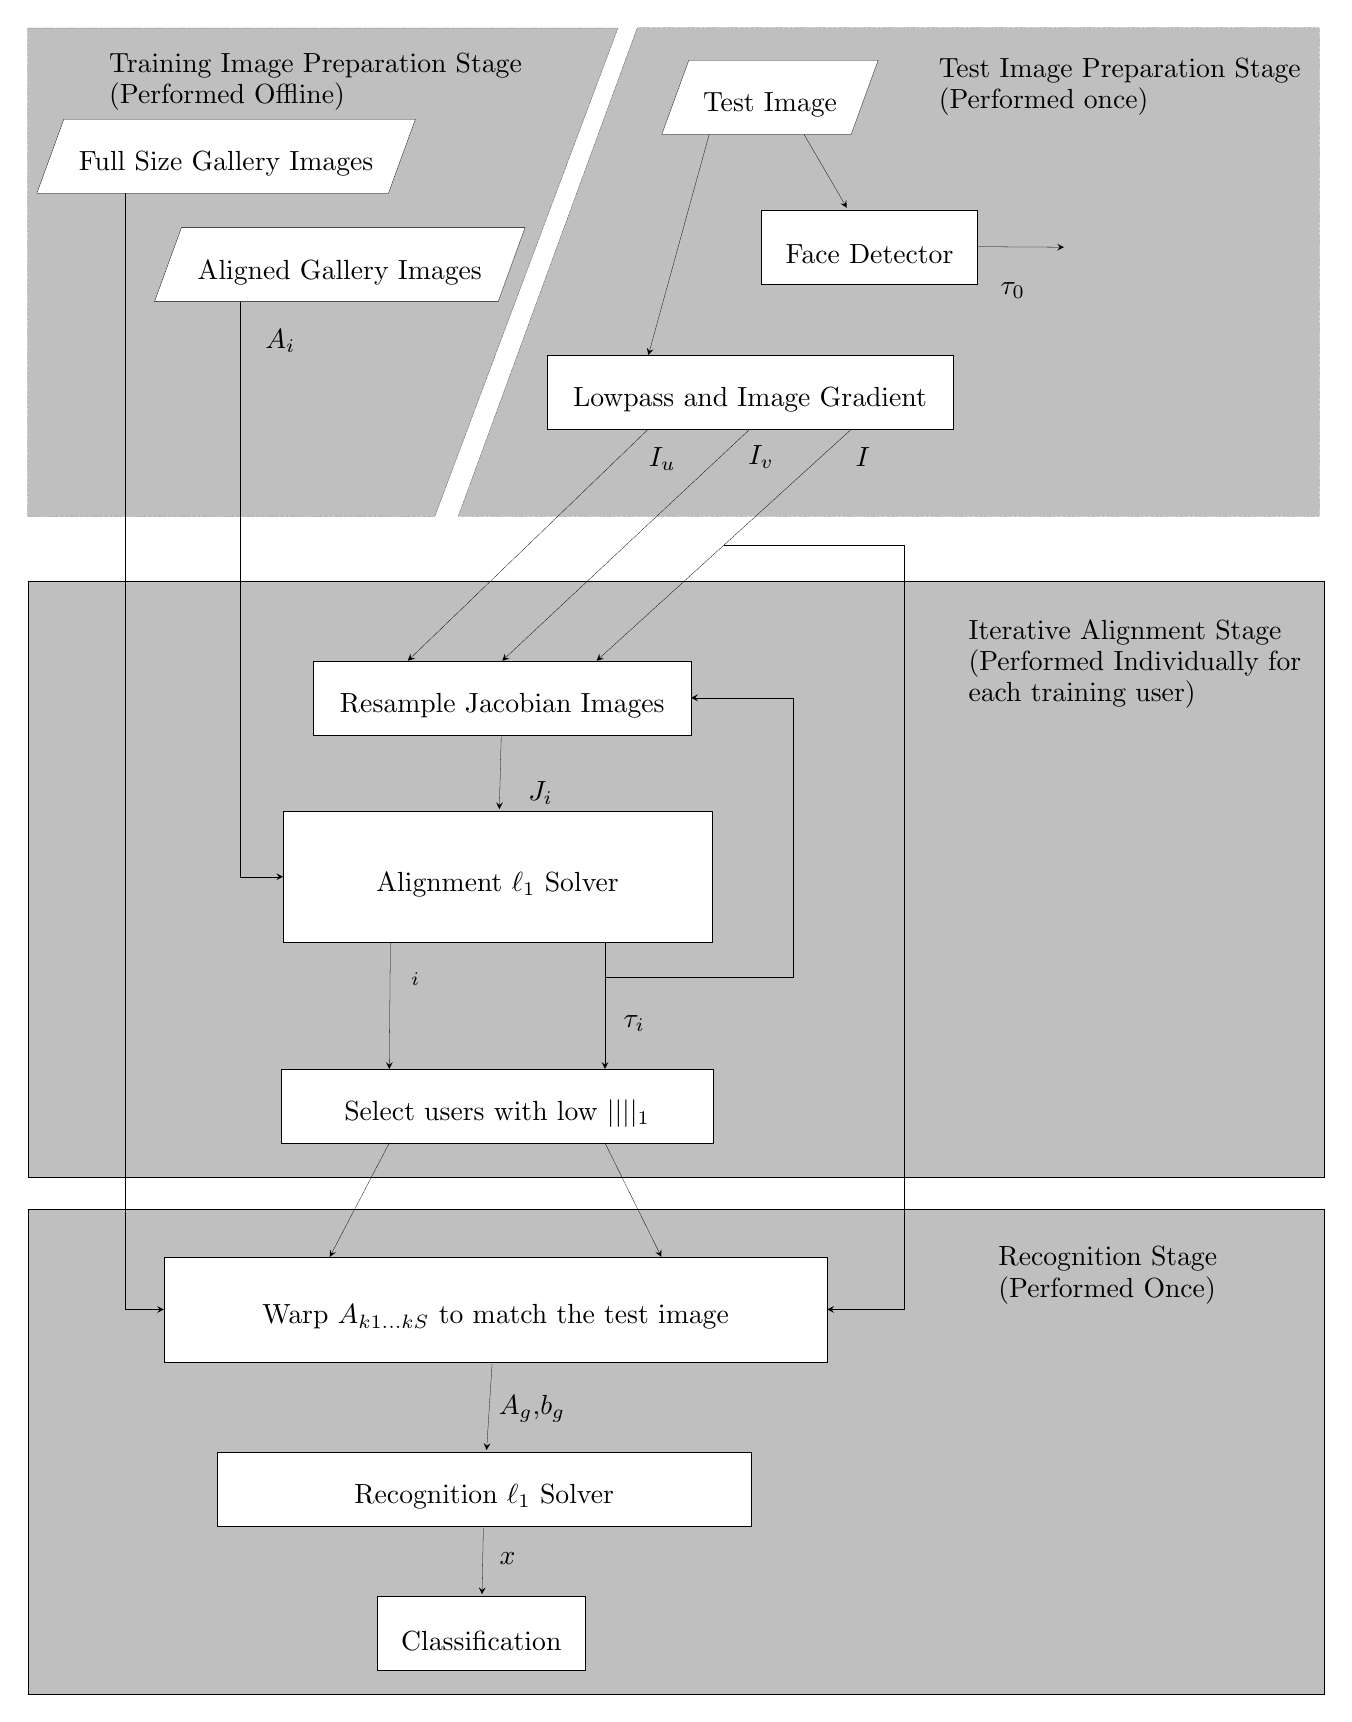
\begin{tikzpicture}
\pgftransformxscale{0.494667}
\pgftransformyscale{-0.494667}
\definecolor{dialinecolor}{rgb}{0.000000, 0.000000, 0.000000}
\pgfsetstrokecolor{dialinecolor}
\definecolor{dialinecolor}{rgb}{1.000000, 1.000000, 1.000000}
\pgfsetfillcolor{dialinecolor}
% setfont left to latex
\definecolor{dialinecolor}{rgb}{0.000000, 0.000000, 0.000000}
\pgfsetstrokecolor{dialinecolor}
\node[anchor=west] at (24.925000\du,42.952500\du){};
% setfont left to latex
\definecolor{dialinecolor}{rgb}{0.000000, 0.000000, 0.000000}
\pgfsetstrokecolor{dialinecolor}
\node[anchor=west] at (24.925000\du,42.952500\du){};
% setfont left to latex
\definecolor{dialinecolor}{rgb}{0.000000, 0.000000, 0.000000}
\pgfsetstrokecolor{dialinecolor}
\node[anchor=west] at (24.925000\du,42.952500\du){};
\definecolor{dialinecolor}{rgb}{0.749020, 0.749020, 0.749020}
\pgfsetfillcolor{dialinecolor}
\fill (6.494040\du,27.943300\du)--(6.494040\du,43.255071\du)--(39.770015\du,43.255071\du)--(39.770015\du,27.943300\du)--cycle;
\pgfsetlinewidth{0.100000\du}
\pgfsetdash{{\pgflinewidth}{0.200000\du}}{0cm}
\pgfsetdash{{\pgflinewidth}{0.200000\du}}{0cm}
\pgfsetmiterjoin
\definecolor{dialinecolor}{rgb}{0.000000, 0.000000, 0.000000}
\pgfsetstrokecolor{dialinecolor}
\draw (6.494040\du,27.943300\du)--(6.494040\du,43.255071\du)--(39.770015\du,43.255071\du)--(39.770015\du,27.943300\du)--cycle;
% setfont left to latex
\definecolor{dialinecolor}{rgb}{0.000000, 0.000000, 0.000000}
\pgfsetstrokecolor{dialinecolor}
\node at (23.132027\du,35.794186\du){};
\definecolor{dialinecolor}{rgb}{0.749020, 0.749020, 0.749020}
\pgfsetfillcolor{dialinecolor}
\fill (6.494040\du,44.061200\du)--(6.494040\du,56.519596\du)--(39.770015\du,56.519596\du)--(39.770015\du,44.061200\du)--cycle;
\pgfsetlinewidth{0.100000\du}
\pgfsetdash{{\pgflinewidth}{0.200000\du}}{0cm}
\pgfsetdash{{\pgflinewidth}{0.200000\du}}{0cm}
\pgfsetmiterjoin
\definecolor{dialinecolor}{rgb}{0.000000, 0.000000, 0.000000}
\pgfsetstrokecolor{dialinecolor}
\draw (6.494040\du,44.061200\du)--(6.494040\du,56.519596\du)--(39.770015\du,56.519596\du)--(39.770015\du,44.061200\du)--cycle;
% setfont left to latex
\definecolor{dialinecolor}{rgb}{0.000000, 0.000000, 0.000000}
\pgfsetstrokecolor{dialinecolor}
\node at (23.132027\du,50.485398\du){};
% setfont left to latex
\definecolor{dialinecolor}{rgb}{0.000000, 0.000000, 0.000000}
\pgfsetstrokecolor{dialinecolor}
\node[anchor=west] at (23.132000\du,35.599200\du){};
% setfont left to latex
\definecolor{dialinecolor}{rgb}{0.000000, 0.000000, 0.000000}
\pgfsetstrokecolor{dialinecolor}
\node[anchor=west] at (23.132000\du,35.599200\du){};
% setfont left to latex
\definecolor{dialinecolor}{rgb}{0.000000, 0.000000, 0.000000}
\pgfsetstrokecolor{dialinecolor}
\node[anchor=west] at (30.406100\du,29.259100\du){Iterative Alignment Stage};
% setfont left to latex
\definecolor{dialinecolor}{rgb}{0.000000, 0.000000, 0.000000}
\pgfsetstrokecolor{dialinecolor}
\node[anchor=west] at (30.406100\du,30.059100\du){(Performed Individually for};
% setfont left to latex
\definecolor{dialinecolor}{rgb}{0.000000, 0.000000, 0.000000}
\pgfsetstrokecolor{dialinecolor}
\node[anchor=west] at (30.406100\du,30.859100\du){each training user)};
% setfont left to latex
\definecolor{dialinecolor}{rgb}{0.000000, 0.000000, 0.000000}
\pgfsetstrokecolor{dialinecolor}
\node[anchor=west] at (31.173700\du,45.350700\du){Recognition Stage};
% setfont left to latex
\definecolor{dialinecolor}{rgb}{0.000000, 0.000000, 0.000000}
\pgfsetstrokecolor{dialinecolor}
\node[anchor=west] at (31.173700\du,46.150700\du){(Performed Once)};
\pgfsetlinewidth{0.100000\du}
\pgfsetdash{{\pgflinewidth}{0.200000\du}}{0cm}
\pgfsetdash{{\pgflinewidth}{0.200000\du}}{0cm}
\pgfsetmiterjoin
\pgfsetbuttcap
\definecolor{dialinecolor}{rgb}{0.749020, 0.749020, 0.749020}
\pgfsetfillcolor{dialinecolor}
\fill (6.494040\du,13.746400\du)--(21.645100\du,13.746400\du)--(16.943000\du,26.285100\du)--(6.494040\du,26.285100\du)--cycle;
\definecolor{dialinecolor}{rgb}{0.000000, 0.000000, 0.000000}
\pgfsetstrokecolor{dialinecolor}
\draw (6.494040\du,13.746400\du)--(21.645100\du,13.746400\du)--(16.943000\du,26.285100\du)--(6.494040\du,26.285100\du)--cycle;
% setfont left to latex
\definecolor{dialinecolor}{rgb}{0.000000, 0.000000, 0.000000}
\pgfsetstrokecolor{dialinecolor}
\node[anchor=west] at (8.342710\du,14.710900\du){Training Image Preparation Stage};
% setfont left to latex
\definecolor{dialinecolor}{rgb}{0.000000, 0.000000, 0.000000}
\pgfsetstrokecolor{dialinecolor}
\node[anchor=west] at (8.342710\du,15.510900\du){(Performed Offline)};
\pgfsetlinewidth{0.100000\du}
\pgfsetdash{{\pgflinewidth}{0.200000\du}}{0cm}
\pgfsetdash{{\pgflinewidth}{0.200000\du}}{0cm}
\pgfsetmiterjoin
\pgfsetbuttcap
\definecolor{dialinecolor}{rgb}{0.749020, 0.749020, 0.749020}
\pgfsetfillcolor{dialinecolor}
\fill (22.141100\du,13.740100\du)--(39.649500\du,13.740100\du)--(39.649500\du,26.278900\du)--(17.545800\du,26.278900\du)--cycle;
\definecolor{dialinecolor}{rgb}{0.000000, 0.000000, 0.000000}
\pgfsetstrokecolor{dialinecolor}
\draw (22.141100\du,13.740100\du)--(39.649500\du,13.740100\du)--(39.649500\du,26.278900\du)--(17.545800\du,26.278900\du)--cycle;
% setfont left to latex
\definecolor{dialinecolor}{rgb}{0.000000, 0.000000, 0.000000}
\pgfsetstrokecolor{dialinecolor}
\node[anchor=west] at (29.642500\du,14.831400\du){Test Image Preparation Stage};
% setfont left to latex
\definecolor{dialinecolor}{rgb}{0.000000, 0.000000, 0.000000}
\pgfsetstrokecolor{dialinecolor}
\node[anchor=west] at (29.642500\du,15.631400\du){(Performed once)};
\definecolor{dialinecolor}{rgb}{1.000000, 1.000000, 1.000000}
\pgfsetfillcolor{dialinecolor}
\fill (23.464443\du,14.572100\du)--(28.325620\du,14.572100\du)--(27.634076\du,16.472100\du)--(22.772900\du,16.472100\du)--cycle;
\pgfsetlinewidth{0.100000\du}
\pgfsetdash{}{0pt}
\pgfsetdash{}{0pt}
\pgfsetmiterjoin
\definecolor{dialinecolor}{rgb}{0.000000, 0.000000, 0.000000}
\pgfsetstrokecolor{dialinecolor}
\draw (23.464443\du,14.572100\du)--(28.325620\du,14.572100\du)--(27.634076\du,16.472100\du)--(22.772900\du,16.472100\du)--cycle;
% setfont left to latex
\definecolor{dialinecolor}{rgb}{0.000000, 0.000000, 0.000000}
\pgfsetstrokecolor{dialinecolor}
\node at (25.549260\du,15.717100\du){Test Image};
\definecolor{dialinecolor}{rgb}{1.000000, 1.000000, 1.000000}
\pgfsetfillcolor{dialinecolor}
\fill (13.826900\du,29.990700\du)--(13.826900\du,31.890700\du)--(23.521900\du,31.890700\du)--(23.521900\du,29.990700\du)--cycle;
\pgfsetlinewidth{0.100000\du}
\pgfsetdash{}{0pt}
\pgfsetdash{}{0pt}
\pgfsetmiterjoin
\definecolor{dialinecolor}{rgb}{0.000000, 0.000000, 0.000000}
\pgfsetstrokecolor{dialinecolor}
\draw (13.826900\du,29.990700\du)--(13.826900\du,31.890700\du)--(23.521900\du,31.890700\du)--(23.521900\du,29.990700\du)--cycle;
% setfont left to latex
\definecolor{dialinecolor}{rgb}{0.000000, 0.000000, 0.000000}
\pgfsetstrokecolor{dialinecolor}
\node at (18.674400\du,31.135700\du){Resample Jacobian Images};
\definecolor{dialinecolor}{rgb}{1.000000, 1.000000, 1.000000}
\pgfsetfillcolor{dialinecolor}
\fill (13.050000\du,33.850000\du)--(13.050000\du,37.221200\du)--(24.058800\du,37.221200\du)--(24.058800\du,33.850000\du)--cycle;
\pgfsetlinewidth{0.100000\du}
\pgfsetdash{}{0pt}
\pgfsetdash{}{0pt}
\pgfsetmiterjoin
\definecolor{dialinecolor}{rgb}{0.000000, 0.000000, 0.000000}
\pgfsetstrokecolor{dialinecolor}
\draw (13.050000\du,33.850000\du)--(13.050000\du,37.221200\du)--(24.058800\du,37.221200\du)--(24.058800\du,33.850000\du)--cycle;
% setfont left to latex
\definecolor{dialinecolor}{rgb}{0.000000, 0.000000, 0.000000}
\pgfsetstrokecolor{dialinecolor}
\node at (18.554400\du,35.730600\du){Alignment $\ell_1$ Solver};
\pgfsetlinewidth{0.100000\du}
\pgfsetdash{}{0pt}
\pgfsetdash{}{0pt}
\pgfsetbuttcap
{
\definecolor{dialinecolor}{rgb}{0.000000, 0.000000, 0.000000}
\pgfsetfillcolor{dialinecolor}
% was here!!!
\pgfsetarrowsend{stealth}
\definecolor{dialinecolor}{rgb}{0.000000, 0.000000, 0.000000}
\pgfsetstrokecolor{dialinecolor}
\draw (18.648326\du,31.939104\du)--(18.599693\du,33.801294\du);
}
% setfont left to latex
\definecolor{dialinecolor}{rgb}{0.000000, 0.000000, 0.000000}
\pgfsetstrokecolor{dialinecolor}
\node[anchor=west] at (11.250000\du,34.890000\du){};
\definecolor{dialinecolor}{rgb}{1.000000, 1.000000, 1.000000}
\pgfsetfillcolor{dialinecolor}
\fill (19.817600\du,22.143000\du)--(19.817600\du,24.043000\du)--(30.250100\du,24.043000\du)--(30.250100\du,22.143000\du)--cycle;
\pgfsetlinewidth{0.100000\du}
\pgfsetdash{}{0pt}
\pgfsetdash{}{0pt}
\pgfsetmiterjoin
\definecolor{dialinecolor}{rgb}{0.000000, 0.000000, 0.000000}
\pgfsetstrokecolor{dialinecolor}
\draw (19.817600\du,22.143000\du)--(19.817600\du,24.043000\du)--(30.250100\du,24.043000\du)--(30.250100\du,22.143000\du)--cycle;
% setfont left to latex
\definecolor{dialinecolor}{rgb}{0.000000, 0.000000, 0.000000}
\pgfsetstrokecolor{dialinecolor}
\node at (25.033850\du,23.288000\du){Lowpass and Image Gradient};
\definecolor{dialinecolor}{rgb}{1.000000, 1.000000, 1.000000}
\pgfsetfillcolor{dialinecolor}
\fill (25.332900\du,18.409900\du)--(25.332900\du,20.309900\du)--(30.875400\du,20.309900\du)--(30.875400\du,18.409900\du)--cycle;
\pgfsetlinewidth{0.100000\du}
\pgfsetdash{}{0pt}
\pgfsetdash{}{0pt}
\pgfsetmiterjoin
\definecolor{dialinecolor}{rgb}{0.000000, 0.000000, 0.000000}
\pgfsetstrokecolor{dialinecolor}
\draw (25.332900\du,18.409900\du)--(25.332900\du,20.309900\du)--(30.875400\du,20.309900\du)--(30.875400\du,18.409900\du)--cycle;
% setfont left to latex
\definecolor{dialinecolor}{rgb}{0.000000, 0.000000, 0.000000}
\pgfsetstrokecolor{dialinecolor}
\node at (28.104150\du,19.554900\du){Face Detector};
\definecolor{dialinecolor}{rgb}{1.000000, 1.000000, 1.000000}
\pgfsetfillcolor{dialinecolor}
\fill (9.987950\du,45.295200\du)--(9.987950\du,47.995200\du)--(27.017950\du,47.995200\du)--(27.017950\du,45.295200\du)--cycle;
\pgfsetlinewidth{0.100000\du}
\pgfsetdash{}{0pt}
\pgfsetdash{}{0pt}
\pgfsetmiterjoin
\definecolor{dialinecolor}{rgb}{0.000000, 0.000000, 0.000000}
\pgfsetstrokecolor{dialinecolor}
\draw (9.987950\du,45.295200\du)--(9.987950\du,47.995200\du)--(27.017950\du,47.995200\du)--(27.017950\du,45.295200\du)--cycle;
% setfont left to latex
\definecolor{dialinecolor}{rgb}{0.000000, 0.000000, 0.000000}
\pgfsetstrokecolor{dialinecolor}
\node at (18.502950\du,46.840200\du){Warp $A_{k1 \ldots kS}$ to match the test image};
\definecolor{dialinecolor}{rgb}{1.000000, 1.000000, 1.000000}
\pgfsetfillcolor{dialinecolor}
\fill (15.470400\du,54.006500\du)--(15.470400\du,55.906500\du)--(20.802900\du,55.906500\du)--(20.802900\du,54.006500\du)--cycle;
\pgfsetlinewidth{0.100000\du}
\pgfsetdash{}{0pt}
\pgfsetdash{}{0pt}
\pgfsetmiterjoin
\definecolor{dialinecolor}{rgb}{0.000000, 0.000000, 0.000000}
\pgfsetstrokecolor{dialinecolor}
\draw (15.470400\du,54.006500\du)--(15.470400\du,55.906500\du)--(20.802900\du,55.906500\du)--(20.802900\du,54.006500\du)--cycle;
% setfont left to latex
\definecolor{dialinecolor}{rgb}{0.000000, 0.000000, 0.000000}
\pgfsetstrokecolor{dialinecolor}
\node at (18.136650\du,55.151500\du){Classification};
% setfont left to latex
\definecolor{dialinecolor}{rgb}{0.000000, 0.000000, 0.000000}
\pgfsetstrokecolor{dialinecolor}
\node[anchor=west] at (28.104200\du,19.359900\du){};
\pgfsetlinewidth{0.100000\du}
\pgfsetdash{}{0pt}
\pgfsetdash{}{0pt}
\pgfsetbuttcap
{
\definecolor{dialinecolor}{rgb}{0.000000, 0.000000, 0.000000}
\pgfsetfillcolor{dialinecolor}
% was here!!!
\pgfsetarrowsend{stealth}
\definecolor{dialinecolor}{rgb}{0.000000, 0.000000, 0.000000}
\pgfsetstrokecolor{dialinecolor}
\draw (25.033800\du,24.043000\du)--(18.674400\du,29.990700\du);
}
\pgfsetlinewidth{0.100000\du}
\pgfsetdash{}{0pt}
\pgfsetdash{}{0pt}
\pgfsetbuttcap
{
\definecolor{dialinecolor}{rgb}{0.000000, 0.000000, 0.000000}
\pgfsetfillcolor{dialinecolor}
% was here!!!
\pgfsetarrowsend{stealth}
\definecolor{dialinecolor}{rgb}{0.000000, 0.000000, 0.000000}
\pgfsetstrokecolor{dialinecolor}
\draw (22.425700\du,24.043000\du)--(16.250600\du,29.990700\du);
}
\pgfsetlinewidth{0.100000\du}
\pgfsetdash{}{0pt}
\pgfsetdash{}{0pt}
\pgfsetbuttcap
{
\definecolor{dialinecolor}{rgb}{0.000000, 0.000000, 0.000000}
\pgfsetfillcolor{dialinecolor}
% was here!!!
\pgfsetarrowsend{stealth}
\definecolor{dialinecolor}{rgb}{0.000000, 0.000000, 0.000000}
\pgfsetstrokecolor{dialinecolor}
\draw (27.641900\du,24.043000\du)--(21.098100\du,29.990700\du);
}
% setfont left to latex
\definecolor{dialinecolor}{rgb}{0.000000, 0.000000, 0.000000}
\pgfsetstrokecolor{dialinecolor}
\node[anchor=west] at (27.506000\du,24.761200\du){$I$};
% setfont left to latex
\definecolor{dialinecolor}{rgb}{0.000000, 0.000000, 0.000000}
\pgfsetstrokecolor{dialinecolor}
\node[anchor=west] at (22.199300\du,24.802400\du){$I_u$};
\pgfsetlinewidth{0.100000\du}
\pgfsetdash{}{0pt}
\pgfsetdash{}{0pt}
\pgfsetbuttcap
{
\definecolor{dialinecolor}{rgb}{0.000000, 0.000000, 0.000000}
\pgfsetfillcolor{dialinecolor}
% was here!!!
\pgfsetarrowsend{stealth}
\definecolor{dialinecolor}{rgb}{0.000000, 0.000000, 0.000000}
\pgfsetstrokecolor{dialinecolor}
\draw (23.988200\du,16.472100\du)--(22.425700\du,22.143000\du);
}
\pgfsetlinewidth{0.100000\du}
\pgfsetdash{}{0pt}
\pgfsetdash{}{0pt}
\pgfsetbuttcap
{
\definecolor{dialinecolor}{rgb}{0.000000, 0.000000, 0.000000}
\pgfsetfillcolor{dialinecolor}
% was here!!!
\pgfsetarrowsend{stealth}
\definecolor{dialinecolor}{rgb}{0.000000, 0.000000, 0.000000}
\pgfsetstrokecolor{dialinecolor}
\draw (26.418800\du,16.472100\du)--(27.520491\du,18.359816\du);
}
% setfont left to latex
\definecolor{dialinecolor}{rgb}{0.000000, 0.000000, 0.000000}
\pgfsetstrokecolor{dialinecolor}
\node[anchor=west] at (28.248200\du,27.724100\du){};
% setfont left to latex
\definecolor{dialinecolor}{rgb}{0.000000, 0.000000, 0.000000}
\pgfsetstrokecolor{dialinecolor}
\node[anchor=west] at (31.230200\du,20.488200\du){$\tau_0$};
\definecolor{dialinecolor}{rgb}{1.000000, 1.000000, 1.000000}
\pgfsetfillcolor{dialinecolor}
\fill (7.418823\du,16.086600\du)--(16.445000\du,16.086600\du)--(15.753456\du,17.986600\du)--(6.727280\du,17.986600\du)--cycle;
\pgfsetlinewidth{0.100000\du}
\pgfsetdash{}{0pt}
\pgfsetdash{}{0pt}
\pgfsetmiterjoin
\definecolor{dialinecolor}{rgb}{0.000000, 0.000000, 0.000000}
\pgfsetstrokecolor{dialinecolor}
\draw (7.418823\du,16.086600\du)--(16.445000\du,16.086600\du)--(15.753456\du,17.986600\du)--(6.727280\du,17.986600\du)--cycle;
% setfont left to latex
\definecolor{dialinecolor}{rgb}{0.000000, 0.000000, 0.000000}
\pgfsetstrokecolor{dialinecolor}
\node at (11.586140\du,17.231600\du){Full Size Gallery Images};
\pgfsetlinewidth{0.100000\du}
\pgfsetdash{}{0pt}
\pgfsetdash{}{0pt}
\pgfsetmiterjoin
\pgfsetbuttcap
{
\definecolor{dialinecolor}{rgb}{0.000000, 0.000000, 0.000000}
\pgfsetfillcolor{dialinecolor}
% was here!!!
\pgfsetarrowsend{stealth}
{\pgfsetcornersarced{\pgfpoint{0.000000\du}{0.000000\du}}\definecolor{dialinecolor}{rgb}{0.000000, 0.000000, 0.000000}
\pgfsetstrokecolor{dialinecolor}
\draw (11.952169\du,20.770000\du)--(11.952169\du,35.535600\du)--(13.050000\du,35.535600\du);
}}
\pgfsetlinewidth{0.100000\du}
\pgfsetdash{}{0pt}
\pgfsetdash{}{0pt}
\pgfsetbuttcap
{
\definecolor{dialinecolor}{rgb}{0.000000, 0.000000, 0.000000}
\pgfsetfillcolor{dialinecolor}
% was here!!!
\pgfsetarrowsend{stealth}
\definecolor{dialinecolor}{rgb}{0.000000, 0.000000, 0.000000}
\pgfsetstrokecolor{dialinecolor}
\draw (30.875400\du,19.359900\du)--(33.098700\du,19.372700\du);
}
\definecolor{dialinecolor}{rgb}{1.000000, 1.000000, 1.000000}
\pgfsetfillcolor{dialinecolor}
\fill (11.356800\du,50.303600\du)--(11.356800\du,52.203600\du)--(25.061036\du,52.203600\du)--(25.061036\du,50.303600\du)--cycle;
\pgfsetlinewidth{0.100000\du}
\pgfsetdash{}{0pt}
\pgfsetdash{}{0pt}
\pgfsetmiterjoin
\definecolor{dialinecolor}{rgb}{0.000000, 0.000000, 0.000000}
\pgfsetstrokecolor{dialinecolor}
\draw (11.356800\du,50.303600\du)--(11.356800\du,52.203600\du)--(25.061036\du,52.203600\du)--(25.061036\du,50.303600\du)--cycle;
% setfont left to latex
\definecolor{dialinecolor}{rgb}{0.000000, 0.000000, 0.000000}
\pgfsetstrokecolor{dialinecolor}
\node at (18.208918\du,51.448600\du){Recognition $\ell_1$ Solver};
\pgfsetlinewidth{0.100000\du}
\pgfsetdash{}{0pt}
\pgfsetdash{}{0pt}
\pgfsetmiterjoin
\pgfsetbuttcap
{
\definecolor{dialinecolor}{rgb}{0.000000, 0.000000, 0.000000}
\pgfsetfillcolor{dialinecolor}
% was here!!!
\pgfsetarrowsend{stealth}
{\pgfsetcornersarced{\pgfpoint{0.000000\du}{0.000000\du}}\definecolor{dialinecolor}{rgb}{0.000000, 0.000000, 0.000000}
\pgfsetstrokecolor{dialinecolor}
\draw (21.306600\du,37.221200\du)--(21.306600\du,38.050000\du)--(21.312500\du,38.050000\du)--(21.312500\du,40.470000\du);
}}
\pgfsetlinewidth{0.100000\du}
\pgfsetdash{}{0pt}
\pgfsetdash{}{0pt}
\pgfsetbuttcap
{
\definecolor{dialinecolor}{rgb}{0.000000, 0.000000, 0.000000}
\pgfsetfillcolor{dialinecolor}
% was here!!!
\pgfsetarrowsend{stealth}
\definecolor{dialinecolor}{rgb}{0.000000, 0.000000, 0.000000}
\pgfsetstrokecolor{dialinecolor}
\draw (15.802200\du,37.221200\du)--(15.775000\du,40.470000\du);
}
% setfont left to latex
\definecolor{dialinecolor}{rgb}{0.000000, 0.000000, 0.000000}
\pgfsetstrokecolor{dialinecolor}
\node[anchor=west] at (16.096600\du,38.150600\du){$\e_i$};
\pgfsetlinewidth{0.100000\du}
\pgfsetdash{}{0pt}
\pgfsetdash{}{0pt}
\pgfsetbuttcap
{
\definecolor{dialinecolor}{rgb}{0.000000, 0.000000, 0.000000}
\pgfsetfillcolor{dialinecolor}
% was here!!!
\pgfsetarrowsend{stealth}
\definecolor{dialinecolor}{rgb}{0.000000, 0.000000, 0.000000}
\pgfsetstrokecolor{dialinecolor}
\draw (18.189395\du,52.253907\du)--(18.156173\du,53.956193\du);
}
\pgfsetlinewidth{0.100000\du}
\pgfsetdash{}{0pt}
\pgfsetdash{}{0pt}
\pgfsetmiterjoin
\pgfsetbuttcap
{
\definecolor{dialinecolor}{rgb}{0.000000, 0.000000, 0.000000}
\pgfsetfillcolor{dialinecolor}
% was here!!!
\pgfsetarrowsend{stealth}
{\pgfsetcornersarced{\pgfpoint{0.000000\du}{0.000000\du}}\definecolor{dialinecolor}{rgb}{0.000000, 0.000000, 0.000000}
\pgfsetstrokecolor{dialinecolor}
\draw (24.370000\du,27.016800\du)--(28.999500\du,27.016800\du)--(28.999500\du,46.645200\du)--(27.018000\du,46.645200\du);
}}
\pgfsetlinewidth{0.100000\du}
\pgfsetdash{}{0pt}
\pgfsetdash{}{0pt}
\pgfsetbuttcap
{
\definecolor{dialinecolor}{rgb}{0.000000, 0.000000, 0.000000}
\pgfsetfillcolor{dialinecolor}
% was here!!!
\pgfsetarrowsend{stealth}
\definecolor{dialinecolor}{rgb}{0.000000, 0.000000, 0.000000}
\pgfsetstrokecolor{dialinecolor}
\draw (18.413613\du,48.045384\du)--(18.272699\du,50.253951\du);
}
% setfont left to latex
\definecolor{dialinecolor}{rgb}{0.000000, 0.000000, 0.000000}
\pgfsetstrokecolor{dialinecolor}
\node[anchor=west] at (18.367000\du,53.041300\du){$x$};
% setfont left to latex
\definecolor{dialinecolor}{rgb}{0.000000, 0.000000, 0.000000}
\pgfsetstrokecolor{dialinecolor}
\node[anchor=west] at (18.349600\du,49.203000\du){$A_g$,$b_g$};
% setfont left to latex
\definecolor{dialinecolor}{rgb}{0.000000, 0.000000, 0.000000}
\pgfsetstrokecolor{dialinecolor}
\node[anchor=west] at (24.755000\du,24.750000\du){$I_v$};
% setfont left to latex
\definecolor{dialinecolor}{rgb}{0.000000, 0.000000, 0.000000}
\pgfsetstrokecolor{dialinecolor}
\node[anchor=west] at (12.355000\du,21.787500\du){$A_i$};
% setfont left to latex
\definecolor{dialinecolor}{rgb}{0.000000, 0.000000, 0.000000}
\pgfsetstrokecolor{dialinecolor}
\node[anchor=west] at (19.105000\du,33.387500\du){$J_i$};
\definecolor{dialinecolor}{rgb}{1.000000, 1.000000, 1.000000}
\pgfsetfillcolor{dialinecolor}
\fill (10.437793\du,18.870000\du)--(19.261470\du,18.870000\du)--(18.569926\du,20.770000\du)--(9.746250\du,20.770000\du)--cycle;
\pgfsetlinewidth{0.100000\du}
\pgfsetdash{}{0pt}
\pgfsetdash{}{0pt}
\pgfsetmiterjoin
\definecolor{dialinecolor}{rgb}{0.000000, 0.000000, 0.000000}
\pgfsetstrokecolor{dialinecolor}
\draw (10.437793\du,18.870000\du)--(19.261470\du,18.870000\du)--(18.569926\du,20.770000\du)--(9.746250\du,20.770000\du)--cycle;
% setfont left to latex
\definecolor{dialinecolor}{rgb}{0.000000, 0.000000, 0.000000}
\pgfsetstrokecolor{dialinecolor}
\node at (14.503860\du,20.015000\du){Aligned Gallery Images};
\pgfsetlinewidth{0.100000\du}
\pgfsetdash{}{0pt}
\pgfsetdash{}{0pt}
\pgfsetmiterjoin
\pgfsetbuttcap
{
\definecolor{dialinecolor}{rgb}{0.000000, 0.000000, 0.000000}
\pgfsetfillcolor{dialinecolor}
% was here!!!
\pgfsetarrowsend{stealth}
{\pgfsetcornersarced{\pgfpoint{0.000000\du}{0.000000\du}}\definecolor{dialinecolor}{rgb}{0.000000, 0.000000, 0.000000}
\pgfsetstrokecolor{dialinecolor}
\draw (8.983824\du,17.986600\du)--(8.983824\du,46.645200\du)--(9.987950\du,46.645200\du);
}}
\pgfsetlinewidth{0.100000\du}
\pgfsetdash{}{0pt}
\pgfsetdash{}{0pt}
\pgfsetmiterjoin
\pgfsetbuttcap
{
\definecolor{dialinecolor}{rgb}{0.000000, 0.000000, 0.000000}
\pgfsetfillcolor{dialinecolor}
% was here!!!
\pgfsetarrowsend{stealth}
{\pgfsetcornersarced{\pgfpoint{0.000000\du}{0.000000\du}}\definecolor{dialinecolor}{rgb}{0.000000, 0.000000, 0.000000}
\pgfsetstrokecolor{dialinecolor}
\draw (21.300000\du,38.100000\du)--(26.150000\du,38.100000\du)--(26.150000\du,30.940700\du)--(23.521900\du,30.940700\du);
}}
% setfont left to latex
\definecolor{dialinecolor}{rgb}{0.000000, 0.000000, 0.000000}
\pgfsetstrokecolor{dialinecolor}
\node[anchor=west] at (21.550000\du,39.300000\du){$\tau_i$};
\definecolor{dialinecolor}{rgb}{1.000000, 1.000000, 1.000000}
\pgfsetfillcolor{dialinecolor}
\fill (13.006200\du,40.470000\du)--(13.006200\du,42.370000\du)--(24.081200\du,42.370000\du)--(24.081200\du,40.470000\du)--cycle;
\pgfsetlinewidth{0.100000\du}
\pgfsetdash{}{0pt}
\pgfsetdash{}{0pt}
\pgfsetmiterjoin
\definecolor{dialinecolor}{rgb}{0.000000, 0.000000, 0.000000}
\pgfsetstrokecolor{dialinecolor}
\draw (13.006200\du,40.470000\du)--(13.006200\du,42.370000\du)--(24.081200\du,42.370000\du)--(24.081200\du,40.470000\du)--cycle;
% setfont left to latex
\definecolor{dialinecolor}{rgb}{0.000000, 0.000000, 0.000000}
\pgfsetstrokecolor{dialinecolor}
\node at (18.543700\du,41.615000\du){Select users with low $||\e||_1$};
\pgfsetlinewidth{0.100000\du}
\pgfsetdash{}{0pt}
\pgfsetdash{}{0pt}
\pgfsetbuttcap
{
\definecolor{dialinecolor}{rgb}{0.000000, 0.000000, 0.000000}
\pgfsetfillcolor{dialinecolor}
% was here!!!
\pgfsetarrowsend{stealth}
\definecolor{dialinecolor}{rgb}{0.000000, 0.000000, 0.000000}
\pgfsetstrokecolor{dialinecolor}
\draw (15.775000\du,42.370000\du)--(14.245500\du,45.295200\du);
}
\pgfsetlinewidth{0.100000\du}
\pgfsetdash{}{0pt}
\pgfsetdash{}{0pt}
\pgfsetbuttcap
{
\definecolor{dialinecolor}{rgb}{0.000000, 0.000000, 0.000000}
\pgfsetfillcolor{dialinecolor}
% was here!!!
\pgfsetarrowsend{stealth}
\definecolor{dialinecolor}{rgb}{0.000000, 0.000000, 0.000000}
\pgfsetstrokecolor{dialinecolor}
\draw (21.312500\du,42.370000\du)--(22.760500\du,45.295200\du);
}
\end{tikzpicture}
}
\includegraphics[scale=1.4]{figures_ijcb/pipeline_simplified.pdf}
\caption{The face recognition pipeline.  }
\label{fig:pipeline}
\end{figure}

\section{Hardware Concurrency} \label{sec:concurrency}
In this section we discuss the levels of concurrency available in the hardware
architectures considered in this thesis, as well as other aspects of the
hardware that are important for performance.  In particular, since caches
(regions of on-chip memory) are often orders of magnitude faster than off-chip
memory, their sizes and speeds have a dramatic effect on performance.  We give a
brief overview of the caches that are available in our target architectures,
and defer discussion of their performance effects to Sections
\ref{sec:alignment_implementation_cpu} and
\ref{sec:alignment_implementation_gpu}.

Our discussion and experiments will address the most common hardware
configuration for engineering workstations: a motherboard with two quad-core
processors and a PCIe card with a single high-end GPU.  
Recognition involving more than a few hundred subjects with contemporary hardware
would require a server (or cluster) configuration with an expandable 
number of processors.  We will not address efficient parallelization for 
these systems, which may have additional challenges associated with
their non-shared memory model.
%\footnote{Non-shared memory configurations include CPU blade servers, multi-GPU servers, and clusters}.
Unless otherwise specified, all implementations utilize single precision
floating point datatypes.  

\subsection{CPU Hardware Concurrency}
\label{sec:CPU-concurrency}
The main defining characteristics of contemporary multi-core CPU architectures
are that they have two levels of concurrency, relatively large amounts of
cache, and relatively high clock speeds. The baseline architecture for our experiments 
is a Linux workstation with two
quad-core Intel Nehalem E5530 processors clocked at 2.4 GHz.  Each processor
has its own memory interface, and is directly interfaced to half of the RAM
installed in the machine.  The amount of RAM exceeds the amount used
by the algorithms, and is not an important performance consideration.  

\begin{figure}
\centering
\subfigure[The larger algorithm data structures]
{
	\includegraphics[scale=1.7]{figures_ijcb/arrays.pdf}
	\label{fig:arrays}
}
\subfigure[The caches on a E5530 CPU]
{
	\includegraphics[scale=1.7]{figures_ijcb/cpu_caches.pdf}
	\label{fig:cpu_caches}
}
\subfigure[The caches on a GTX480 GPU]
{
	\includegraphics[scale=1.7]{figures_ijcb/gpu_caches.pdf}
	\label{fig:gpu_caches}
}
\label{fig:caches}
\caption{A visual comparison of the algorithm working set to the CPU and GPU
caches.  Note: Although the aspect ratio could not be preserved, all arrays and
caches are drawn so that the area is proportional to the size of the data. } 
\end{figure}

% CPU CACHE DISCUSSION
%2MB = 2**21 bytes
%64*64*4 = 2**14 bytes = 16384 bytes per image
%... so can fit 2**7  = 128 images.
Each core has a private 32\,KiB L1 data cache and a private 256\,KiB L2 cache.
%16MB = 2**24 bytes = 16777216 bytes
%64*64*4 = 2**14 bytes = 16384 bytes per image
%... so can fit 2**10  = 1024 images.
Each processor further has 8\,MiB of L3 cache that is shared by the four cores.
Overall, the algorithm has approximately 16\,MiB of L3 cache
available for a dual-processor configuration.  

For floating-point instructions, each core also has a vector processing unit
(SSE) capable of performing the same arithmetic operation on four single-precision 
floating point values simultaneously.
There are thus two important levels of concurrency that need to be exploited to
efficiently use a modern CPU: {\em core-level} concurrency and {\em SSE-level}
concurrency. 

\subsection{GPU Hardware Concurrency} 
The main defining characteristics of contemporary multi-core GPU architectures
are that they have two (much wider) levels of concurrency, relatively small amounts of
 cache, and relatively low clock speeds.  Whereas most of the transistors on
a typical CPU are dedicated either to cache or to hardware that enables higher
clock speeds (such as branch prediction, out-of-order instruction execution, etc.),
most of the transistors on a GPU are dedicated to arithmetic logic units.
For our GPU implementations, we target NVIDIA Fermi GPU architecture (\eg the GTX 480
GPU addressed in this chapter).  An explanation of the GPU programming model (CUDA) at a useful level of completeness would take more space than is available here, so we will instead frame our discussion in terms of 
hardware capabilities. 
%\footnote{A discussion of the CUDA programming model can be found in the NVIDIA C for CUDA Programming Guide}
CUDA programmable GPUs are comprised of several
\emph{streaming multiprocessors} (SM), each of which is roughly analogous to a CPU core.
For Fermi architecture GPUs there are up to 16 SMs, and each SM is capable of executing up to 64 single precision 
floating point operations
concurrently.\footnote{In CUDA terms, the warp width is 32, and the floating pipeline can
issue up to two warps simultaneously.}

% GPU CACHE DISCUSSION
% for L2 cache
% 768KB = 786432 bytes
% 64*64*4 = 2**14 bytes = 16384 bytes per image
% 48 images
Each SM contains its own L1-cache, which is divided between hardware managed
and software managed (``shared") memory.  Additionally, all SMs share a common
L2-cache.  For our system, each SM has 64 KiB of L1 cache, and all SMs share
768KB of L2 cache. 
%The cache hierarchy 
The relatively small amount
of cache (1/23 as much as CPU L3) on the GPU is balanced by a significantly
higher bandwidth between the processor chip and off-chip memory (DRAM) compared
to the CPU.  A scale drawing of the caches available on the GPU can be seen in Figure \ref{fig:gpu_caches}.
The GPU has its own memory system, and any data the GPU uses must first be
transferred from CPU DRAM to GPU DRAM over PCIe.  For our application,
this transfer overhead can be amortized over a large amount of computation and is
not a major concern.

While the programming model for
the SIMD units of each SM is somewhat more flexible than on the CPU,
leveraging the flexibility typically comes at the cost of reduced concurrency.\footnote{
In CUDA terms, code branches that cause warp divergence usually
result in serialization of the different groups of threads}  Therefore, for
the purposes of comparing hardware architectures, the SIMD units on the GPU are
roughly analogous to the CPU SIMD units. Thus, in summary, the GPU hardware 
provides two levels of concurrency: {\em SM-level}
concurrency and {\em thread-level} concurrency.  Note that the GPU provides more
concurrency than a CPU at both levels (14 SMs vs. 8 cores) and (64 wide vs. 4 wide SIMD
units).


\section{Parallelism in the Face Alignment Stage}
\label{sec:alignment}

We will next discuss the parallelism available in the face recognition
pipeline, and propose techniques for exploiting this parallelism on the GPU and CPU hardware 
described in the previous section.  In this section we first focus on the
face alignment stage (see Figure \ref{fig:pipeline}).

Face alignment \eqref{eq:l1min_alignment} estimates an image transformation
$\tau$ that rectifies the query image $\tilde{\bb}$ with possible pose
variation w.r.t. each training class $A_i$, which leads to the minimal sparsity
in error $\e$ after the alignment. Note that directly solving
\eqref{eq:l1min_alignment} is inefficient since it is a non-convex problem
and may exhibit local minima.
However, given a good initial estimate of the
transformation $\tau$ (\eg provided by an accurate face detector), the optimal
solution for $\tau$ can be sought iteratively by linearization at each $j$th
step:
\begin{equation}
\min_{\x, \e, \Delta \tau_j}\|\e\|_1\quad \subj\quad \tilde\bb\circ\tau_j +  J_j\Delta \tau_j = A_i\x + \e,
\end{equation}
where $J_j = \nabla_{\tau_j}(\tilde\bb\circ\tau_j)$ is the Jacobian, and
$\Delta \tau$ is a step update to $\tau$. Denote $\bb_j =
\tilde\bb\circ\tau_j$, $B_j = [A_i, -J_j]$ and $\ww^T = [\x^T, \Delta
\tau^T]$; then the update $\Delta \tau$ can be computed by solving the
following linear program:
\begin{equation}
\min_{\ww, \e}\|\e\|_1\quad \subj\quad \bb_j = B_j\ww + \e.
\label{eq:alignment-linearization}
\end{equation}
%If the warping $\tau$ is constrained to be a similarity transform,
%it can be paramaterized in such a way that the computation of $\frac{\partial \bb}{\partial \tau_p}$
%reduces to several linear vector operations involving pixel coordinates $(u,v)$, $\tau \in \Re^4$,
%and the image gradients $\f_x, \f_y \in \Re^M$, the latter of which only has to be computed
%once per test image.  
The per-class alignment algorithm via ALM is summarized in Algorithm
\ref{alg:iterative_alignment}. 
%In terms of computational complexity, one significant
%term is the computation of the matrix pseudo-inverse $B_j^\dagger$, whose
%computational cost is bounded by $O(n_i^2m + n_i^3)$. However, for per-class face
%alignment, since both $B_j$ and $J_{j}$ are very tall matrices (\ie $m\gg n_i$
%for all $i=1, \cdots, K$ classes), we find that the computation cost is still
%dominated by the frequently computed matrix-vector multiplications in the
%inner loop.
\begin{algorithm}[ht!]
\caption{\bf (Face Alignment via ALM)} \label{alg:iterative_alignment}
\small
{\bf Input:} $\bb$, $A_i$, $\x_0 = \mathbf{0}$, $\tau_0$, and $J_0$.
\begin{algorithmic}[1]
\WHILE{not converged ($j = 1,2,\ldots$)}
\STATE Update $\bb_j \leftarrow \frac{\bb\circ \tau_{j-1}}{\|\bb\circ \tau_{j-1}\|}$; $B_j= [A_i, -J_{j-1}]$ and corresponding $(B_j^\dagger)^T$
\STATE Initialize $\ww_0 = \mathbf 0$, $\blambda_0 = \mathbf 0$
\WHILE{not converged ($k = 1,2,\ldots$)}
\STATE $\uu_0\leftarrow \ww_{k-1}$; $\zz_0\leftarrow \e_{k-1}$
\WHILE{not converged ($l = 1,2,\ldots$)}
\STATE $\zz_l \leftarrow \shrink\left(\bb_j - B_j\uu_{l-1} + \frac{\blambda_{k}}{\mu_{k-1}}, \frac{1}{\mu_{k-1}}\right)$
\STATE $\uu_l \leftarrow B_j^\dagger \left(\bb_j - \zz_{l} + \frac{\blambda_{k-1}}{\mu_{k-1}} \right) $
\ENDWHILE
\STATE $\ww_k \leftarrow \uu_l$; $\e_k \leftarrow \zz_l$
\STATE $\blambda_{k} \leftarrow \blambda_{k-1} + \mu_{k-1} (\bb_j - B_j\ww_{k} - \e_{k})$
\STATE $\mu_{k} \leftarrow \rho\mu_{k-1}$
\ENDWHILE
\STATE Update $\e_j$, $\tau_j$, and $J_j$
\ENDWHILE
\end{algorithmic}
{\bf Output:} $\tau_i^*\leftarrow \tau_j, \e_i^*\leftarrow \e_j$
\end{algorithm}

In summary, the alignment stage essentially contains two levels of available
parallelism. At the higher level, there are per-class alignment problems
that are solved independently, or \emph{problem-level parallelism}.  At a lower
level, the first-order linear algebraic operations exhibit parallelism within
image operations, \ie at the pixel level.  We call this \emph{pixel-level
parallelism}.  The following two sections discuss methods for exploiting
these two levels of parallelism on CPU and GPU architectures.

\subsection{CPU Implementation} 
\label{sec:alignment_implementation_cpu}

Optimal implementation of Algorithm \ref{alg:iterative_alignment} on a multi-core CPU must take 
into account the properties of the cache hierarchy. In general, cache that is 
closer to the core (i.e. L1 cache) has higher bandwidth but smaller size compared to cache
that is farther from the core (L3 cache).  For reference, Figure \ref{fig:cpu_caches} 
shows the the sizes of L2 and L3 caches of the Intel E5530 CPU, 
which is a representative example of a modern multi-core CPU. 

For the E5530, the L2 cache in each core is only able to store about 16 images.
For the image alignment problem, the number of training images per class is
typically larger than 16.  
In this chapter, we compare two mappings of the parallelism available in the alignment
stage to the concurrency available on the CPU: a naive implementation that is purely 
based on stock libraries and compilers, and a manually optimized version we advocate.

The naive implementation disregards 
problem-level parallelism, and instead maps pixel-level parallelism
onto both the core-level and the SSE-level concurrency provided by the CPU.  In
other words, alignment of the query image is performed
against a single subject at a time using all available cores on
the processors.  The potential advantage of this implementation is that all of the variables
for the inner loop, most notably $B_j$ and $B_j^\dagger$, fit in L2 cache.  

In contrast, our manually optimized implementation maps problem-level parallelism onto core-level
concurrency, and maps pixel-level parallelism onto SSE-level concurrency.  In
other words, eight instances of \eqref{eq:alignment-linearization} are executed
in parallel with each problem running on one of the eight cores.  The advantage
of this implementation is that since the cores are operating on different
alignment problem instances, no data is shared between cores, and therefore no
synchronization is necessary between the cores.  Furthermore, even with eight
problem instances running concurrently, the local variables for the inner
loop still fit in L3 cache.  Because of the sequential data access patterns of
the solver, the CPU hardware is able to use the full L3 cache bandwidth, which is 
high enough to make the program CPU limited, rather than memory limited.  
For these reasons, this implementation outperforms the previous naive solution.

%64 byte cache line-size per clock.  L3 cache running at lower clock than cpu.  Two reads and a write per clock.
%4 floats at a time in SSE.

In both implementations, most of the operations take
advantage of Intel Math Kernel Library (MKL), a commercial implementation of
the standard Basic Linear Algebra Subprograms (BLAS). For the image resampling
step, we make use of the Intel Integrated Performance Primitives (IPP) library.
Both MKL and IPP are optimized for Intel multi-core CPUs, and are able to
automatically utilize both core-level and vector-level concurrency (for the first implementation),
but are also available in single-threaded versions (for the second implementation). For 
operations that are not optimized by Intel in-house libraries, such as the soft thresholding
operator in step 7 of Algorithm \ref{alg:iterative_alignment}, we achieve 
vector-level concurrency via
the automatic vectorization facilities of the Intel C++ compiler (ICC) \cite{dulong1999overview}.
To achieve core-level concurrency we make use of the Open MP API. \cite{dagum2002openmp} 
%We shall compare the performance of the two parallelism methods in Section \ref{sec:experiment}.

\subsection{GPU Implementation} 
\label{sec:alignment_implementation_gpu}
While on the CPU, algorithm performance is highly dependent on effective
cache usage; cache is relatively unimportant on the GPU for ALM based
$\ell_1$-minimization.  As can be seen in Figure \ref{fig:gpu_caches}, the GPU has 
a very small amount of cache compared to the CPU.  While it might be possible
to fit a single instance of the alignment problem (with a slightly reduced problem size)
into L2 cache, this would not be an efficient use of the GPU's resources.
The strength of the GPU's memory architecture for our purposes is its ability to sustain a very
high bandwidth to DRAM.  This bandwidth is achieved by having a very large number of
threads issuing interleaved memory requests.  Solving many alignment problem instances
concurrently increases the number of threads that can be used.

Therefore, our recommended GPU implementation is strikingly similar in spirit
to our recommended CPU implementation: on the CPU we use the cores to solve
multiple instances concurrently, and on the GPU we use multiple SMs for the 
same purpose.\footnote{In CUDA terms, our proposed alignment stage
implementation consists of a single kernel that performs alignment for all
subject classes.  Each instance of the alignment problem is assigned its own
thread block, and the GPU hardware schedules as many thread blocks to run
concurrently as the hardware will allow.} The number of subject classes that
are actually scheduled to run concurrently is chosen by the GPU hardware, 
but can be indirectly influenced by manual tuning of the code (i.e., the kernel launch
configuration in CUDA terms). We have empirically determined
that performance is highest with 5-7 subject classes aligned simultaneously on each SM.
%This mapping of the problem-level parallelism onto the SM-level
%concurrency is illustrated in Figure \ref{fig:alignment_mapping_gpu}.
%\begin{figure}
%\centering
%\includegraphics[width=3.4in]{figures_ijcb/alignment_mapping_gpu}
%\caption{Proposed mapping of alignment parallelism onto GPU concurrency}
%\label{fig:alignment_mapping_gpu}
%\end{figure}

Several other aspects of the implementation merit discussion.  
First of all, we take advantage of the GPU's special hardware dedicated to bilinear interpolation
for the computation of $b(\tau)$ and $J(\tau)$, which essentially consist of resampled
versions of the test image and its derivatives.
Second, since there are no standard CUDA libraries that work at the SM level, we use a
custom routine for computing $B_j^\dagger = (B_j^TB_j)^{-1} B^T = G^{-1} B_j^T$, with $G$
inverted using Gaussian elimination with partial pivoting.  To achieve
precision comparable to the single precision LAPACK routines in Intel's MKL
with this simplistic algorithm, we use double precision.  Since $G$ is only $n
\times n$ and $B_j^\dagger$ is only computed once per optimization problem, the
cost of the inversion is dwarfed by the cost of other steps.  
Similarly, sums and dot-products of large vectors are also
performed in double precision.
%The lack of a atomic floating point addition on the GPU
%significantly reduces the perfomance of this step of the algorithm.
%In Section \ref{sec:experiment}, we show the performance of our CPU and GPU
%implementations running on synthetic and real image data.

\section{Parallelization of the Face Recognition Stage} 
\label{sec:recognition}
After the face alignment stage is complete, the 20 subject classes with lowest
alignment error are selected for recognition, $\bb$ and $A_i$ are re-sampled to a common alignment
using $\tau_i$, and $A_i$ are concatenated into a new matrix $A$.
A sparse representation of $\bb$ w.r.t $A$ is then recovered
by solving a single $\ell_1$-minimization problem, as shown
in \eqref{eq:l1min_denoise}, using Algorithm \ref{alg:alm_rec}.  The
coefficients in $\x$ are then used to compute error residuals that are used for
classification.  
%This recognition algorithm has
%been extensively studied in
%\cite{WrightJ2009-PAMI,YangA2010-ICIP,WagnerA2011-PAMI}.
In this stage of the algorithm, there is no problem-level
parallelism to exploit, so this section will discuss how to exploit pixel-level parallelism
on both CPU and GPU hardware.
Then in Section \ref{sec:experiment}, we will benchmark the
performance of the two architectures and further demonstrate the speed
gains achieved by our proposed implementations over previously published implementations.

\begin{algorithm}[t]
\caption{\bf (Face Recognition via ALM)} \label{alg:alm_rec} 
\begin{algorithmic}[1]
\begin{small}
\STATE {\bf Input:} $\bb \in \Re^m$, $A \in \Re^{m \times n}$,
$\x_1 = \mathbf{0}$, $\e_1 = \bb$, $\y_1 =
\mathbf{0}$.
\WHILE{not converged ($k = 1,2,\ldots$)}
\STATE $\e_{k+1} = \shrink(\bb - A\x_k +
\frac{1}{\mu}\y_k, \frac{1}{\mu})$;
\STATE $t_1\leftarrow 1$, $\z_1 \leftarrow \x_k$, $\w_1 \leftarrow \x_k$;
\WHILE{not converged ($l = 1,2,\ldots$)}
\STATE $\w_{l+1} \leftarrow \shrink(\z_l +
\frac{1}{\gamma}A^T(\bb - A\z_l - \e_{k+1} +
\frac{1}{\mu}\y_k), \frac{1}{\mu\gamma})$;
\STATE $t_{l+1} \leftarrow \frac{1}{2}( 1 +
\sqrt{1+4t_l^2})$;
\STATE $\z_{l+1} \leftarrow \w_{l+1} + \frac{t_l - 1}{t_{l+1}}(\w_{l+1} - \w_l)$;
\ENDWHILE
\STATE $\x_{k+1} \leftarrow \w_{l}$,  \; $\y_{k+1} \leftarrow \y_k + \mu (\bb - A\x_{k+1} - \e_{k+1})$;
\ENDWHILE \STATE
{\bf Output:} $\x^* \leftarrow \x_k, \e^* \leftarrow \e_k$.
\end{small}
\end{algorithmic}
\end{algorithm}

\subsection{Recognition Stage Implementation} 
Compared to problem-level
parallelism, the exclusively pixel-level parallelism in Algorithm \ref{alg:alm_rec} is
relatively straightforward to exploit:  
On the CPU, most of the operations map
well onto MKL BLAS calls, and operations that do not can be easily
parallelized using OpenMP and auto-vectorization.

On the GPU, most of the operations map well onto similar calls in NVIDIA's GPU
BLAS library (CUBLAS) which, like MKL, can take advantage of both levels of
concurrency available in the hardware architecture.  Operations that do not map
well onto the CUBLAS API were implemented directly in CUDA code.
Additionally, for some operations that could have been implemented via multiple
BLAS calls, performance improvements were achieved by combining multiple
vector-vector operations into a single kernel, due to reduced bandwidth and
kernel call overhead.  

In order to avoid expensive data transfer across the bus connecting the GPU
card and the CPU motherboard (the PCI express bus), all of the data is
transferred to GPU DRAM once, and all non-trivial tasks are performed on the
GPU on data stored in GPU DRAM.  
%with the sole exception of the pseudo-inverse of $B_j$,
%which is computed on the CPU via Intel's LAPACK implementation, and then
%uploaded to GPU DRAM.  

\section{Experiments} 
\label{sec:experiment} 
In this section, we benchmark the
performance of our parallel implementations of $\ell_1$-minimization on CPU and GPU
platforms.  In order to show how our $\ell_1$-minimization algorithms scale with problem
size, in Section \ref{sec:simulation} we will begin with benchmarks for the
general $\ell_1$-minimization problem on synthetic data.  We will then progress in
Section \ref{sec:benchmark} to demonstrating the speed and accuracy of our
implementations as applied to the alignment and recognition stages of the face
recognition problem.
%To generate a meaningful comparison between different hardware architectures,
%in all cases we compare the performance of hardware architectures on a
%per-board basis:  For CPU implementations, the benchmark makes use of all of
%the cores in as many CPU's are present.  For GPU implementations, the benchmark
%makes the best use of the entire GPU chip (most GPU boards have a single GPU
%chip).  

\begin{algorithm}[h]
\caption{Augmented Lagrangian Method (ALM)}
\small
{\bf INPUT:} $\bb \in \Re^m$, $A=[A_1,\cdots, A_K] \in \Re^{m \times n}$, $\tau\leftarrow \max\mbox{eig}(A^TA)$, and constant $\rho>1$.
\begin{algorithmic}[1]
\WHILE{not converged ($k = 1,2,\ldots$)} 
\STATE $t_1 \leftarrow 1$, $\zz_1 \leftarrow \xx_k$, $\uu_1 \leftarrow \xx_k$ 
\WHILE{not converged ($l = 1,2,\ldots$)} 
\STATE $\uu_{l+1}  \leftarrow \shrink(\zz_l - \frac{1}{\tau}A^T(A\zz_l - \bb - \frac{1}{\mu_k}\blambda_k), \frac{1}{\mu_k\tau})$
\STATE $t_{l+1} \leftarrow \frac{1}{2}( 1 + \sqrt{1+4t_l^2})$
\STATE $\zz_{l+1} \leftarrow \uu_{l+1}+ \frac{t_l - 1}{t_{l+1}}(\uu_{l+1} - \uu_l)$ 
\ENDWHILE 
\STATE $\xx_{k+1} \leftarrow \uu_{l+1}$ 
\STATE $\blambda_{k+1} \leftarrow \blambda_k + \mu_k (\bb - A\xx_{k+1})$ 
\STATE $\mu_{k+1} \leftarrow \rho\cdot\mu_k$ 
\ENDWHILE 
\end{algorithmic}
{\bf OUTPUT:} $\xx^* \leftarrow \xx_k$.
\label{alg:alm} 
\end{algorithm}

\subsection{Simulations on Random Data}
\label{sec:simulation}

The first experiment compares the performance of our proposed CPU and GPU
implementations of a general $\ell_1$-minimization solver (Algorithm \eqref{alg:alm})
used for solving the generic basis pursuit problem:
\begin{equation} 
\min \|\xx\|_1\quad \mbox{ subj. to }\quad \bb = A\xx
%\label{eq:l1min} 
\tag{\ref{eq:l1min}}
\end{equation}
The $m \times n$ measurement matrix $A$ is a random Gaussian matrix, with each
entry generated from the standard normal distribution and normalized to unit
column norm.  The ratio of $m/n$ is fixed at $1/2$ with $n$ varying from 1000 to 8000.
The ground truth signal $\x_0$ has a sparsity rate of 10\% of $m$ with
elements sampled from a normal distribution and normalized to unit column
norm.  Because the ground truth signal $\x_0$ is known, the algorithm
terminates when $\|\bx-\bx_0\| < \tau$ with $\tau=10^{-3}$.  The measurement
vector is generated by $\bb = A \x_0$.   

The results of this benchmark can be found in Figure \ref{fig:random_data}.
The $x$-axis represents the size of the $A$ matrix and the $y$-axis represents the
average amount of time to complete a single problem instance.  The GPU
implementation tends to be faster than the CPU implementation at solving a
single large problem, whereas the CPU implementation is faster at solving a
single small problem.  The transition between the two regimes occurs where the size of
$A$ reaches $2000 \times \1000 \times 4 = 8$ MB, i.e. the size of the CPU L3 cache. 
\begin{figure}
\begin{center}
\includegraphics[width=4in]{figures_ijcb/time_vs_matrix_size_constant_tol.pdf}
\end{center} 
\caption{\small Comparison of $\ell_1$-minimization runtime vs. dimensions of $A$ on random data.} 
\label{fig:random_data}
\end{figure}

\subsection{Face Recognition Pipeline Benchmark} 
\label{sec:benchmark}
This section presents benchmarks of the CPU and GPU implementations of the
alignment stage (i.e., Algorithm
\ref{alg:iterative_alignment}) as well as the recognition stage (i.e., Algorithm \ref{alg:alm_rec}) of the
face recognition pipeline.

First, in order to measure the impact of solving many
$\ell_1$ problems-per concurrently on the GPU, we benchmark three implementations of the
alignment $\ell_1$-minimization solver with $A$ of size $5120 \times 32$, and a fixed
$50$ inner loop iterations for each of $50$ outer loop iterations. The runtime
on a GTX480 GPU is averaged over a large number of trials, which are run
sequentially or concurrently depending on the implementation.
The results are shown in Table \ref{tbl:ubench}.
Our proposed parallelization of the $\ell_1$-minimization used in the alignment
stage is {\em eight times} faster than an implementation solving a single
problem at a time using the stock BLAS libraries.\footnote{The streams implementation is limited significantly by a 
cap on the number of concurrent streams in the current version of CUDA.}
%The results are shown below:
\begin{table}[t!]
\caption{\small Benchmark of implementations of alignment $\ell_1$-minimization.}
\centerline{
\small
\begin{tabular}{|l|c|}
\hline
Sequential solver using CUBLAS & 302\,ms \\
\hline
One problem per SM using CUDA streams & 70\,ms  \\
\hline
Four problems per SM using single kernel & {\bf 36\,ms} \\
\hline
\end{tabular} 
\label{tbl:ubench}
}
\end{table}
 
Using an implementation motivated by the previous result, we now benchmark our
iterative alignment implementation on real face data.  For experiments on face
data we use subsets of the CMU Multi-PIE Face Database.  For gallery images we
use frontal images from session 1, which contains 20 images per subject taken
under different illuminations. For test images we use images from session 2.
The training images are prepared as follows: The iterative alignment stage
seeks a similarity transformation between the coordinate frame of the
full-resolution test image and a ``canonical'' coordinate frame in which images
are compared.  The training images are aligned by applying a similarity
transormation that maps two manually clicked outer eye corners to fixed
locations in the canonical frame.  A $64 \times 64$
pixel window in the canonical frame is used for resampling. 

Figure \ref{fig:alignment_stage_runtime} shows the average runtime of the CPU and GPU implementations to align
a query image against all the subject classes separately. We vary the total number of
subject classes to show how the algorithms scale. The plateaus seen in the GPU curve
result from the GPU hardware scheduling the computation of alignment
problems in concurrent batches, but the overall trend is linear as expected.
The manually threaded CPU implementation slightly outperforms the GPU implementation,
and it surpasses the \emph{naive}
library threaded implementation by a wide margin.
The new implementation can align the query
image in $\approx 40$ ms per subject, 
while the fastest previously published result \cite{WagnerA2011-PAMI}
required $\approx 600$ ms seconds per subject in a similar setting.  

\begin{figure}[t!]
\centering
\includegraphics[width=4in]{figures_ijcb/alignment_runtime_graph.pdf}
\caption{Alignment stage runtime vs. size of training database.} 
\label{fig:alignment_stage_runtime}
\end{figure}

The next experiment compares the speed of the GPU and CPU implementations of
the recognition stage.  It was determined that keeping 20 gallery subjects is
sufficient to ensure that the correct subject is kept for the recognition stage
with 95\% probability.  Since recognition failures are typically caused by a
poor alignment, we find that keeping more subjects for the recognition stage does
not necessarily improve recognition rate.

Figure \ref{fig:recognition_stage_runtime} shows the recognition stage runtime
for canonical images of size $32\times32$, $48 \times 48$, $64 \times 64$, $96 \times
96$, and $128 \times 128$.  For all image resolutions, the problem size
is sufficiently small that the CPU is significantly faster than the GPU.  Note
also that for both implementations, the recognition stage takes much less time
than the alignment stage.
\begin{figure}[t!]
\centering
\includegraphics[width=4in]{figures_ijcb/speedVsResolution.pdf} 
\caption{Recognition stage runtime vs. face window resolution.}
\label{fig:recognition_stage_runtime} \end{figure}

Finally, we perform an experiment verifying the recognition accuracy of the
overall pipeline.  As shown in Figure \ref{fig:accuracy_vs_resolution},
at the optimal resolution, which happens to match the alignment stage
resolution, the GPU implementation reaches 95\% recognition rate, the max
achievable given the alignment selection process.  For significantly lower resolutions,
the accuracy drops off significantly.  As expected, the CPU and GPU accuracy results match.
Differences in numerical precision may have played a role in differing recognition
results for a few cases (out of thousands), but the difference is not significant from
an engineering standpoint.
\begin{figure}[t!]
\centering
\includegraphics[width=4in]{figures_ijcb/accuracyVsResolution.pdf} 
\caption{Recognition rate of the full pipeline vs. face window resolution.} 
\label{fig:accuracy_vs_resolution}
\end{figure}

\section{GPU Implementation Challenges}
This section is intended to discuss some practical difficulties that were 
encountered in the development of the GPU accelerated alignment stage.  While
these observations in no way impact the overall message of the thesis, they 
may nonetheless prove useful to practitioners seeking to replicate these
results, as well as engineers working on improving tools for programming
the GPU.

Our programming experience using the C for CUDA language has been positive
overall; we were able to successfully parallelize our algorithm and take
advantage of the computational resources of the GPU in a way that was largely
independent of the number of SMs, and scalability to a large number of cores
is the primary advantage of the CUDA architecture.

In terms of ease of use, however, the CUDA ecosystem, including the toolchain
and standard libraries, still has a long way to go before it will rival the
much more mature ecosystem on the CPU.  
Following are some
specific comments and recommendations.
\begin{itemize}
\item We recommend performing parallel reductions using a binary tree
reduction similar to that presented in the CUDA documentation, 
even if it is suspected that a simpler reduction method would be faster and accurate enough.  
This is not simply a matter of performance; we found that pretty much no matter how
it is coded, on Fermi you cannot get threads to take turns accumulating a value into 
shared memory using code similar to the following dot product code:
\begin{verbatim}
template<int n>
__device__ void dot(const float* __restrict__ a
							, const float* __restrict__ b
							, float* __restrict__ o)
	int i = threadIdx.x;
	double localSum = 0.0;
	__shared__ double blockSum;
	blockSum=0.0;
	__syncthreads();

	// Do most of the dot product in a straightforward manner. 
	// (This part works)
	while(i<n){
		double tempa = (double) a[i];
		double tempb = (double) b[i];
		localSum += tempa*tempb;
		i += blockDim.x;
	}

	// Accumulate the values from each of the threads. 
	// (Compiles wrong just freqently enough to drive you insane.)
	__syncthreads();
	for(int j=0; j<blockDim.x; j++){
		if(threadIdx.x==j)
			blockSum += localSum;
		__syncthreads();
	}
	*o = (float) blockSum;
}
\end{verbatim}
Whether the above code compiles properly or not seems to depend on the code surrounding the function call,
and on the target architecture; it was more likely to fail on Fermi than in earlier versions.  Reducing
the optimization level did not help.
\item We recommend using an array of C structures (one struct instance for each problem instance
being solved) to hold all of the significanly large intermediate variable in the optimization.  
We found both the CUDA enhanced gdb and the device-side printf() to be unreliable for debugging;
the version of the ``cuda-gdb" debugger used does not properly support templates.   Device-side printf sometimes
changed the behavior of the code (even if when located right after a \_\_syncthreads call), and it 
returns garbage if you try to print more than a few screenfuls of text. 
Keeping all of the variables in a huge array of structures stored in global memory makes it
far easier to transfer them back to the CPU host, where printf is reliable.
\item If there is a single problem instance to solve, we highly recommend using the CUBLAS library
and writing as little native CUDA code as possible.  Implementing the alignment stage took
far more development effort than the recognition stage, due not only to CUDA's learning curve,
but also due to the total absence of linear algebra libraries that provide an API within CUDA (rather than
an API for the host code).  This necessetated writing the entire alignment stage from scratch in C for CUDA.
Contrast this with the situation on the CPU: MKL and most BLAS libraries are available in both multi-threaded
and single-threaded versions that share the same API.  This enables you to combine BLAS calls with your own
threading.
\end{itemize}
While CUDA is evolving rapidly and some of the above recommendations will
(hopefully) soon be obsolete, the last observation in particular may be
relevant to the long-standing debate within the high-performace computing
community over whether it is better to support parallel programming via new
programming languages or via new libraries.

\section{Conclusion}
We have demonstrated that on both CPU and GPU architectures, parallelizations of
ALM that solve multiple face alignment problems concurrently are significantly
faster than implementations that rely purely on vendor-supplied BLAS libraries.
Furthermore, thanks to a combination of faster hardware and more efficient use
of the hardware, we have demonstrated dramatic improvements in recognition
speed over earlier poorly parallelized implementations.
As CPU manufacturers increase the number of cores and vector widths, and as GPU 
manufacturers increase the amount
of cache, both architectures are rapidly converging towards an architectural balance
that is favorable for $\ell_1$-minimization based face recognition.
With the hardware technology available today, the algorithm already achieves near real-time
recognition performance.


\chapter{Conclusion}
\label{chap:conclusion}

Humans have evolved an amazing capacity to recognize each-other with just a
glance at a person's face, from any angle, under almost any lighting condition,
and even if only a portion of the face is visible.  While we take it for
granted, the ability to quickly identify the people around us is critical to
our social interaction and often to our personal safety.  While we are often
able to recognize people we know by their gait, their voice, or even what they
are wearing, face recognition is the fastest and
most reliable way to identify people in our surroundings.  We are comforted by
seeing the faces of people we know and trust, and we are often ill at ease when
we are in the vicinity of someone who is concealing their identity with a mask.  

Face recognition is such a key component of human interaction that automatic
face recognition has the potential to be useful in almost any situation where a
human is interacting with a machine.  Indeed, automatic face recognition has
already become a large industry, even though, despite three decades of
research, the technology is still immature and very few applications have
actually been successful.

While the recognition system developed in this thesis is still far from
matching the robustness of the human recognition system, it demonstrates that
there is a largely ignored class of recognition applications for which face
recognition is tractable.  By gathering a sufficient set of images of each
subject under different illuminations and fixed pose, we are able to robustly
recognize subjects under lighting from any direction.  This parallels how
humans become familiar with the appearance of a face. Even if we only meet
someone briefly, as their head moves, so does the relative direction of the
light illuminating it, and thus we always see their face under varying
illumination.  While the necessity of gathering these gallery images increases
the cost of the system, this is outweighed by the robustness advantages.

Until quite recently, a recognition system of the type presented in this thesis
would have been extremely impractical.  In particular, until the advent of
Digital Micro-mirror Devices (a.k.a. DLP) by Texas Instruments, most projectors
had far lower contrast and lower brightness, and were thus much less suitable
for building a light stage like the described acquisition system.  Furthermore,
without the recent dramatic increases in computational bandwidth achieved by
modern parallel processors, the use of direct use of raw images as features was
prohibitively expensive; low dimensional feature extraction was a practical
necessity.  Finally, an improved understanding of the mathematical properties
of the $\ell_1$-norm, both as a robust error function, and also as a
sparsity-encouraging regularization term, enabled the formulation of recognition in
terms of convex optimization problems without sacrificing robustness to sparse
error (as with traditional $\ell_2$ norm error based methods).  The recognition
system presented here would have not been possible prior to the emergence of
these three technologies.

\section{Summary of Contributions}
While the primary value of this research is in the overall integrated approach taken by
the recognition system, there are several contributions that stand out, and could be
integrated into other recognition systems.  These contributions
are the acquisition system, the robust iterative alignment formulation,
improved $\ell_1$ minimization algorithms, and optimized parallel
implementations for both CPU and GPU architectures.  Each of these
contributions is briefly reviewed.

The acquisition system quickly captures images of the subject under a set of
illuminations that closely models the wide range of lighting distributions in
the real world.  It was shown empirically that 38 illuminations are sufficient
to accurately model a variety of real-world illumination conditions.  In
particular, experiments demonstrate that rear illuminations are important.  The
illumination generated by the system is distant, and with only two projectors
it covers well over a hemisphere of incident illumination directions; only a
cone of illumination directions from below horizontal is not covered.  With the
addition of a projector that bounces light off of the floor, the system could
even achieve true omnidirectional illumination coverage, though it remains to
be seen if this is worthwhile.  All of the hardware used is available off the
shelf, and the cost of the components is dropping rapidly.\footnote{The cost of
DLP projectors has roughly halved since the construction of the first
prototype.} The cost of the overall system is already comparable to the cost of
the illumination equipment already used in photography studios.  

The robust iterative alignment formulation successfully combines Lucas-Kanade
style iterative alignment with the $\ell_1$ norm as a robust error function,
and with an illumination model formed from the linear span of multiple gallery
images per subject.  It exhibits a region of attraction that is more than
sufficient to work with the output of the de-facto standard Viola-Jones face
detector.  In addition to boosting the performance of a SRC-based recognition
stage, iterative alignment is also shown to boost the performance of a
recognition stage based on local binary patterns.  Experiments on the Multi-PIE
dataset demonstrate that while this improves recognition rate, SRC remains
significantly better at rejecting impostors.  Isolating the cause of this and
designing a recognition stage with the strengths of both is an important topic
of future research.

In addition to the interior-point based $\ell_1$ solvers that were developed
for the first system prototype, solvers based on ALM were developed that
significantly reduce the amount of required computation, and are simpler 
to implement on parallel architectures.  In contrast to the matrix-matrix
operations and data re-ordering that are required by interior point solvers,
the inner loops of the ALM solvers are composed primarily of matrix-vector
multiplications and vector-vector operations.

Even with the improved solvers, optimized implementations running on powerful
parallel hardware are necessary to achieve recognition speeds that are
practical for access control systems (and many other applications by
extension).  While use of vendor-supplied parallel BLAS libraries is sufficient
to achieve efficient parallelization of the SRC based recognition stage, for
the alignment stage it is necessary to take advantage of the additional level
of parallelism in the algorithm that arises from performing alignment
individually for each gallery user.  On the CPU, this was achieved by using a
combination of single-threaded BLAS libraries, manual threading via the OpenMP
API, and auto-vectorization compiler features.  For alignment on the CPU, the
highest performing parallelization is achieved by solving one iterative
alignment problem per CPU core.  In contrast with the CPU, on the GPU, there
are no vendor-supplied libraries that operate at the granularity of a single
core (Streaming Multiprocessor).  The vendor supplied CUBLAS library is
designed to take advantage of the whole GPU to solve a single large problem.
It was determined experimentally that the alignment problems are much too small
to run efficiently on the GPU sequentially. It was therefore necessary to
develop an implementation of the alignment stage from scratch (i.e. no library
dependencies) that solves many alignment problems concurrently.  The optimized
implementations on both architectures are at least an order of magnitude faster
than their sub-optimally parallelized predecessors.  The CPU and GPU
architectures are competitive with each-other in speed.  On the CPU the problem
fits in L3 cache and speed is governed by the number of available cores.  On
the GPU the data must be streamed from DRAM, and speed is governed by memory
bandwidth.  Furthermore, new architectures are emerging that combine the best
aspects of CPUs (ample amounts of cache) and GPUs (massive concurrency).
Examples of this are AMD's Fusion Accelerated Processing Unit and Intel's
Knights Corner.  The parallelization lessons learned on the current generation
of hardware will almost certainly apply to the next generation of hardware as
well.

\section{Future Work} Experience with the recognition suggests that there are
several important directions for future research.  It will be important to
determine exactly why SRC has such a strong ability to reject impostors, so
that this effect can be engineered into other systems.  Furthermore, broadening
the range of applications will require further improvements in robustness to
occlusions, robustness to pose variation, and further optimization of the
gallery images.  These three directions are discussed below.  

Our experience so far indicate that that it is difficult to find an occlusion
model that improves robustness without de-stabilizing iterative alignment or
sacrificing generality.  Unless a suitable occlusion model can be found, it may
be necessary to resort to more expensive brute force techniques. For example,
taking inspiration from \em{Random Sampling and Consensus} (RANSAC), candidate
occlusion regions could be randomly sampled, and a voting scheme could be used
to chose among candidate alignment update directions.  Similarly, multiple
alignment initializations could be tried. 

Research into robustness to pose variation could go in several directions.  One
direction currently being pursued is to use a more general class of
deformations that is better able to represent the image warping induced by pose
variation of the 3D face.  One danger with this technique is that adding more
degrees of freedom increases the danger of over-fitting the data and
introducing convergence problems.  Another direction that could be pursued is
to combine our 2D techniques with 3D gallery data, while still using 2D test
images.  In this case, the Jacobian used in iterative alignment would be
enhanced to include out of plane pose variation.

The training image acquisition system could be improved in several ways.  As
already mentioned, it may be advantageous to to capture below horizontal
illumination directions.  Furthermore, it may be possible to capture images
with a better SNR in a shorter time by using multiplexed illuminations
\cite{schechner2007multiplexing}.  Multiplexed illuminations do have an
important downside: Enforcing positivity of the illumination coefficients seems
$\x$ improves robustness in images that are taken with very poor SNR.  For this
to be possible, the multiplexing must be invertible.  This in turn requires
that the camera and projectors must either be carefully calibrated, or the
brightness of the illumination for each image must be measured, increasing the
cost and complexity of the acquisition system.  For data sets such as
Multi-PIE, where the test images do not have gross errors, non-negativity of
$\x$ need not be enforced, and inversion of the multiplexing become
unnecessary.  It is likely also possible to find a smaller set of illuminations
that still sufficiently model real world illuminations, especially additional
information about the illumination in the test image is available.  For
example, for access control applications, a subject entering a building is
typically strongly backlit.




%This still leaves several interesting questions.  Even with an automated
%search, we are going to have to make some assumptions to reduce the search
%space.  Should we allow for pixels to be partially turned on, or should they
%be binary?  Should we require illuminations to have pixels that are all
%adjacent?  What metric should we use to measure the quality of the training
%images?  Ideally we'd be using a large database of real subjects, but that is
%not an option if we want to search over the full set of illuminations the
%projectors can generate.  How many training images should we allow?  How do we
%quantify the tradeoff between speed and accuracy?

%There are few other things that make this experiment appealing.  Since the
%dummy head is inanimate, we will completely eliminate the influence of pose
%variation on the experiment, and all of our training images will already be
%perfectly aligned; the cameras can be manually positioned such that the
%frontal and rear illuminations match up perfectly. \footnote{Since we want to
%capture training illuminations from both sides, the dummy head can be mounted
%on a stepper-motor driven pivot for the purpose of rotating the dummy head by
%180 degrees.  }

%\subsection{Leverage color information to improve occlusion robustness}  Color
%information is unused for the current system.  This was a simplifying
%assumption that made implementation of the algorithm significantly easier and
%faster.  There are several different ways in which the algorithms presented in
%this thesis could be extended to handle color information.  One of the main
%reasons that color is not as important in face recognition as it is in some
%other vision applications is that the pixels in the image of a given person's
%face generally vary primarily in intensity.  Furthermore, the variation of
%skin tone from person to person usually varies less than the color variation
%resulting from the color of the illumination.  For these reasons, color may be
%especially useful for the improvement of occlusion handling, since occluding
%objects are likely to vary in color more than human faces do.  





\appendix 
\section{Derivation of the Linear Illumination Model}
\label{sec:appendix_illumination}

%A key part of the system is exploiting
%an important property of the imaging process:  there is a linear mapping
%between the space of illuminations of an object, and the space of images of
%that object taken under the same pose.  This makes it possible to effectively
%model the testing image as a linear superposition of a large (and well chosen)
%set of training images.  This idea is certainly not new; indeed it has been in
%use for face recognition for roughly two decades, \cite{Turk1991-CVPR}.
%However, traditional algorithms that rely on this property of the image
%formation process have tended to perform very badly in the face of occlusions
%and when highly quality training images are unavailable.  

% TODO
In the above section, we have
made the assumption that the test image, although taken under some arbitrary
illumination, can be linearly interpolated by a finite number of training
illuminations.  Under what conditions is this a reasonable assumption to make?
What can we say from first principles about how the training images should be
chosen?  

\paragraph{The illumination model}
%
First, let us assume that the illumination if the subject's face is distant.
This model will be a good approximation as long as distance to the nearest
light source is much larger than the person's face.  If we further assume that
the object is convex so that there is no self-shadowing, the illumination
incident on a surface patch will depend only on its orientation, and not on its
position.  Furthermore, if the object is Lambertian, the intensity of the image
of a given patch of object will not depend on its position either.  Since each
pixel in the image corresponds to some patch on the object, the vector of image
intensities is a linear function of the radiance of the corresponding portions
of the object.  Consider the vector space of all illuminations of the object.
These are just positive functions (or more generally, distributions) defined on
the sphere, where each point on the sphere corresponds to a direction of
incoming light.  Consider the vector space formed by the light exiting the
object.  This too is a positive function defined on the sphere, where now each
point on the sphere corresponds to the normal of a patch on the object (or any
other patch with the same normal).  Under the Lambertian assumption, the
radiance of a patch depends on the cosine of the incident angle of incoming
light, and is integrated over the half-sphere of illumination that the patch
can "see".

Thus, the surface of the object acts on the sphere in a manner very similar to
a half-cosine approximation to a low-pass filter for a one-dimensional signal.
Thus the energy leaving the object is disproportionately concentrated in the
subspace corresponding to low spatial frequencies.  Since the image is a linear
function of this, the space of images of an object will also tend to fall on
(the positive portion of) a subspace.   In \cite{Basri2003-PAMI}, Basri showed
using spherical harmonic basis functions that nine basis illuminations
(corresponding to the lowest frequency spherical harmonics) result in training
images that do a good job of linearly interpolating all other training images.
It should be noted, however, that these basis illuminations are not strictly
positive, and thus neither are the training images they generate (when rendered
on a computer that can handle negative illumination).  \footnote{Note that
while the spherical harmonic basis functions have regions where they are
negative, this does no necessary preclude this theoretical result from being
put to use in practice.  If the geometry of the training illumination system
were well calibrated, it would be possible to generate approximations of the
positive and (rectified) negative components of the basis illuminations
separately, taking the difference of the resulting two images, and storing it
using a signed datatype.  Combinations of these images may not be positive, but
they may still be good enough to be useful}.

Although a human face is neither perfectly Lambertian nor convex, it has been
observed in various empirical studies that one can often get away using a
similar number of frontal illuminations to interpolate a wide range of new
frontal illuminations that taken under the same laboratory conditions
\cite{Georghiades2001-PAMI}. This is the case for many public face datasets,
including AR, ORL, PIE, and Multi-PIE.  Unfortunately, we have found that in
practice, a training database consisting purely of frontal illuminations is not
sufficient to linearly interpolate images of a faces taken under typical indoor
or outdoor conditions (see the experiment conducted in Section
\ref{sec:own-data}). As illustrated by the example in Figure \ref{fig:promo},
an insufficient number of training illuminations can result in recognition
failure.  To ensure our algorithm works in practice, we need to find a set of
training illuminations that are indeed {\em sufficient} to linearly interpolate
a wide variety of practical indoor and outdoor illuminations.



\backmatter

\bibliographystyle{IEEE_ECE}
\bibliography{thesisrefs}

\end{document}
\endinput
